
% without plots
%\documentclass[draft]{beamer}
% with plots
\documentclass[]{beamer}

% Class options include: notes, notesonly, handout, trans,
%                        hidesubsections, shadesubsections,
%                        inrow, blue, red, grey, brown

% Theme for beamer presentation.
\usepackage{beamerthemesplit} 
\usepackage{graphicx}
\graphicspath{{../plots/}}
% get rid of current section appearing on top
\setbeamertemplate{headline}{}
% page number on bottom
\addtobeamertemplate{navigation symbols}{}{%
    \usebeamerfont{footline}%
    \usebeamercolor[fg]{footline}%
    \hspace{1em}%
    \insertframenumber/\inserttotalframenumber
}
% Other themes include: beamerthemebars, beamerthemelined, 
%                       beamerthemetree, beamerthemetreebars  

\title{Empirically Reconstruct the Unbiased MET Distribution Using ZeroBias HLT noalg L1XE30 and HLT noalg L1XE50 Data}    
\author{Joseph Corrado \and Allen Mincer}                 % Enter your name between curly braces
\institute{New York University}      % Enter your institute name between curly braces
\date{4/24/2019}                    % Enter the date or \today between curly braces

\begin{document}

% Creates title page of slide show using above information
\begin{frame}
  \titlepage
\end{frame}
\begin{frame}{Table of Contents}
        \tableofcontents
\end{frame}
\section{Objective}
\begin{frame}{Objective}
\begin{itemize}
        \item Determine CELL MET Distribution as a function of $\mu$
        \item Zerobias events run out of statistics above about 80 GeV
        \item Use \texttt{HLTnoalg\_L1XExx} triggered events to extend to higher MET.
        \item Correct the HLTnoalg Data Using Efficiency determined from lower threshold triggers.
        \item Determine errors including statistical and those due to determination of efficiency.
\end{itemize}
\end{frame}
\section{Method}
\begin{frame}{Method}
For each bin of actual number of interactions per bunch crossing (actint/InTimePileup):
\begin{enumerate}
        \item Compute the Efficiency of L1XE 30 for \texttt{HLTzb\_L1ZB} events as a function of cell met
        \item Obtain an unbiased (with respect to L1) CELL MET distribution from the \texttt{HLTnoalg\_L1XE30} data by multiplying by the prescale and dividing by efficiency computed previously
        \item Compute efficiency of L1XE50 for \texttt{HLTnoalg\_L1XE30} data as a function of cell met
        \item Obtain an unbiased (with respect to L1) CELL MET distribution from the \texttt{HLTnoalg\_L1XE50} data by multiplying by the prescale and dividing by both of the previously computed efficiencies.
\end{enumerate}
\end{frame}
\section{Data Used}
\begin{frame}{Data Used}
  \begin{itemize}
          \item Used 2015, 2016 and 2017 combined \texttt{HLTnoalg\_L1ZB}, \texttt{HLTnoalg\_L1XE30}, and \texttt{HLTnoalg\_L1XE50} data produced by Jonathan Burr dated 2017-11-17 from ZB and JETM10 trees
		  \item Removed events from Runs 330203, 331975 and 334487. These had large MET events without jets and logbook says there were calorimeter noise problems in these runs
  \end{itemize}
\end{frame}
\section{Efficiency Fits}
\begin{frame}{Efficiency Fits}
		\begin{itemize}
				\item Assume the distribution of L1 MET, given the value of CELL MET, is gaussian. 
				\item Fitted an error function to the efficiency to evaluate a continuous function when correcting the distribution of \texttt{HLTnoalg} data.
				\item Fit function we used has 4 parameters: $a$, $b$, $\sigma$, and L1XE.
				\item $f(x)=\frac{1}{2}\left( 1+\mathrm{Erf}\left( \frac{ax+b-\mathrm{L1XE}}{\sigma \sqrt{2}} \right) \right)$.
				\item Fit in actint bins of $0-10,\ldots, 60-70$.
		\end{itemize}
\end{frame}
% PLOTS OF ALL EFFICIENCIES AND FITS TOGETHER
\begin{frame}
		\framebox{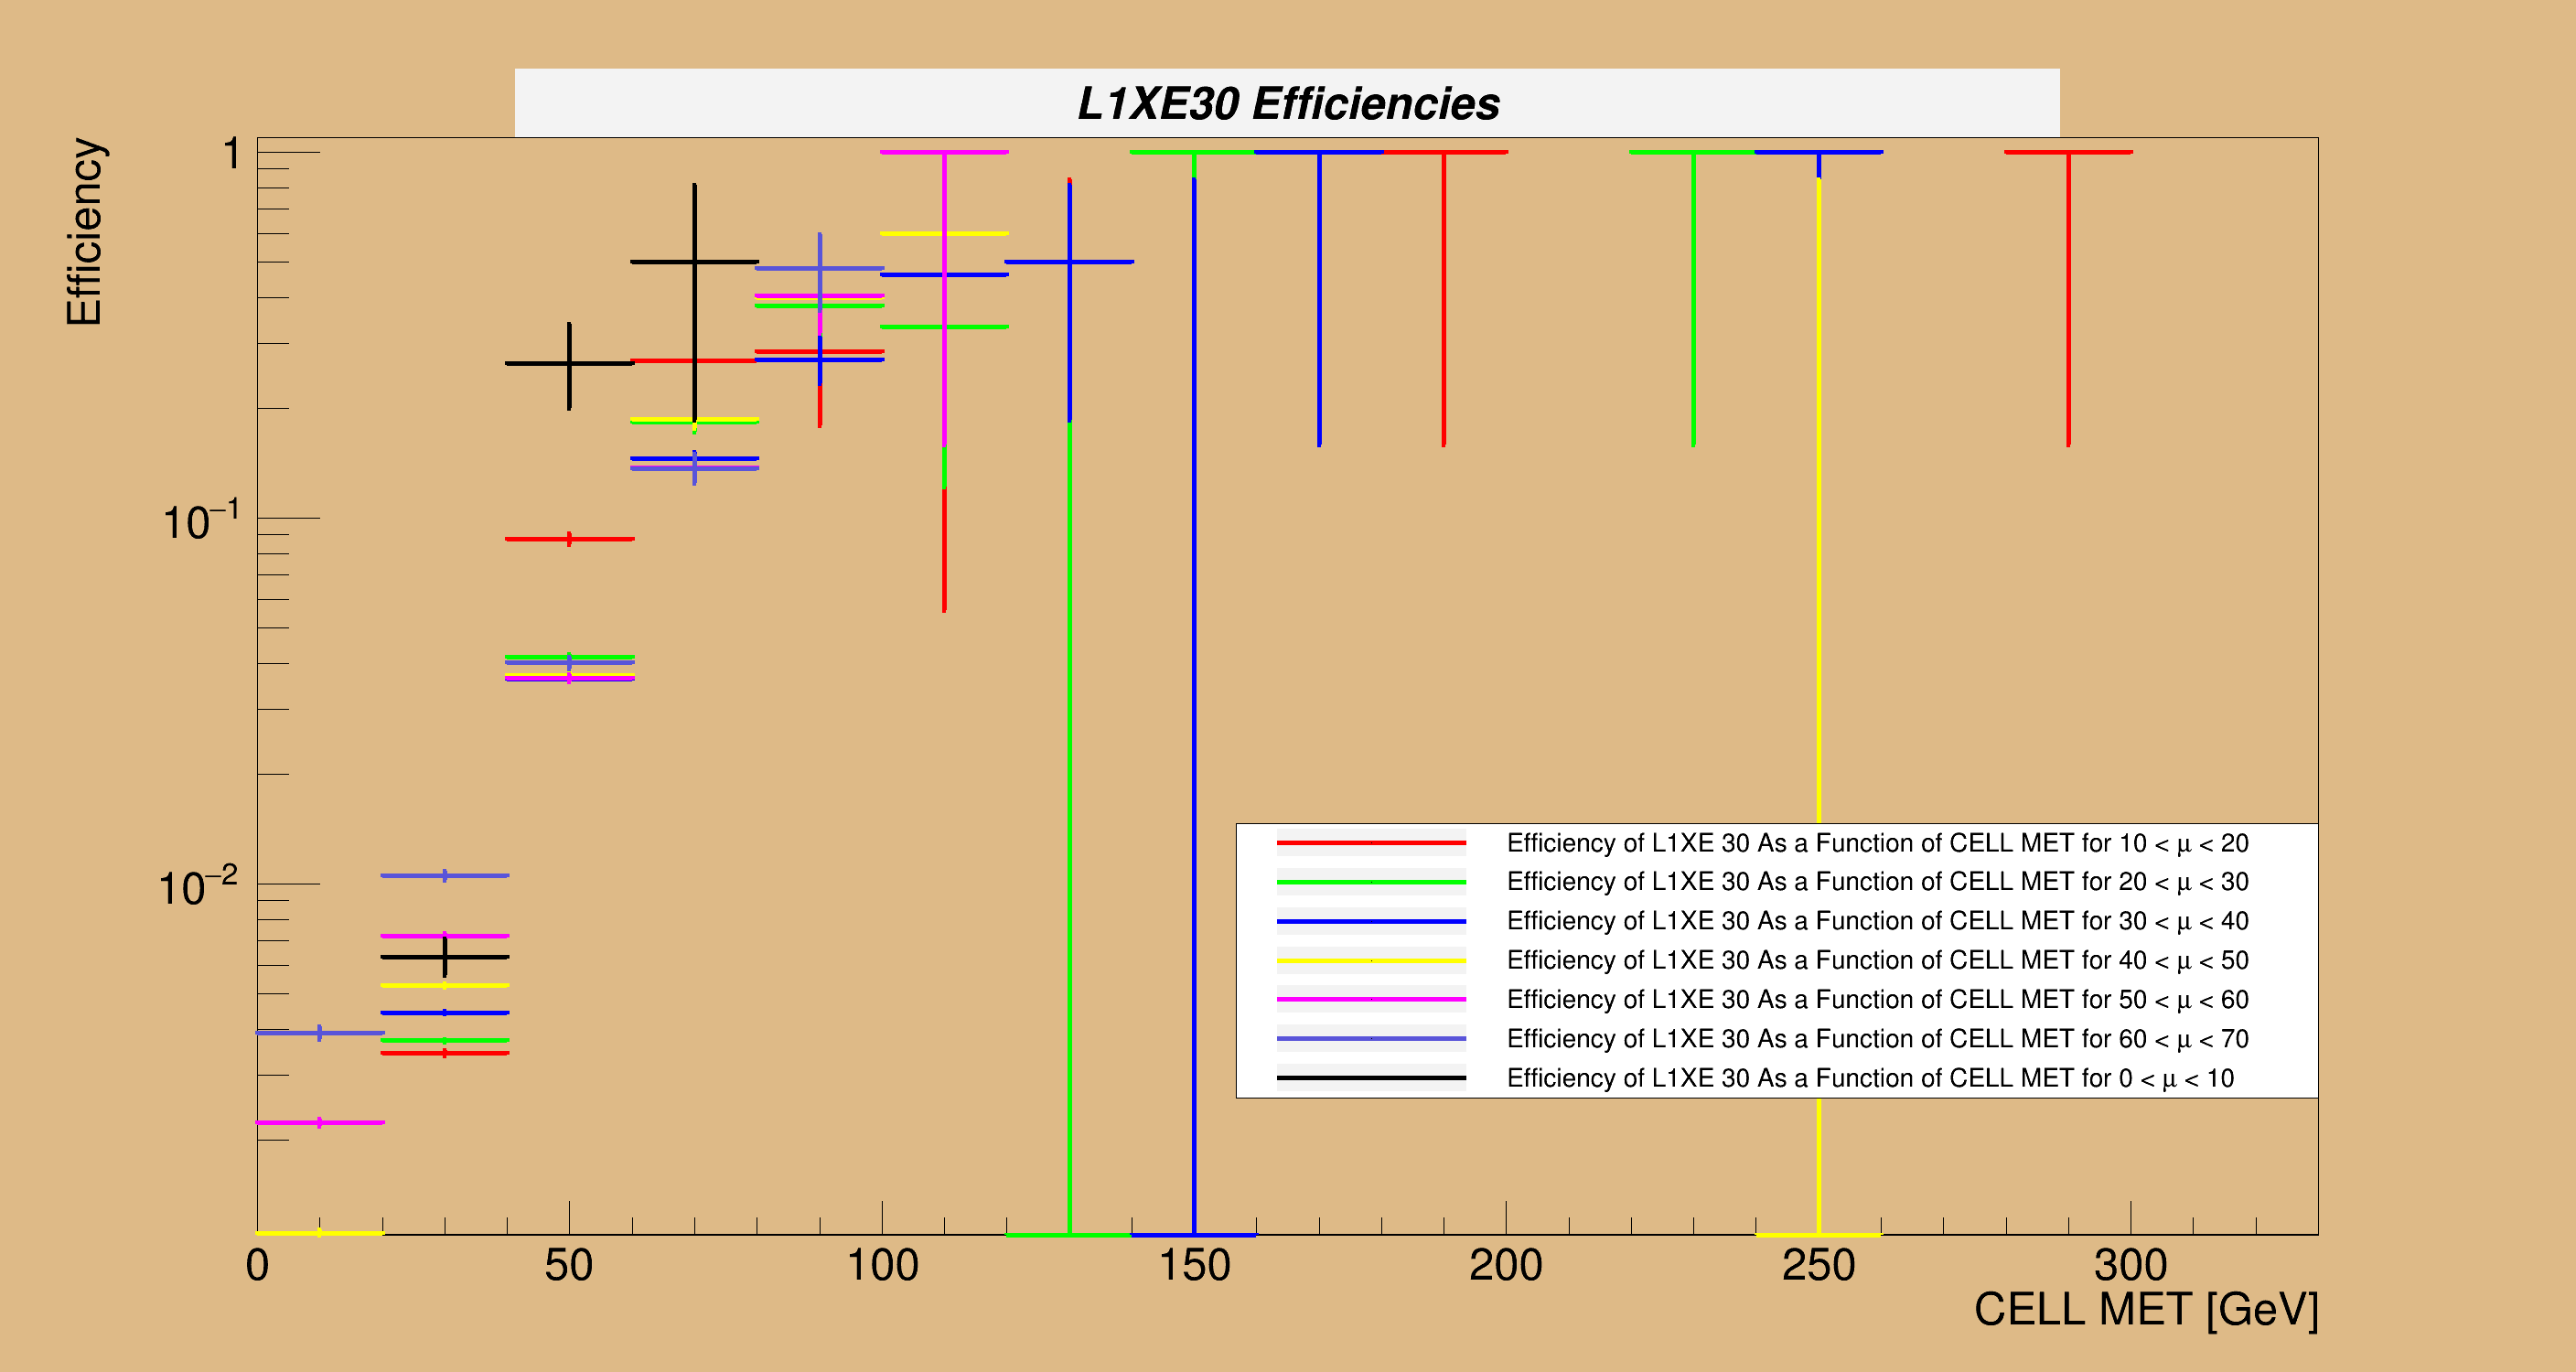
\includegraphics[height=2.65in,width=4.25in]{L1XE30Efficiency_Curves}}
\end{frame}
\begin{frame}
		\framebox{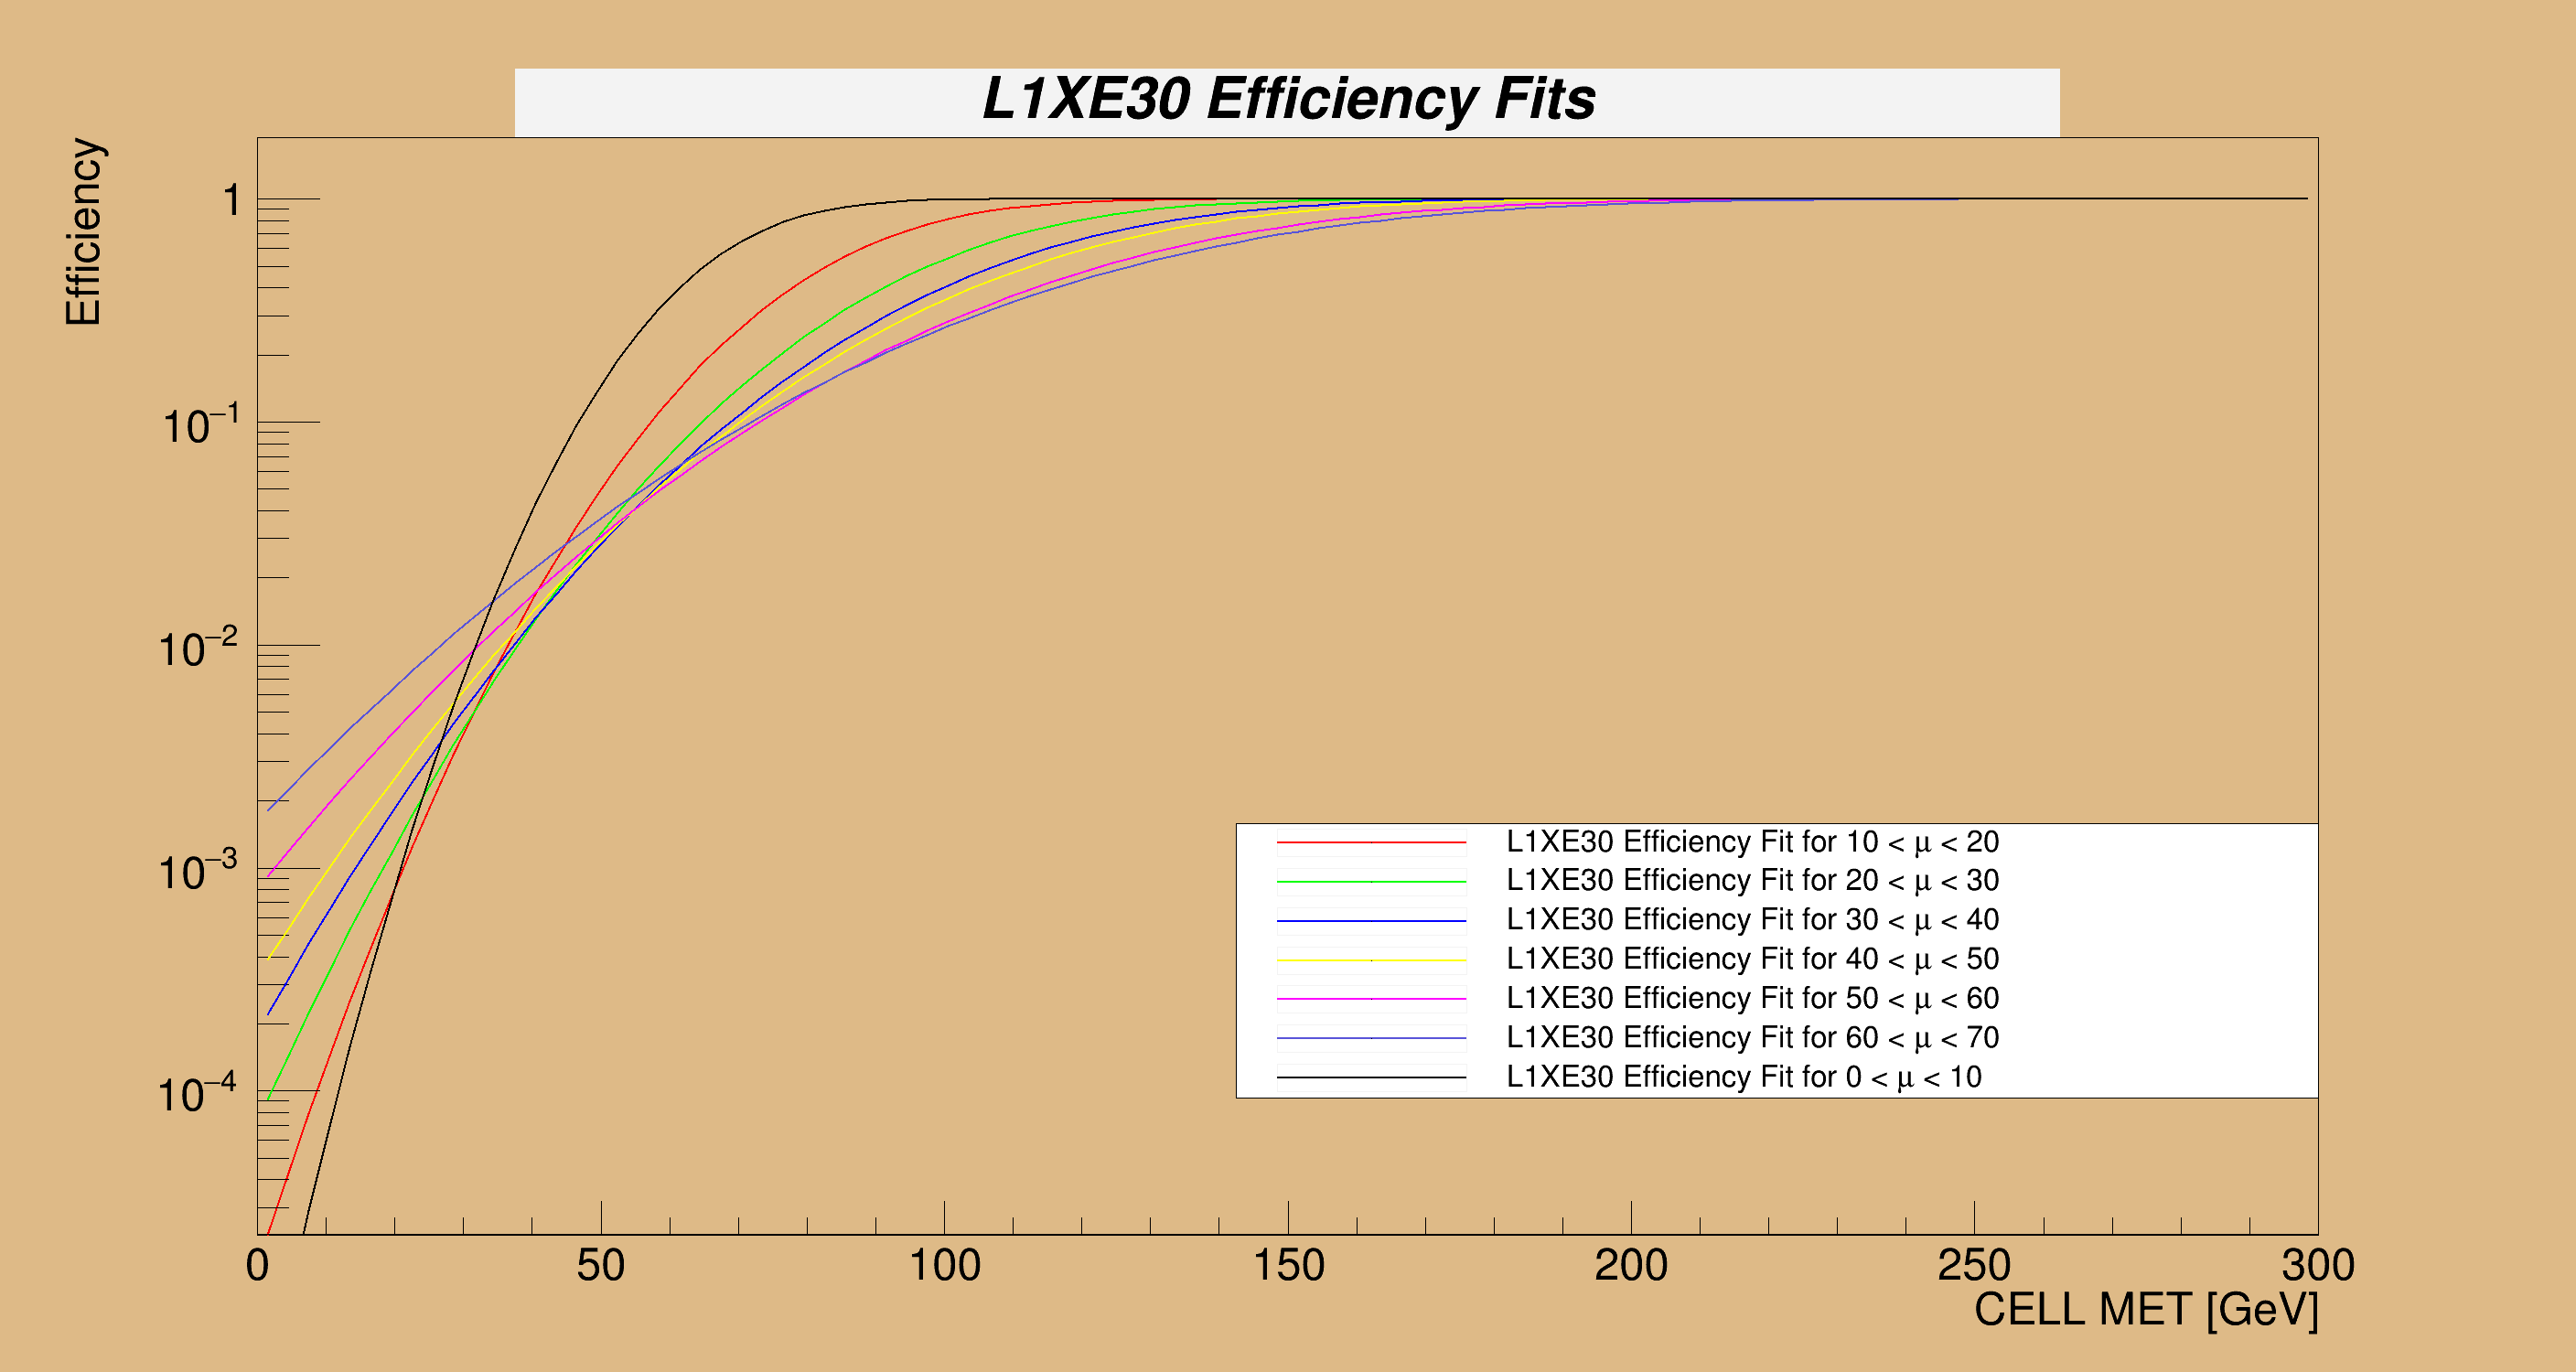
\includegraphics[height=2.65in,width=4.25in]{L1XE30Efficiency_Fits}}
\end{frame}
\begin{frame}
		\framebox{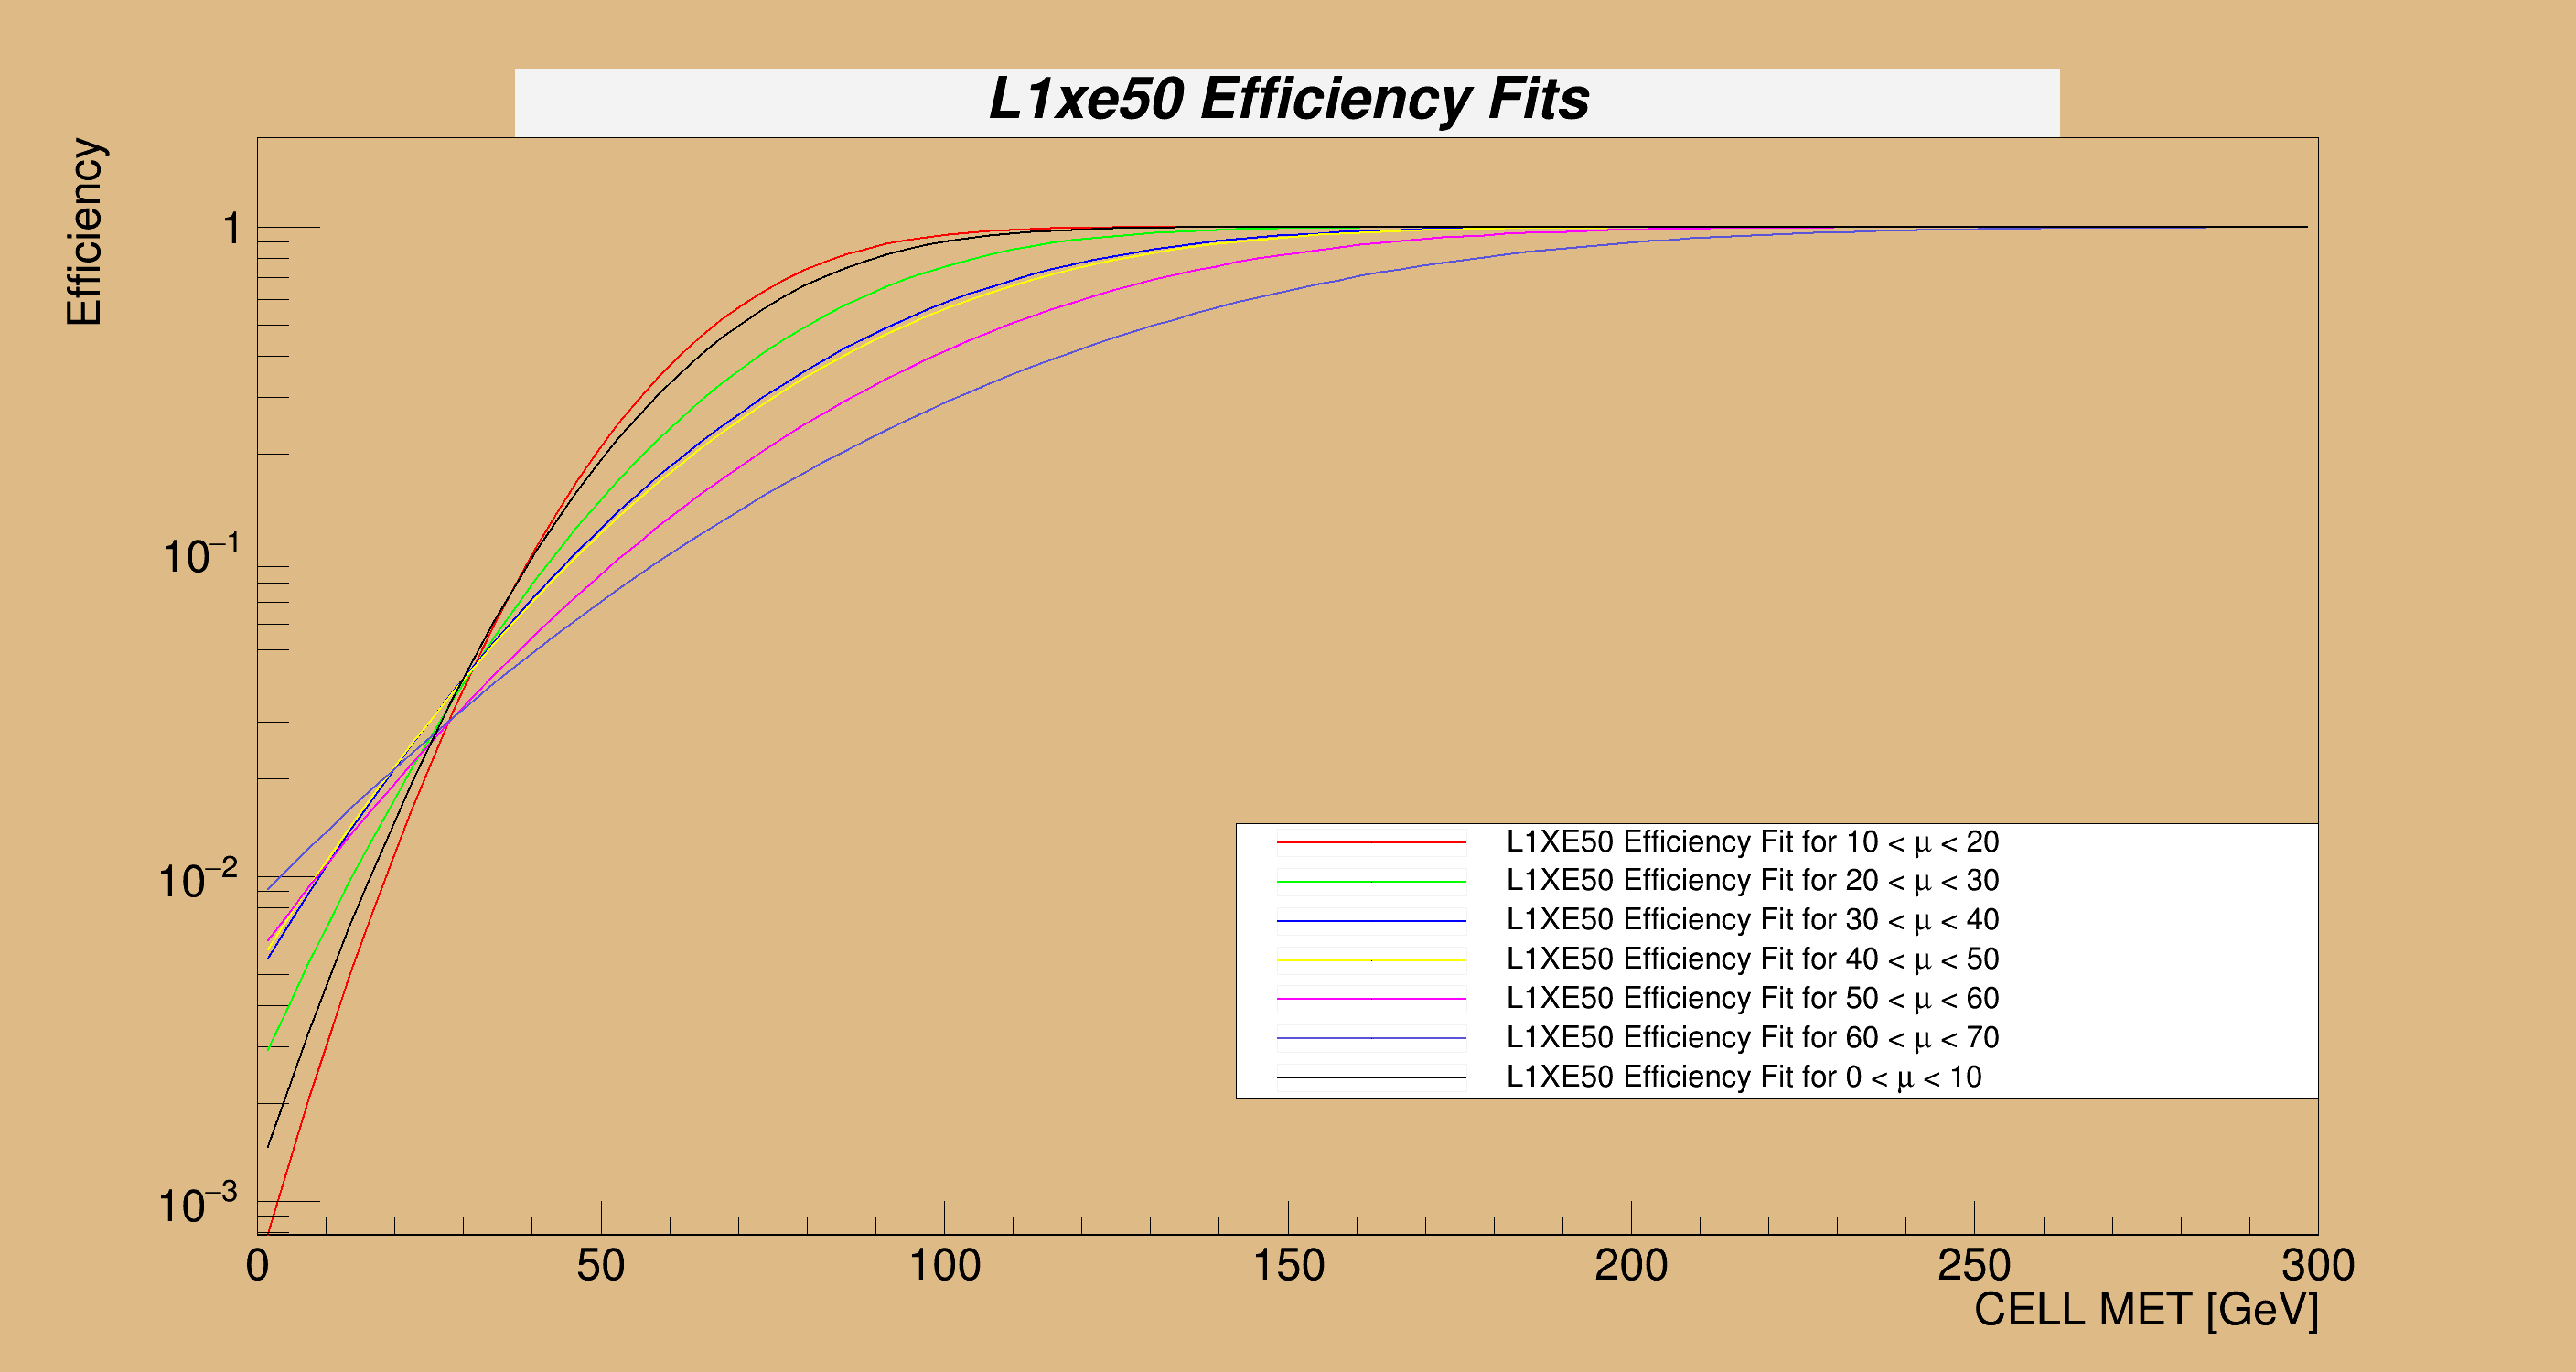
\includegraphics[height=2.65in,width=4.25in]{L1XE50Efficiency_Fits}}
\end{frame}
\begin{frame}
		\framebox{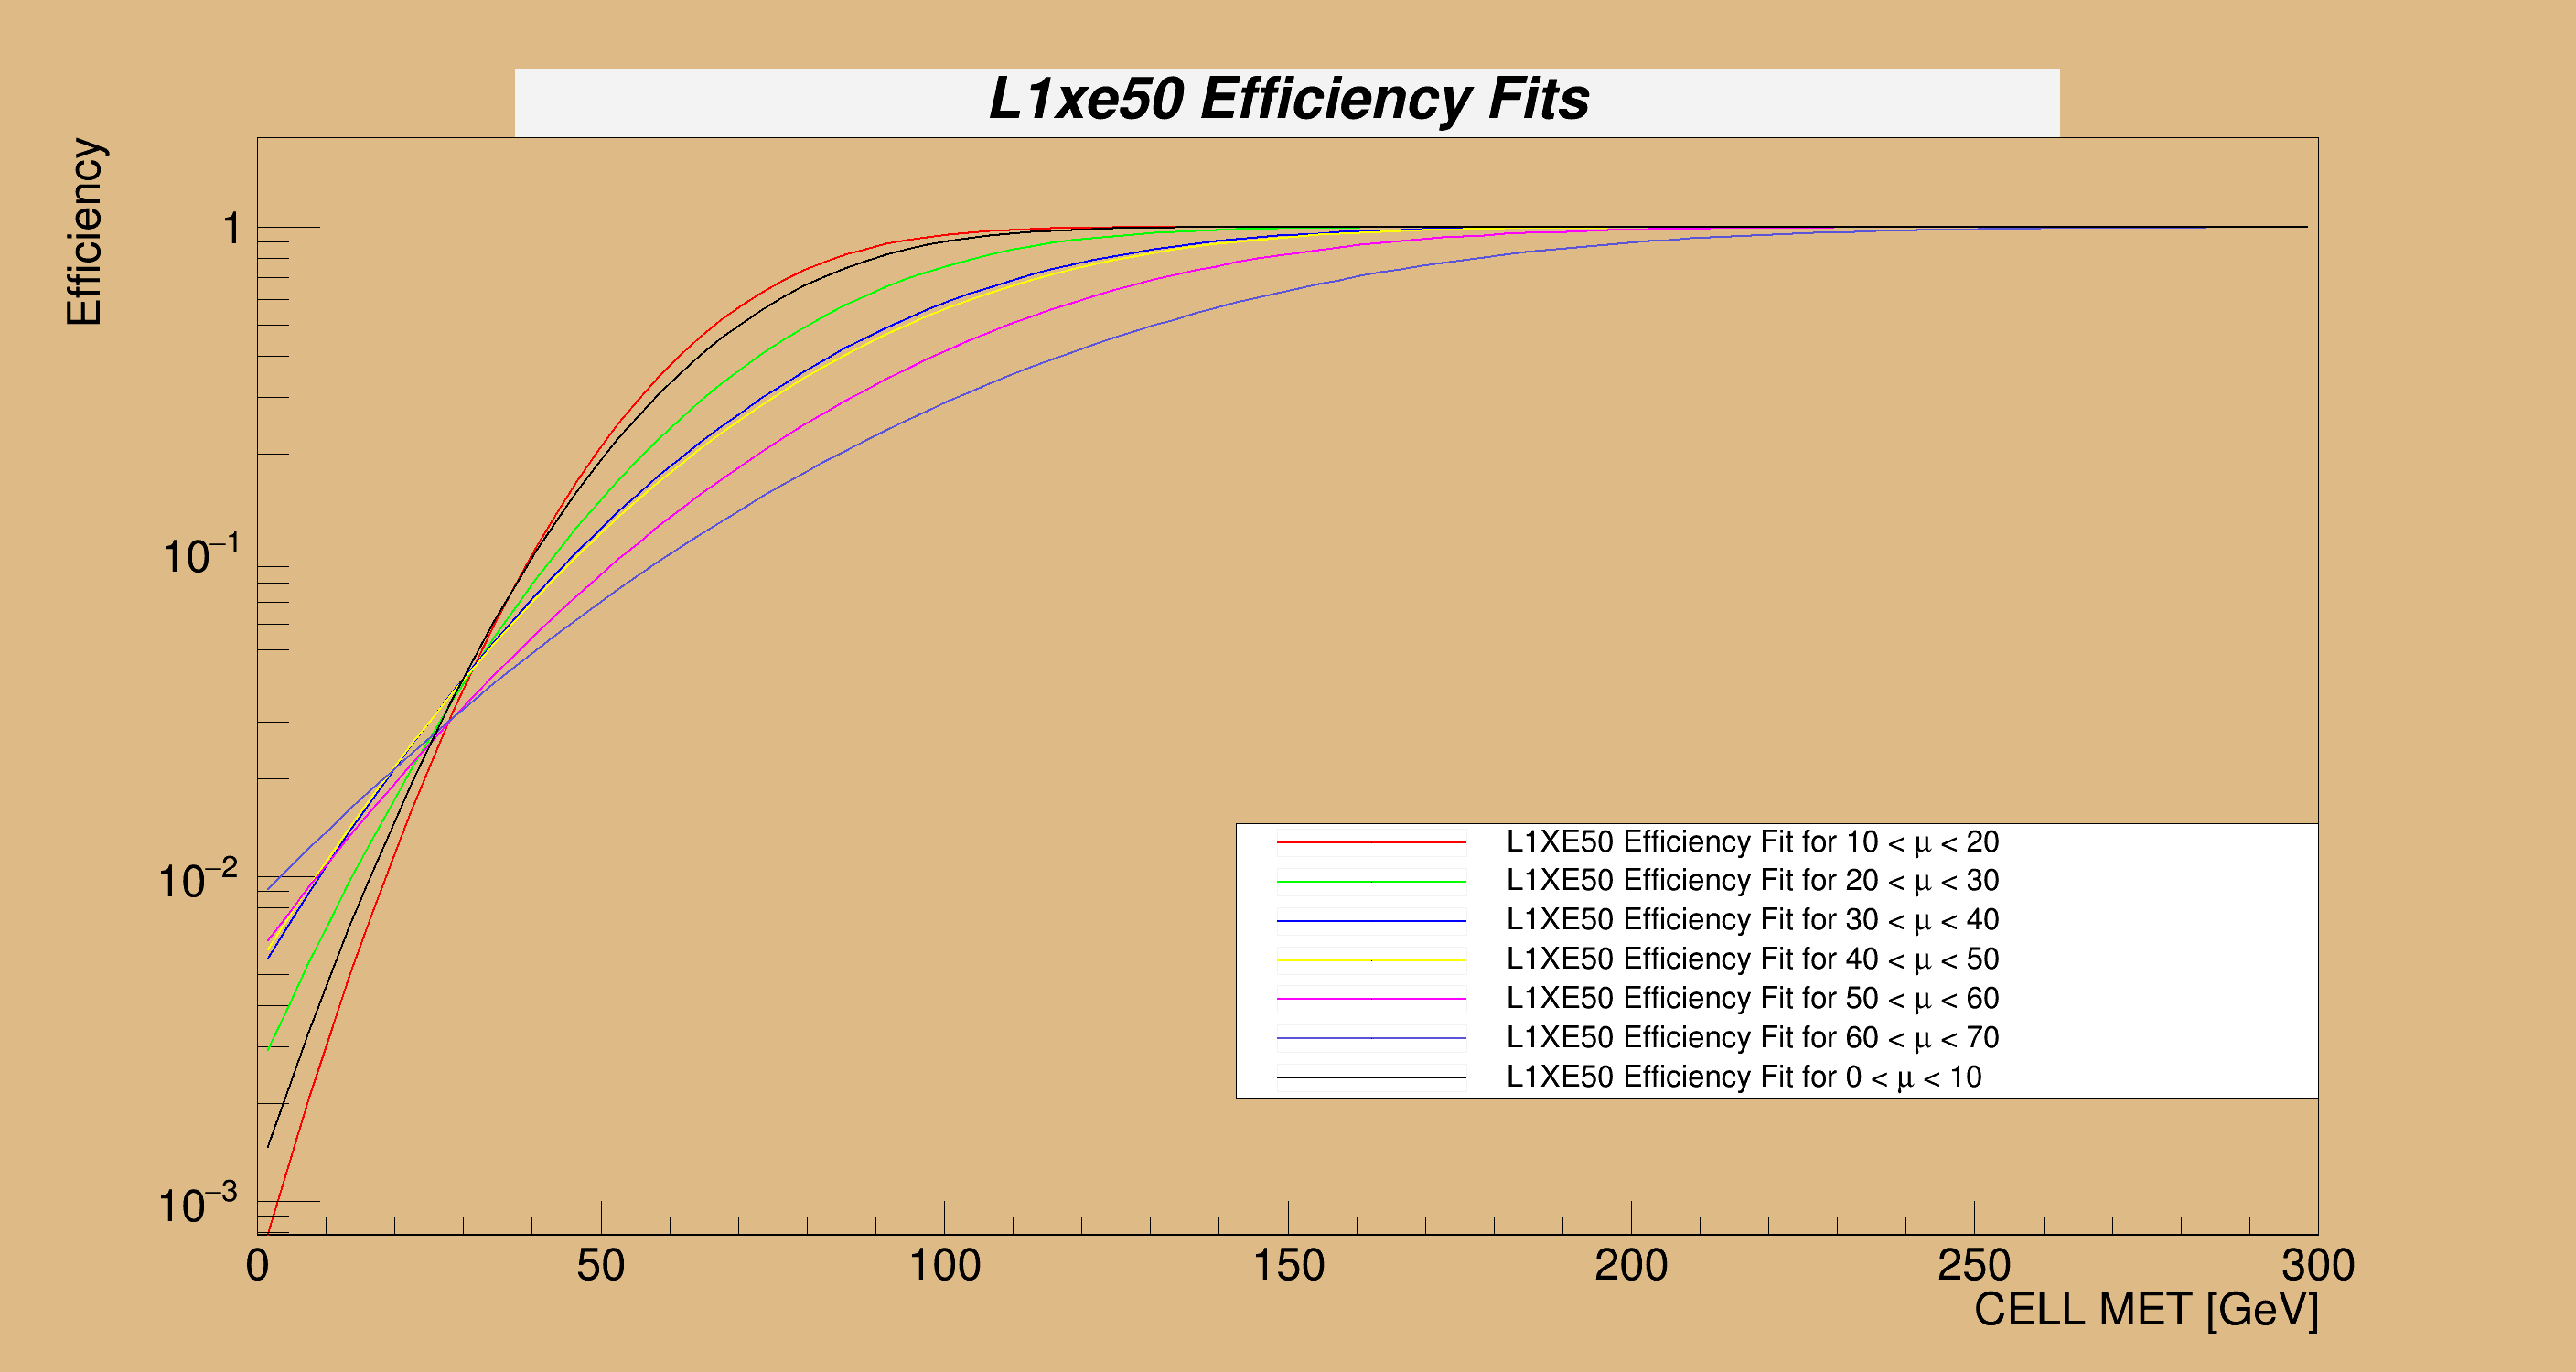
\includegraphics[height=2.65in,width=4.25in]{L1XE50Efficiency_Fits}}
\end{frame}
\section{Performing Correction}
\begin{frame}{Correcting the \texttt{HLTnoalg} Distribution}
		\begin{itemize}
				\item After computing the efficiency curves for the cuts on L1, the curves were used to correct the HLTnoalg distributions that are biased with respect to L1 so that they replicate the unbiased distribution
				\item In order to do this, it was necessary to multiply by the recorded prescale, and divide by the efficiency used to correct the data
				\begin{itemize}
						\item For the \texttt{HLTnoalg\_L1XE30} data, we used the \texttt{L1XE30} efficiency curve to correct the distribution
						\item For the \texttt{HLTnoalg\_L1XE50} data we used the \texttt{L1XE30} efficiency of the zerobias data, as well as the L1XE50 efficiency of \texttt{HLTnoalg\_L1XE30} data to correct the distribution
				\end{itemize}
		\end{itemize}
\end{frame}
\section{Error Propagation}
\begin{frame}{Error Propagation}
		\begin{itemize}
				\item The error in each efficiency value is determined by propagating the errors on the parameters of the respective fit function.
				\item The reconstructed MET distribution includes both the error determined above, and the statistical error. 
				\item Since prescales vary for each bin, must keep track of errors event by event, rather than using ROOT’s built-in errors. 
				\item Kept track of the errors on the \texttt{L1XE30} corrected curves, as well as the \texttt{L1XE50} corrected curves, for each of the mu bins
				\item There is no error included to reflect the fact that the error function may not be a perfect model. Therefore, in final distribution, zerobias data is kept to as high an MET as possible and similarly for keeping \texttt{HLTnoalg\_L1XE30} versus \texttt{L1XE50
	} \end{itemize}
\end{frame}
\begin{frame}
		\framebox{\includegraphics[height=2.65in,width=4.25in]{hlt_noalg_l1xe30_plots/hlt_noalg_L1XE30_dist_mubin_3}}
\end{frame}
\begin{frame}
		\framebox{\includegraphics[height=2.65in,width=4.25in]{hlt_noalg_l1xe50_plots/hlt_noalg_L1XE50_dist_mubin_3}}
\end{frame}
\section{Relative Normalization}
\begin{frame}{Relative Normalization}
		\begin{itemize}
				\item Because the error bars are larger at low values of MET, it is not sufficient to normalize the entire curve to one. Instead, it was necessary to perform a relative overall normalization between the original zerobias distribution and the corrected curves in order to be able to compare the shapes more easily.
				\item The relative normalization factor was computed by taking a weighted average of ratios computed in the region where the slopes look most parallel.
		\end{itemize}
\end{frame}
\section{Reconstructed Distributions}
\begin{frame}
		\framebox{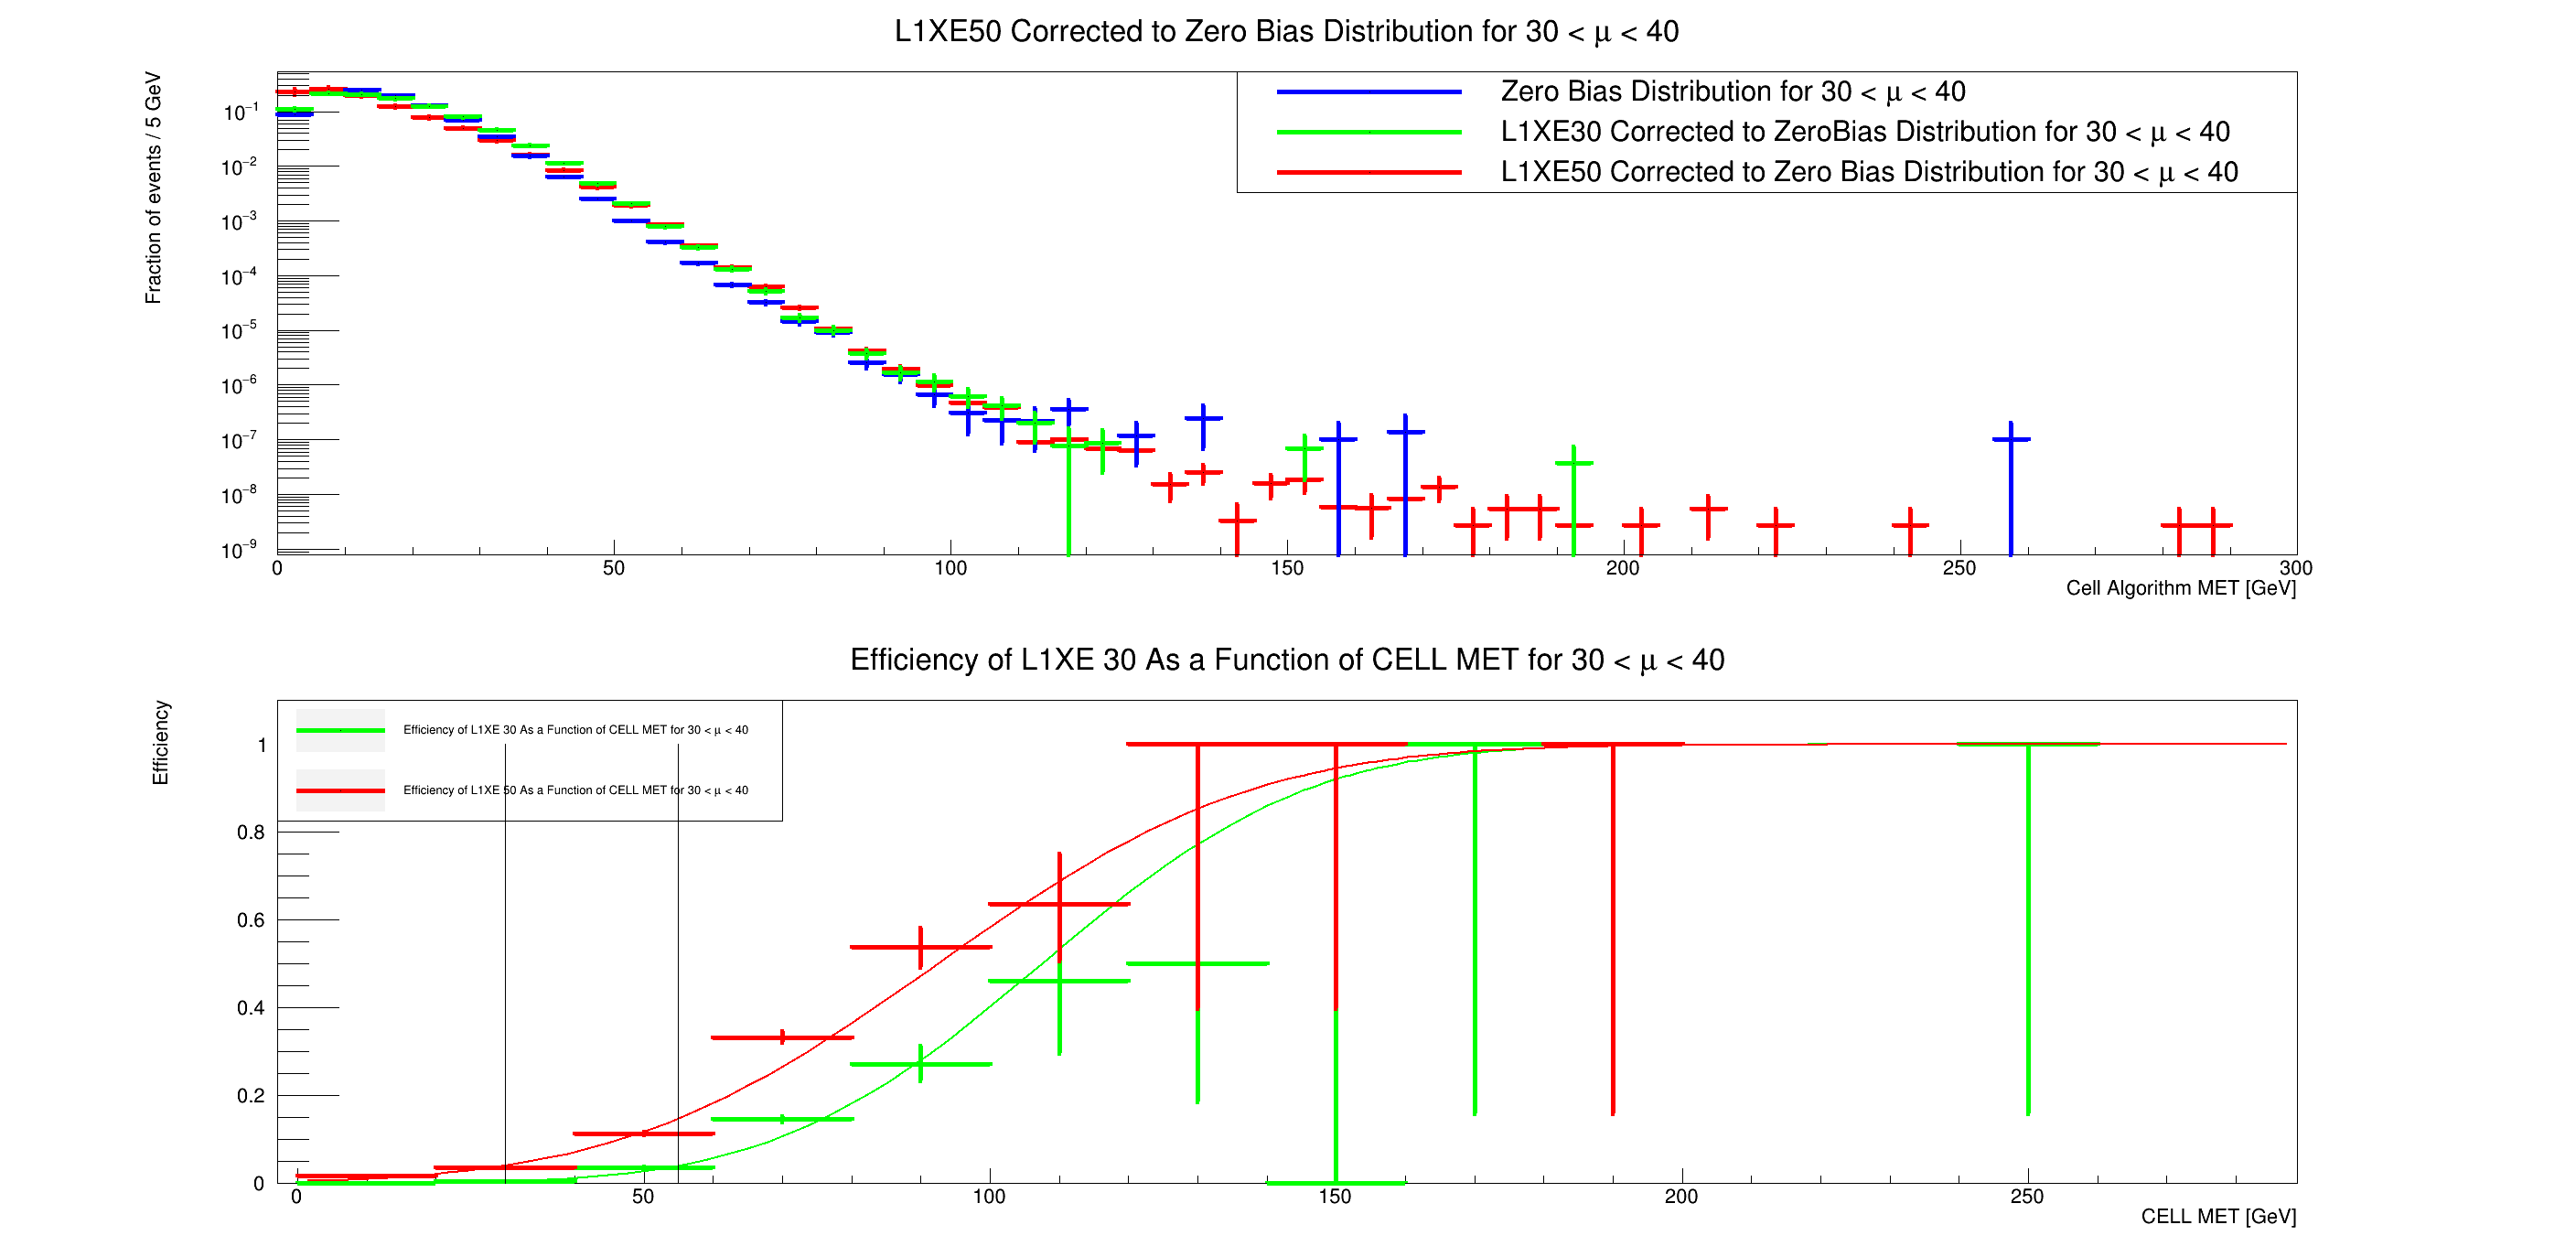
\includegraphics[height=2.65in,width=4.25in]{zerobias_distributions_corrected/zb_met_distributions_mubin_3}}
\end{frame}

\begin{frame}
		\framebox{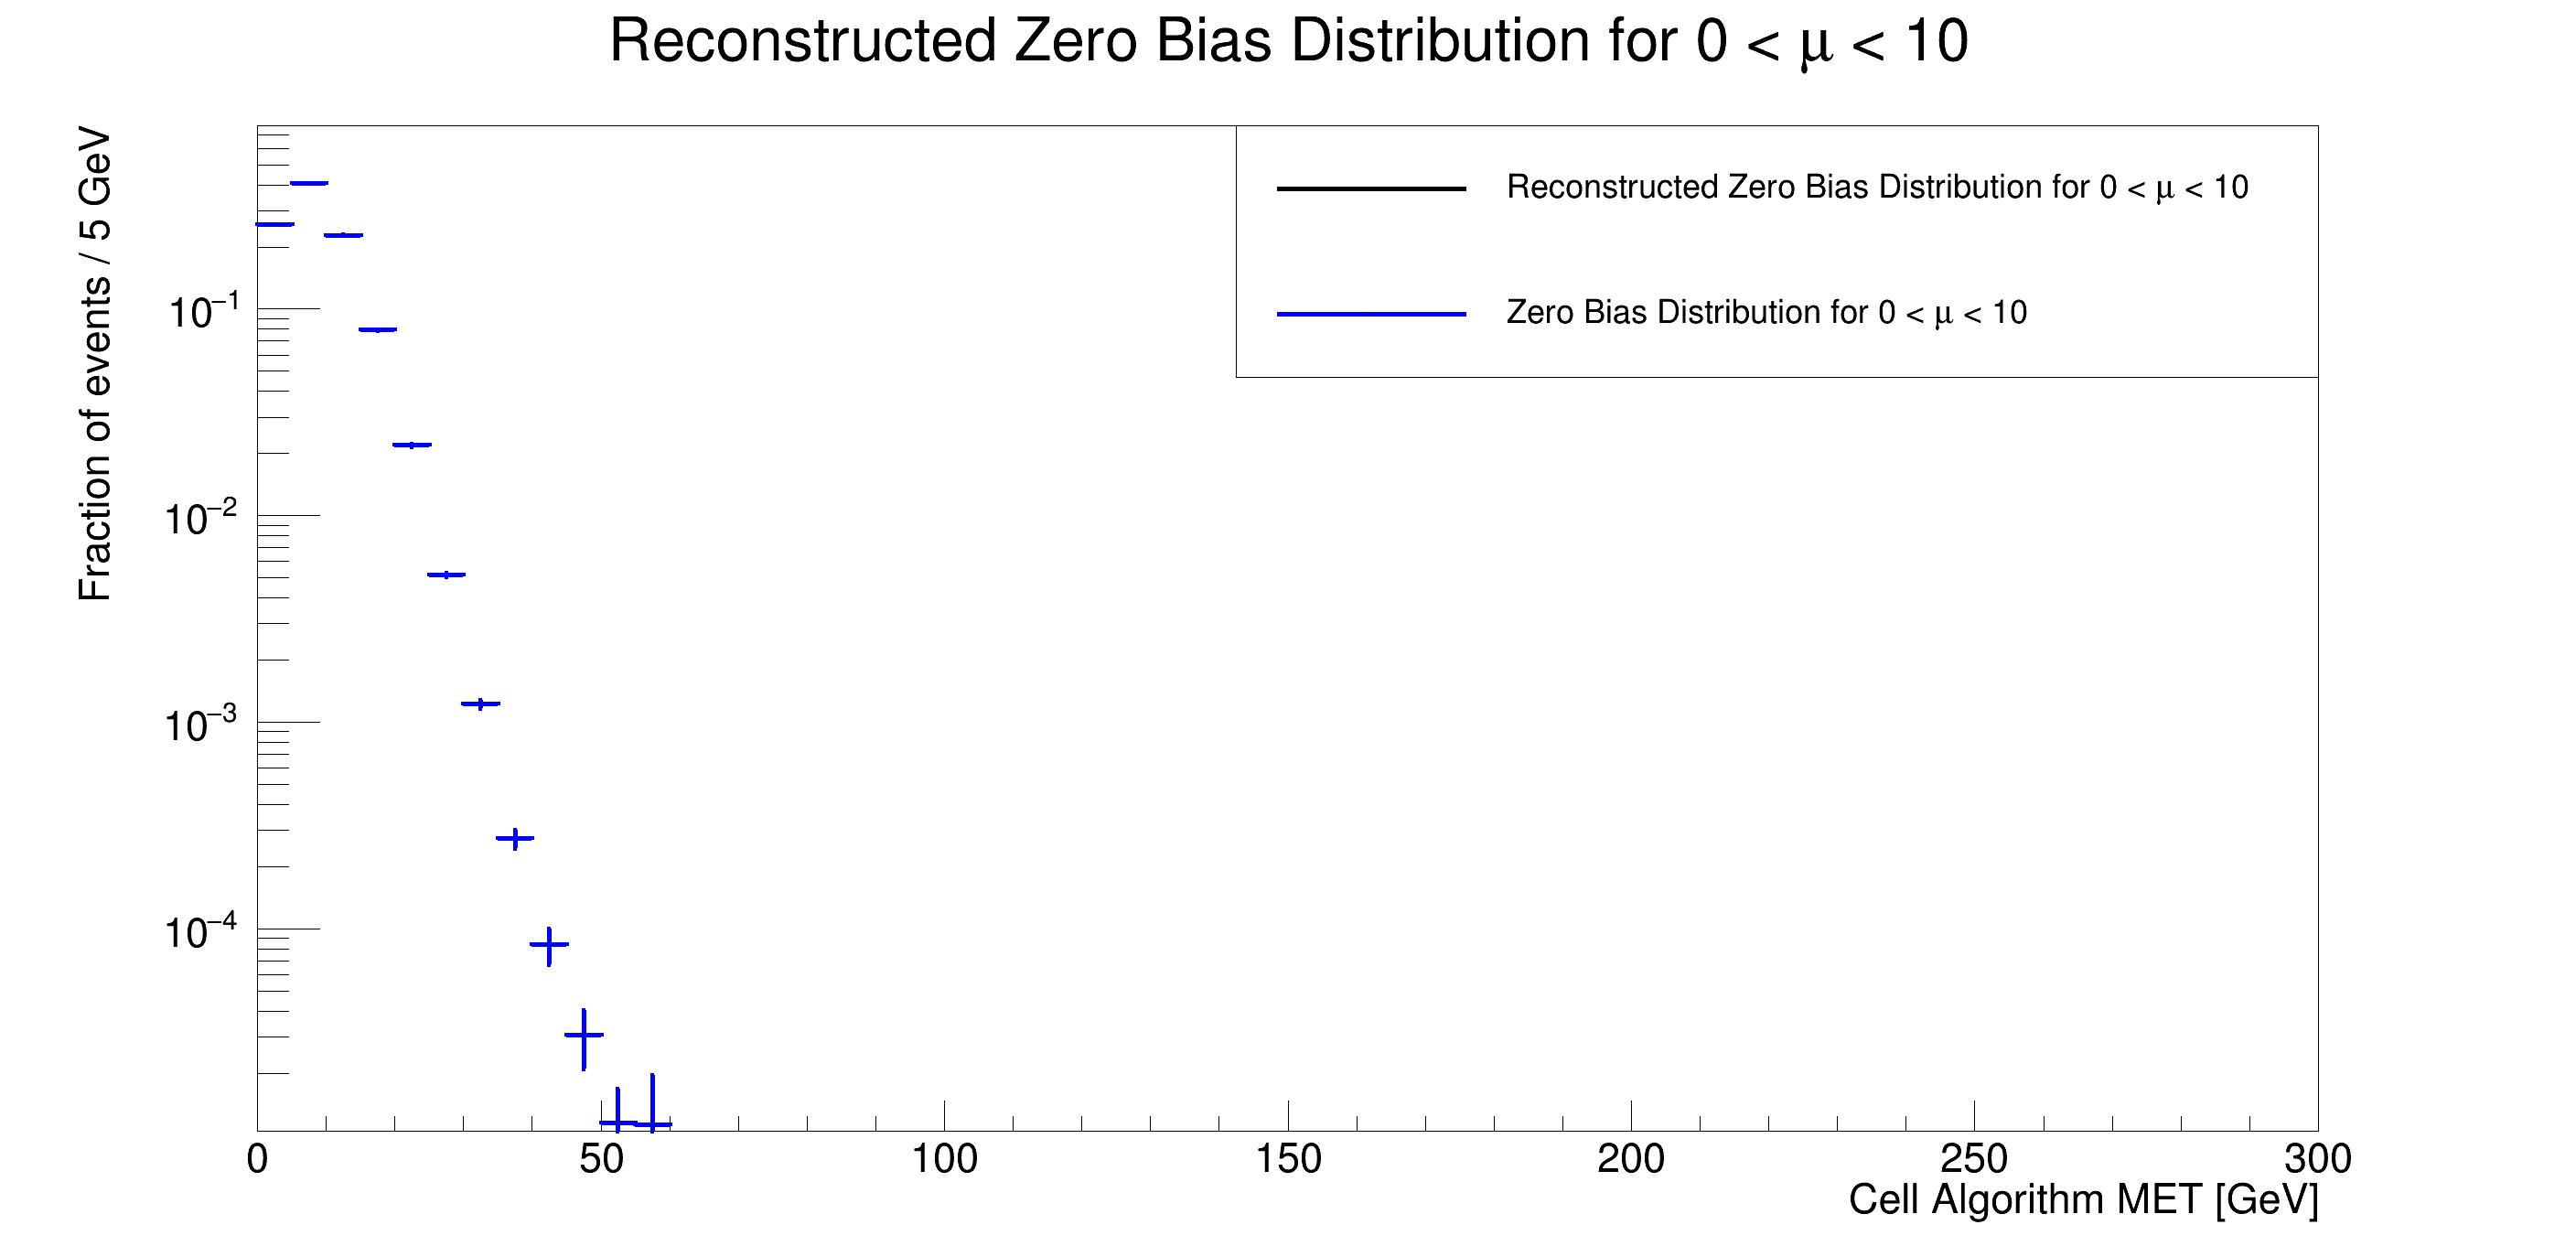
\includegraphics[height=2.65in,width=4.25in]{reconstructed_distributions/reconstructed_distribution_mubin_0}}
\end{frame}
\begin{frame}
		\framebox{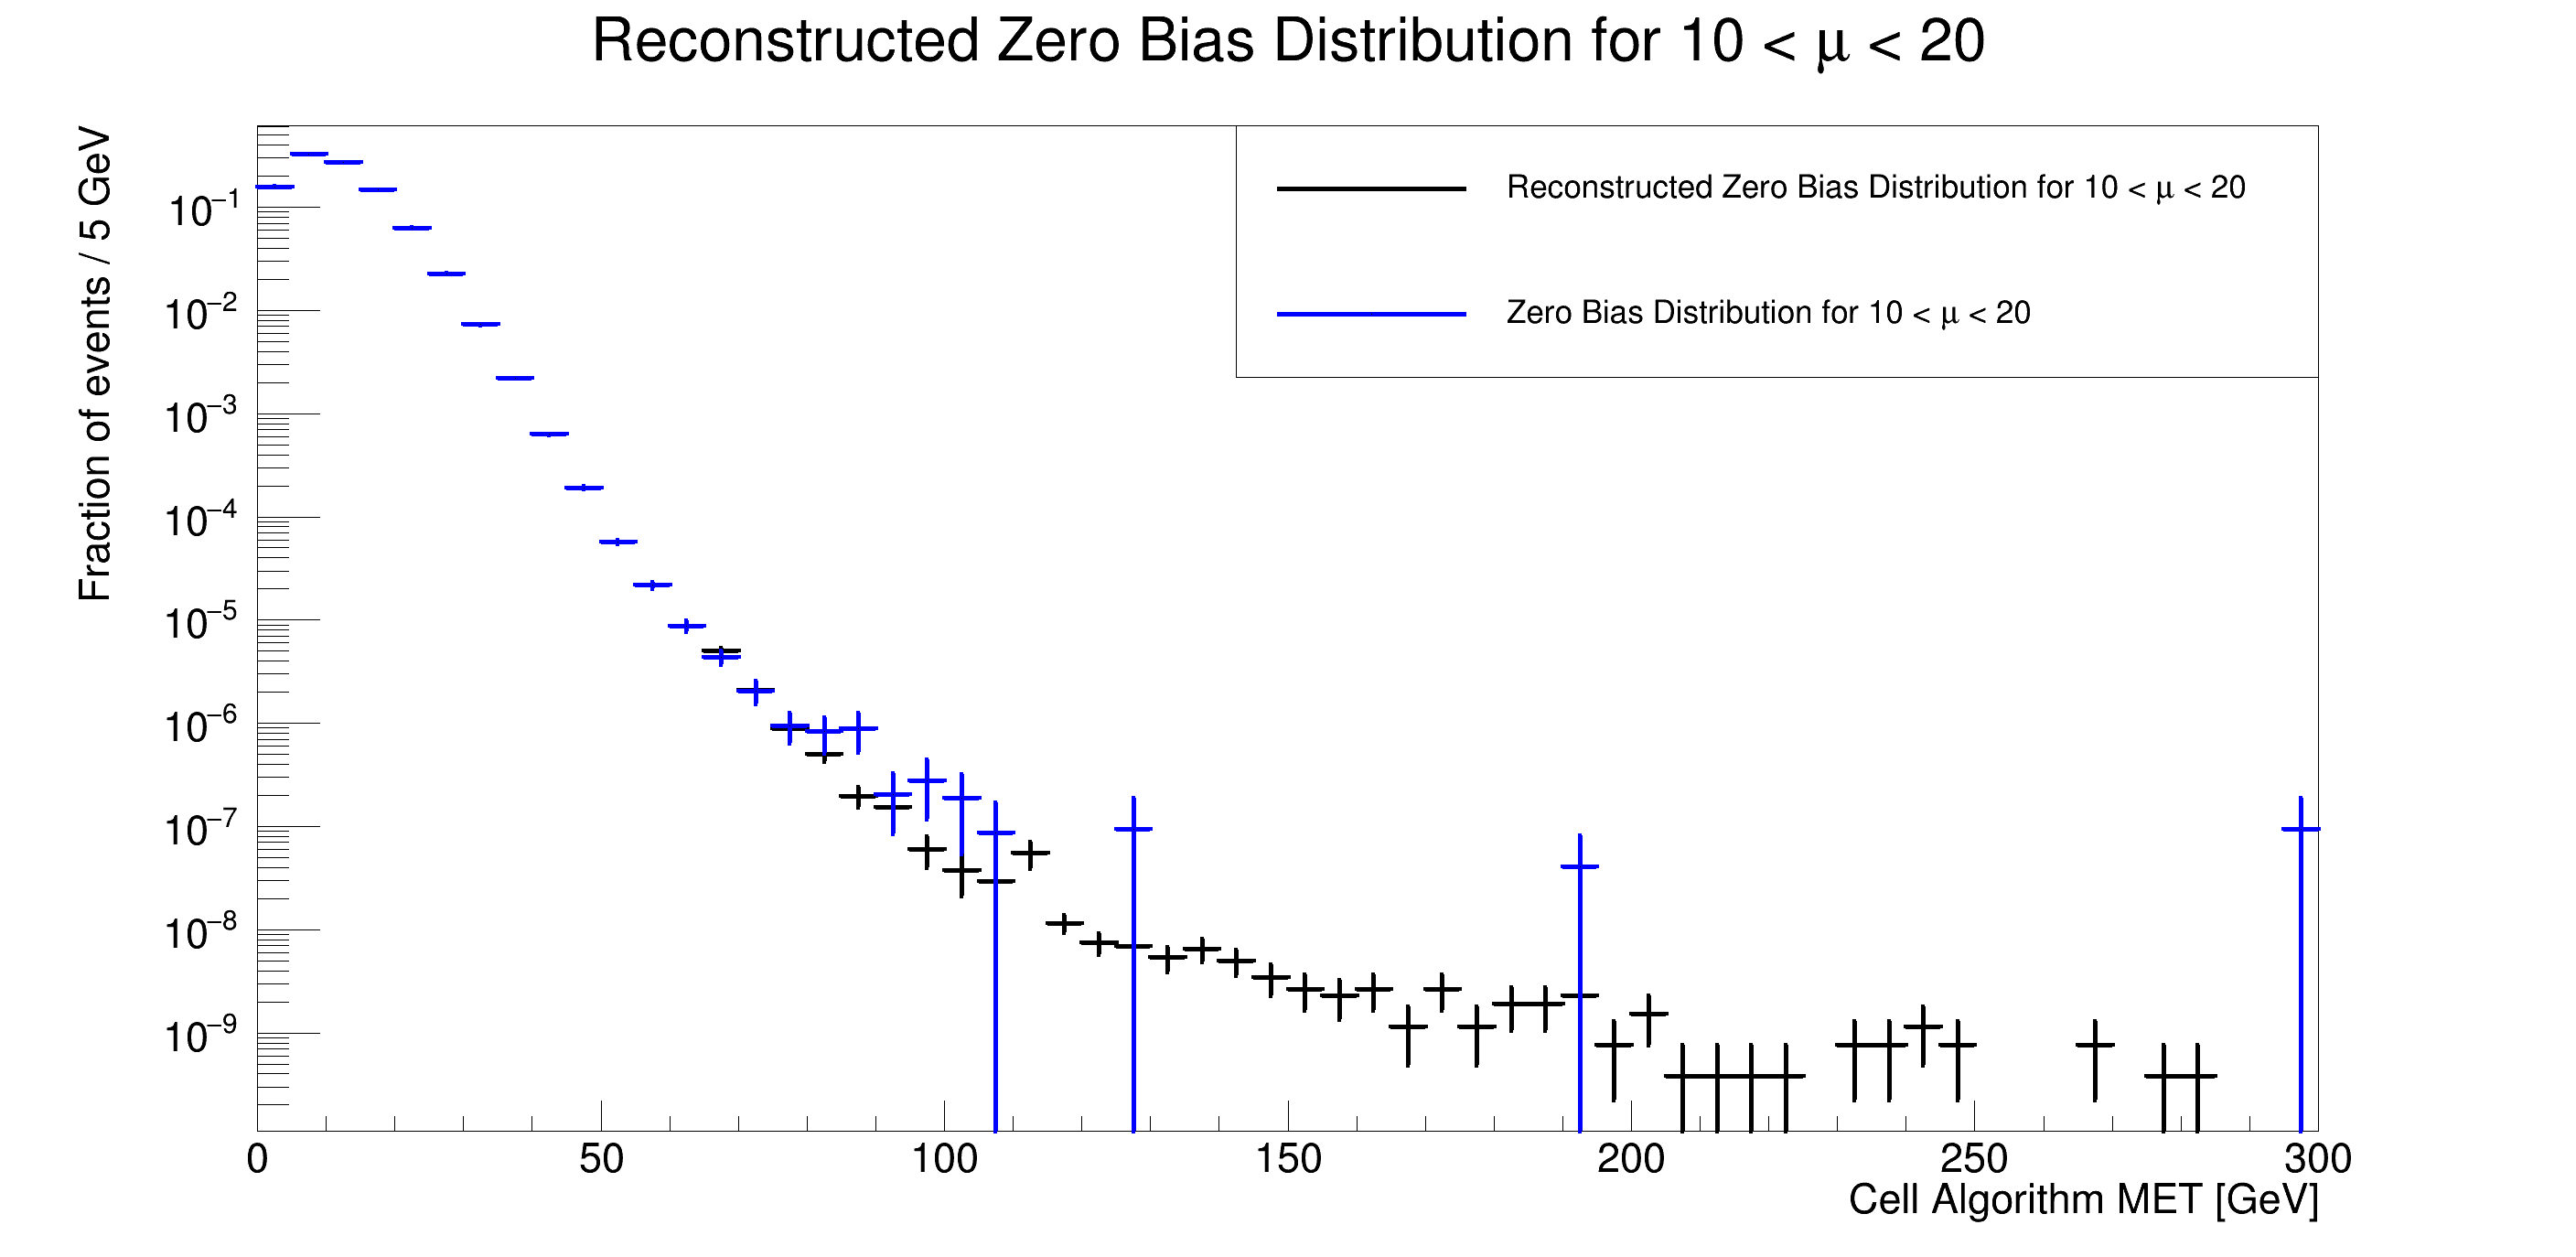
\includegraphics[height=2.65in,width=4.25in]{reconstructed_distributions/reconstructed_distribution_mubin_1}}
\end{frame}
\begin{frame}
		\framebox{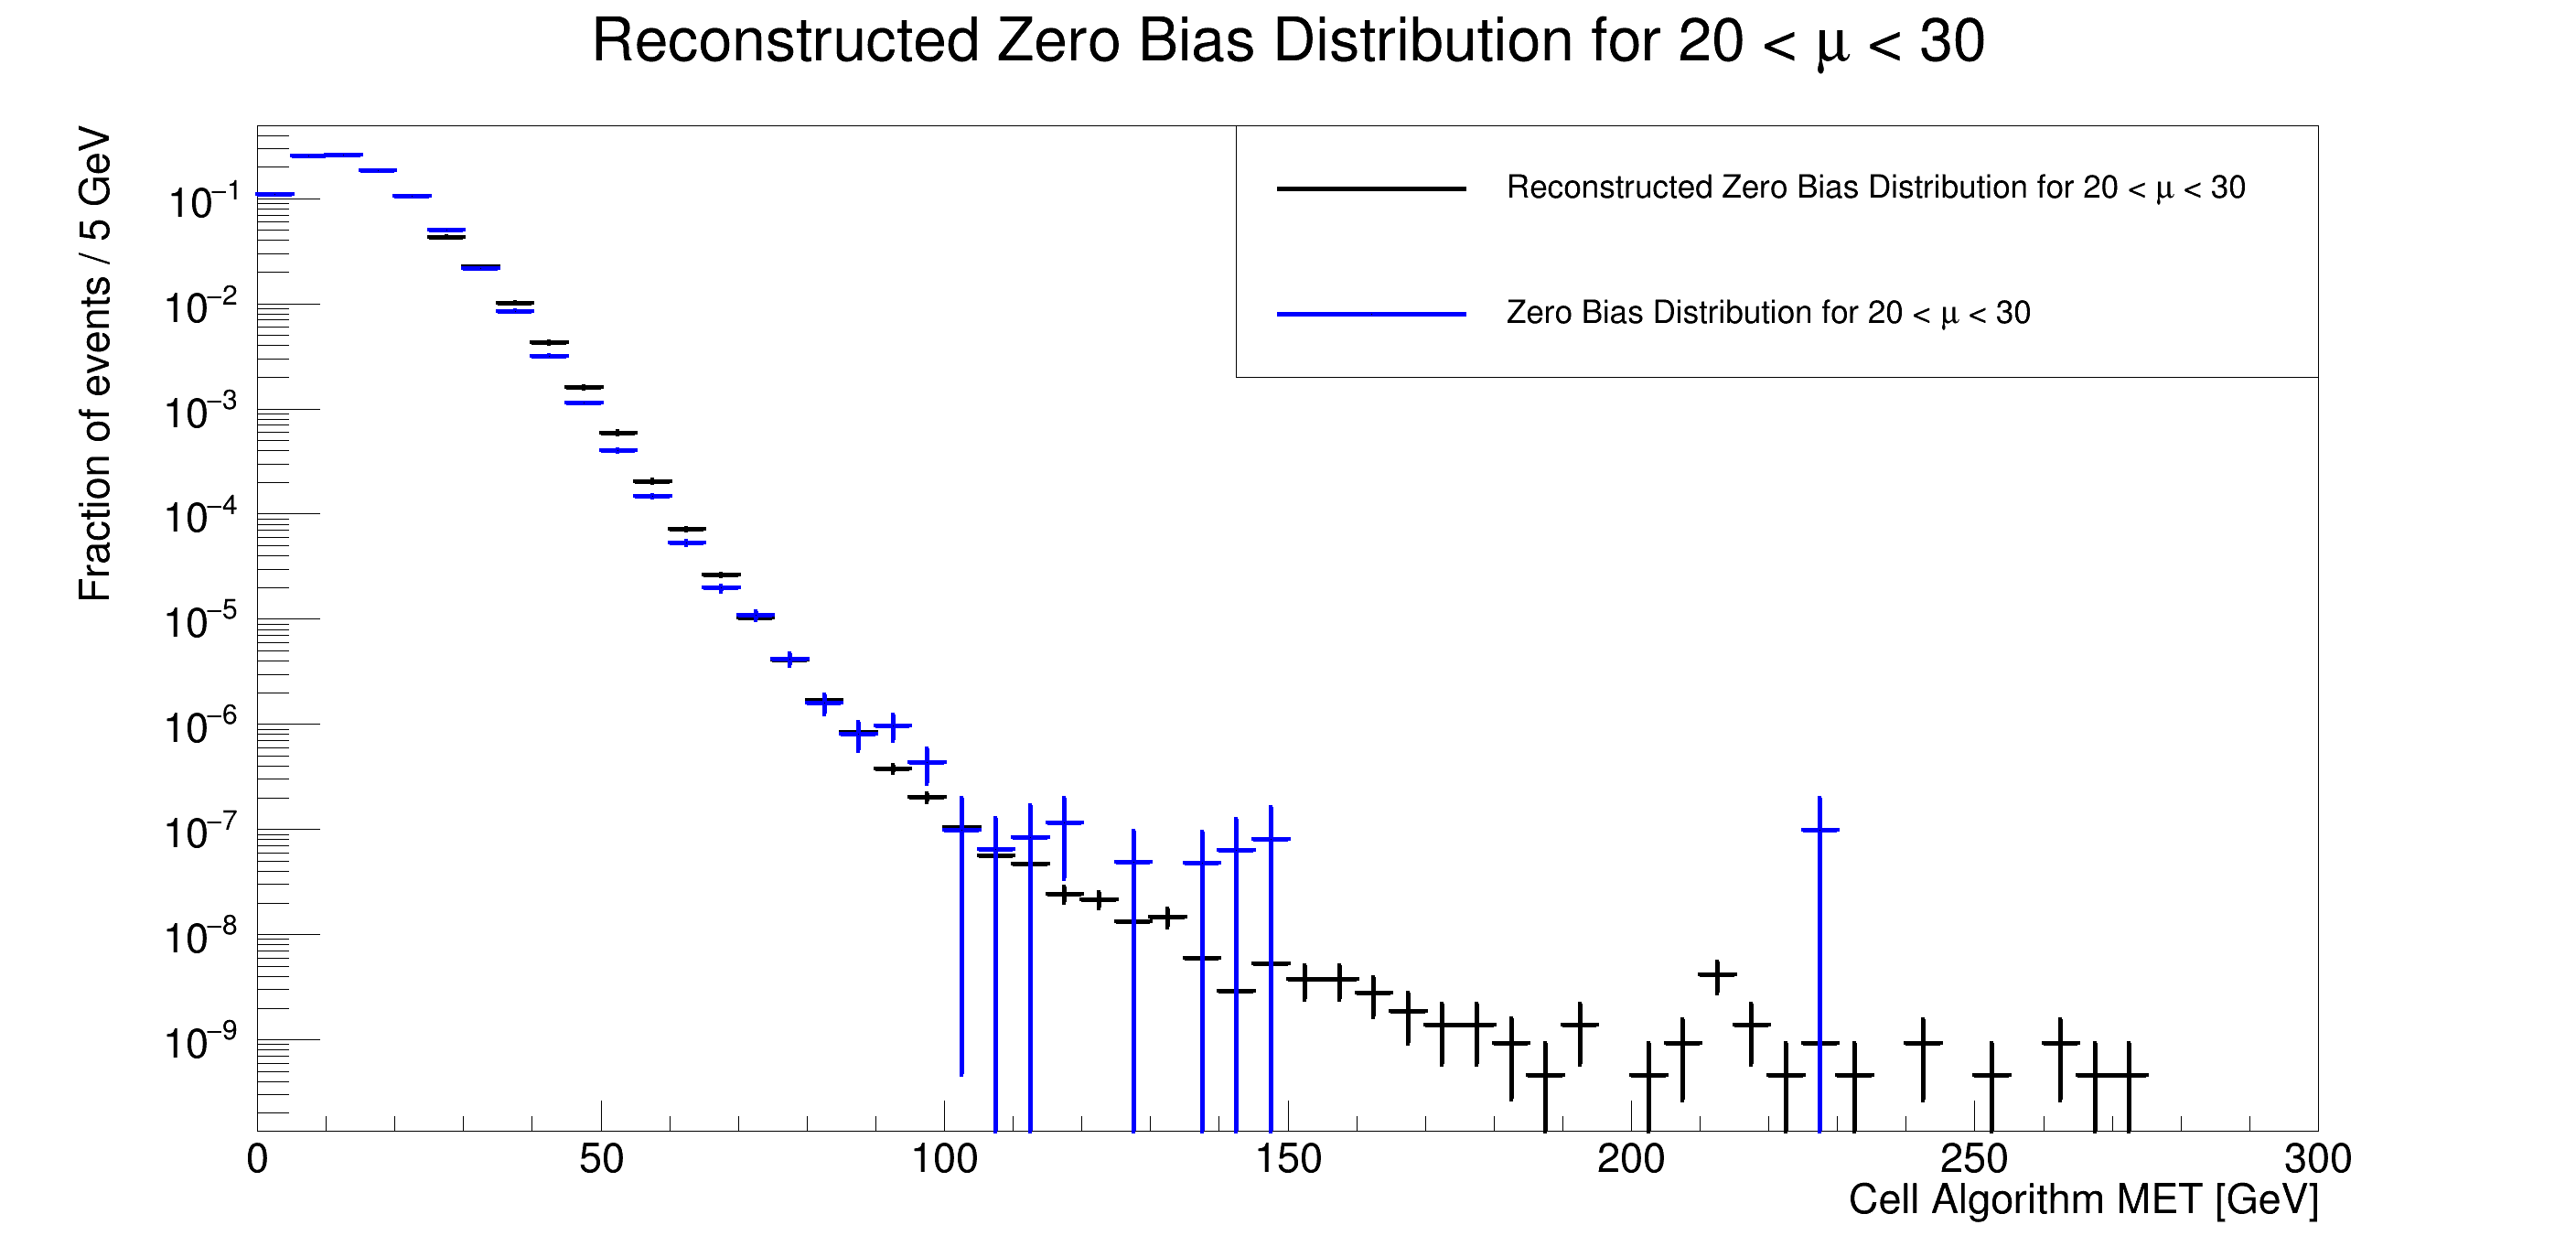
\includegraphics[height=2.65in,width=4.25in]{reconstructed_distributions/reconstructed_distribution_mubin_2}}
\end{frame}
\begin{frame}
		\framebox{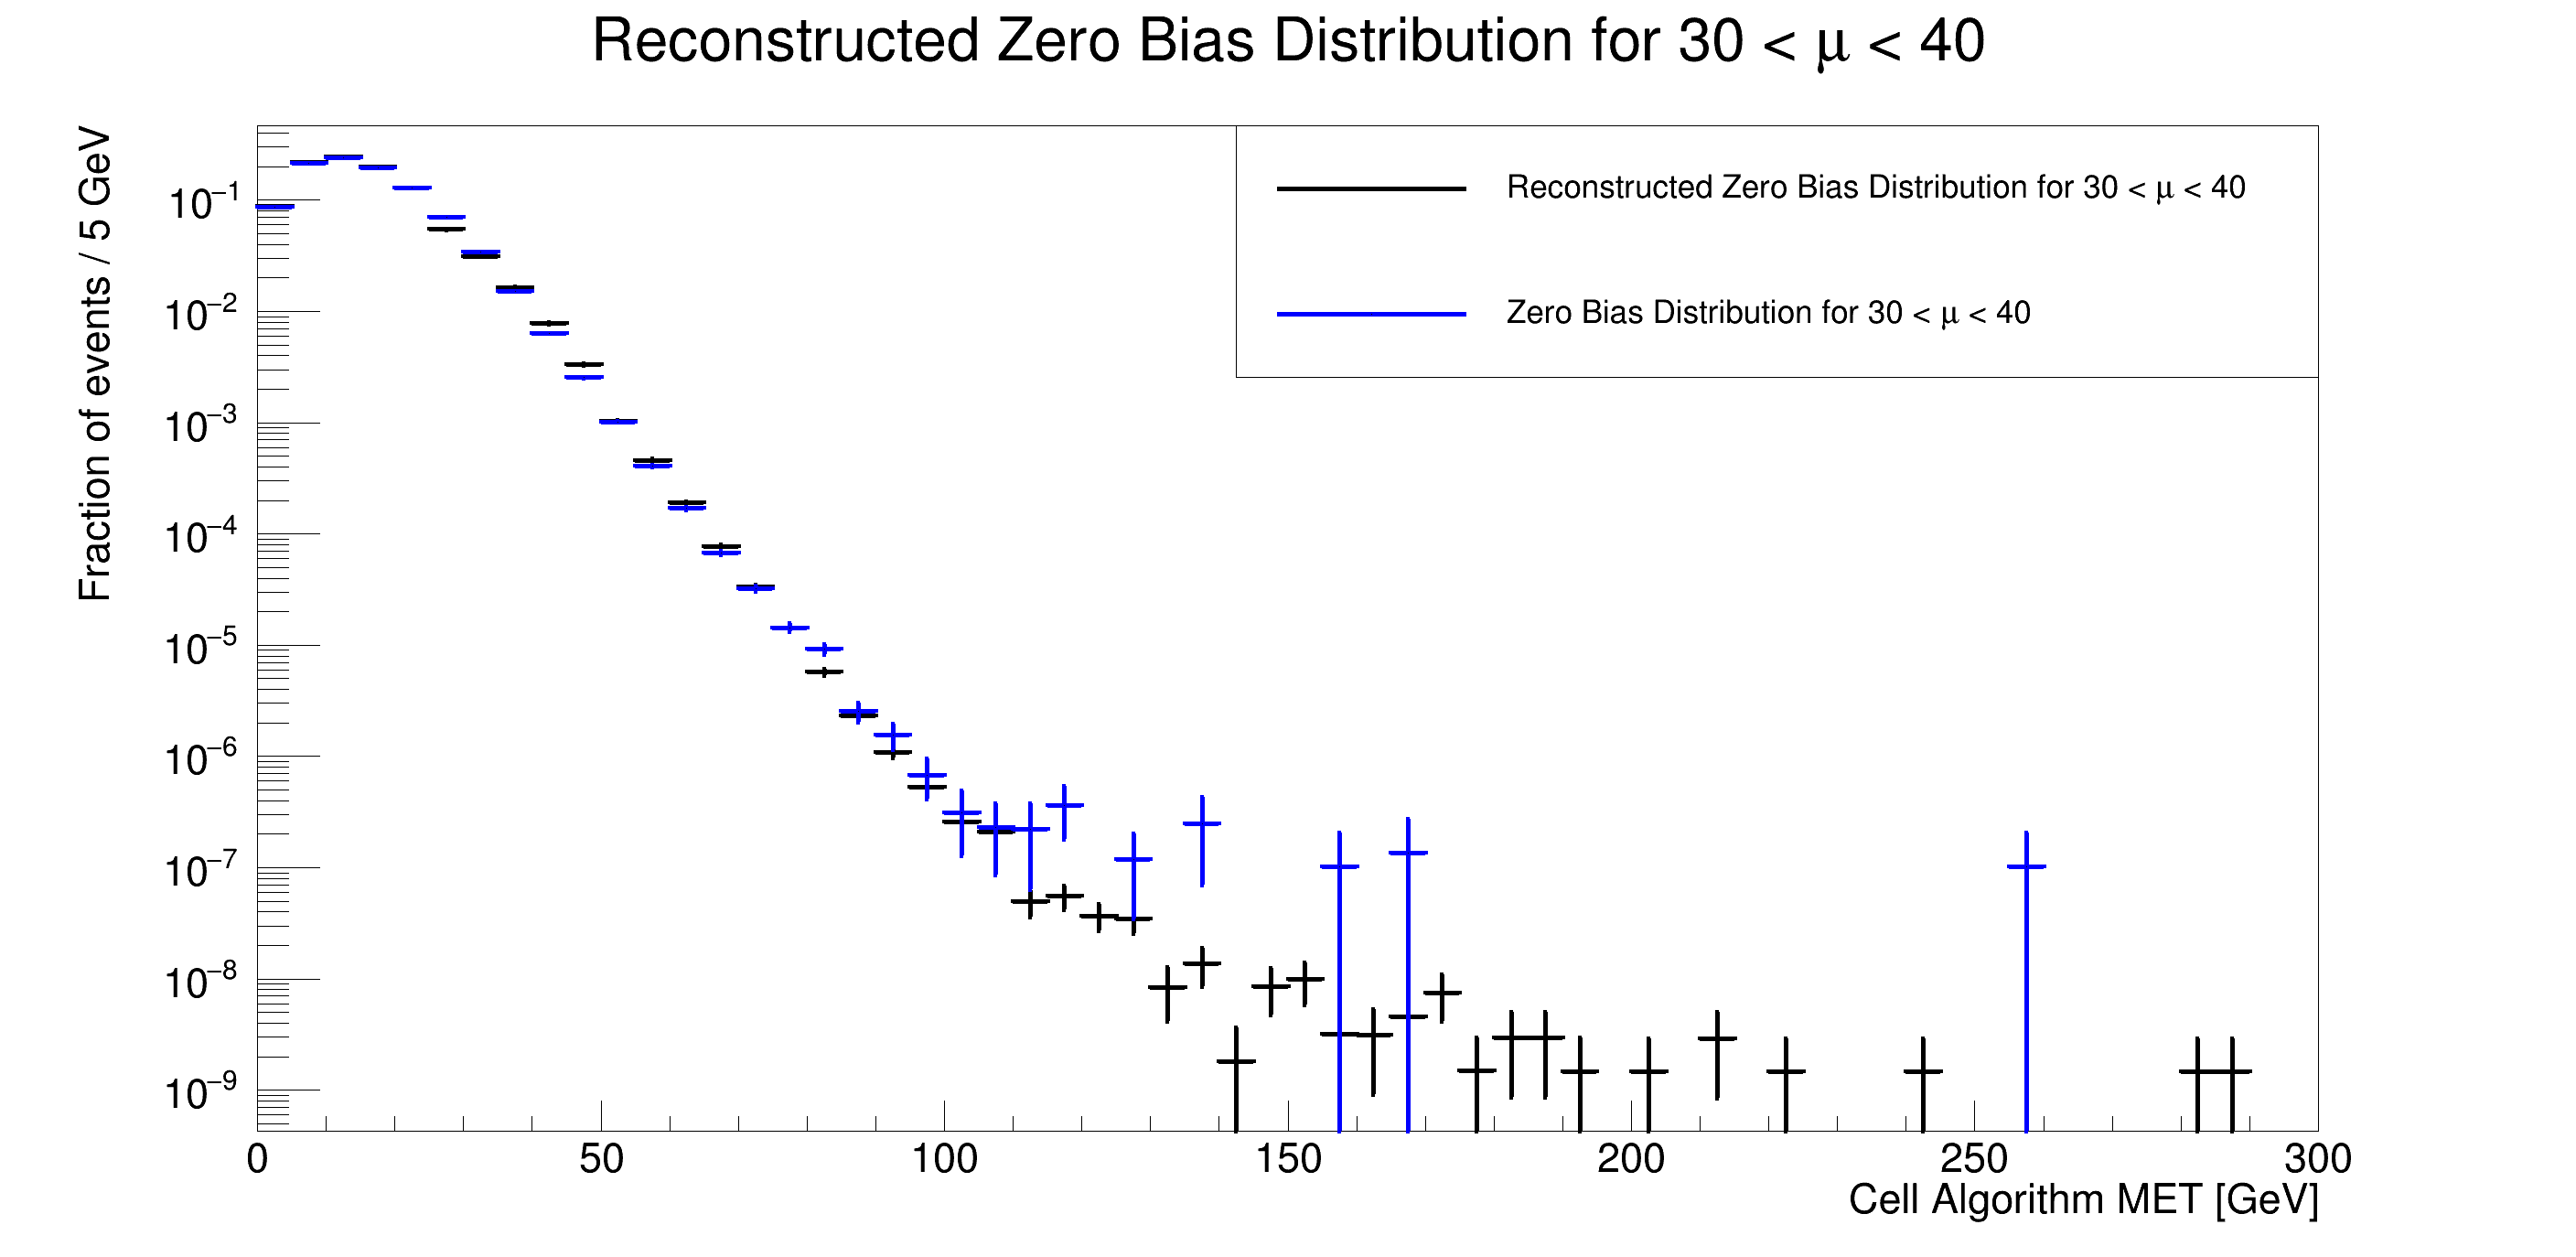
\includegraphics[height=2.65in,width=4.25in]{reconstructed_distributions/reconstructed_distribution_mubin_3}}
\end{frame}
\begin{frame}
		\framebox{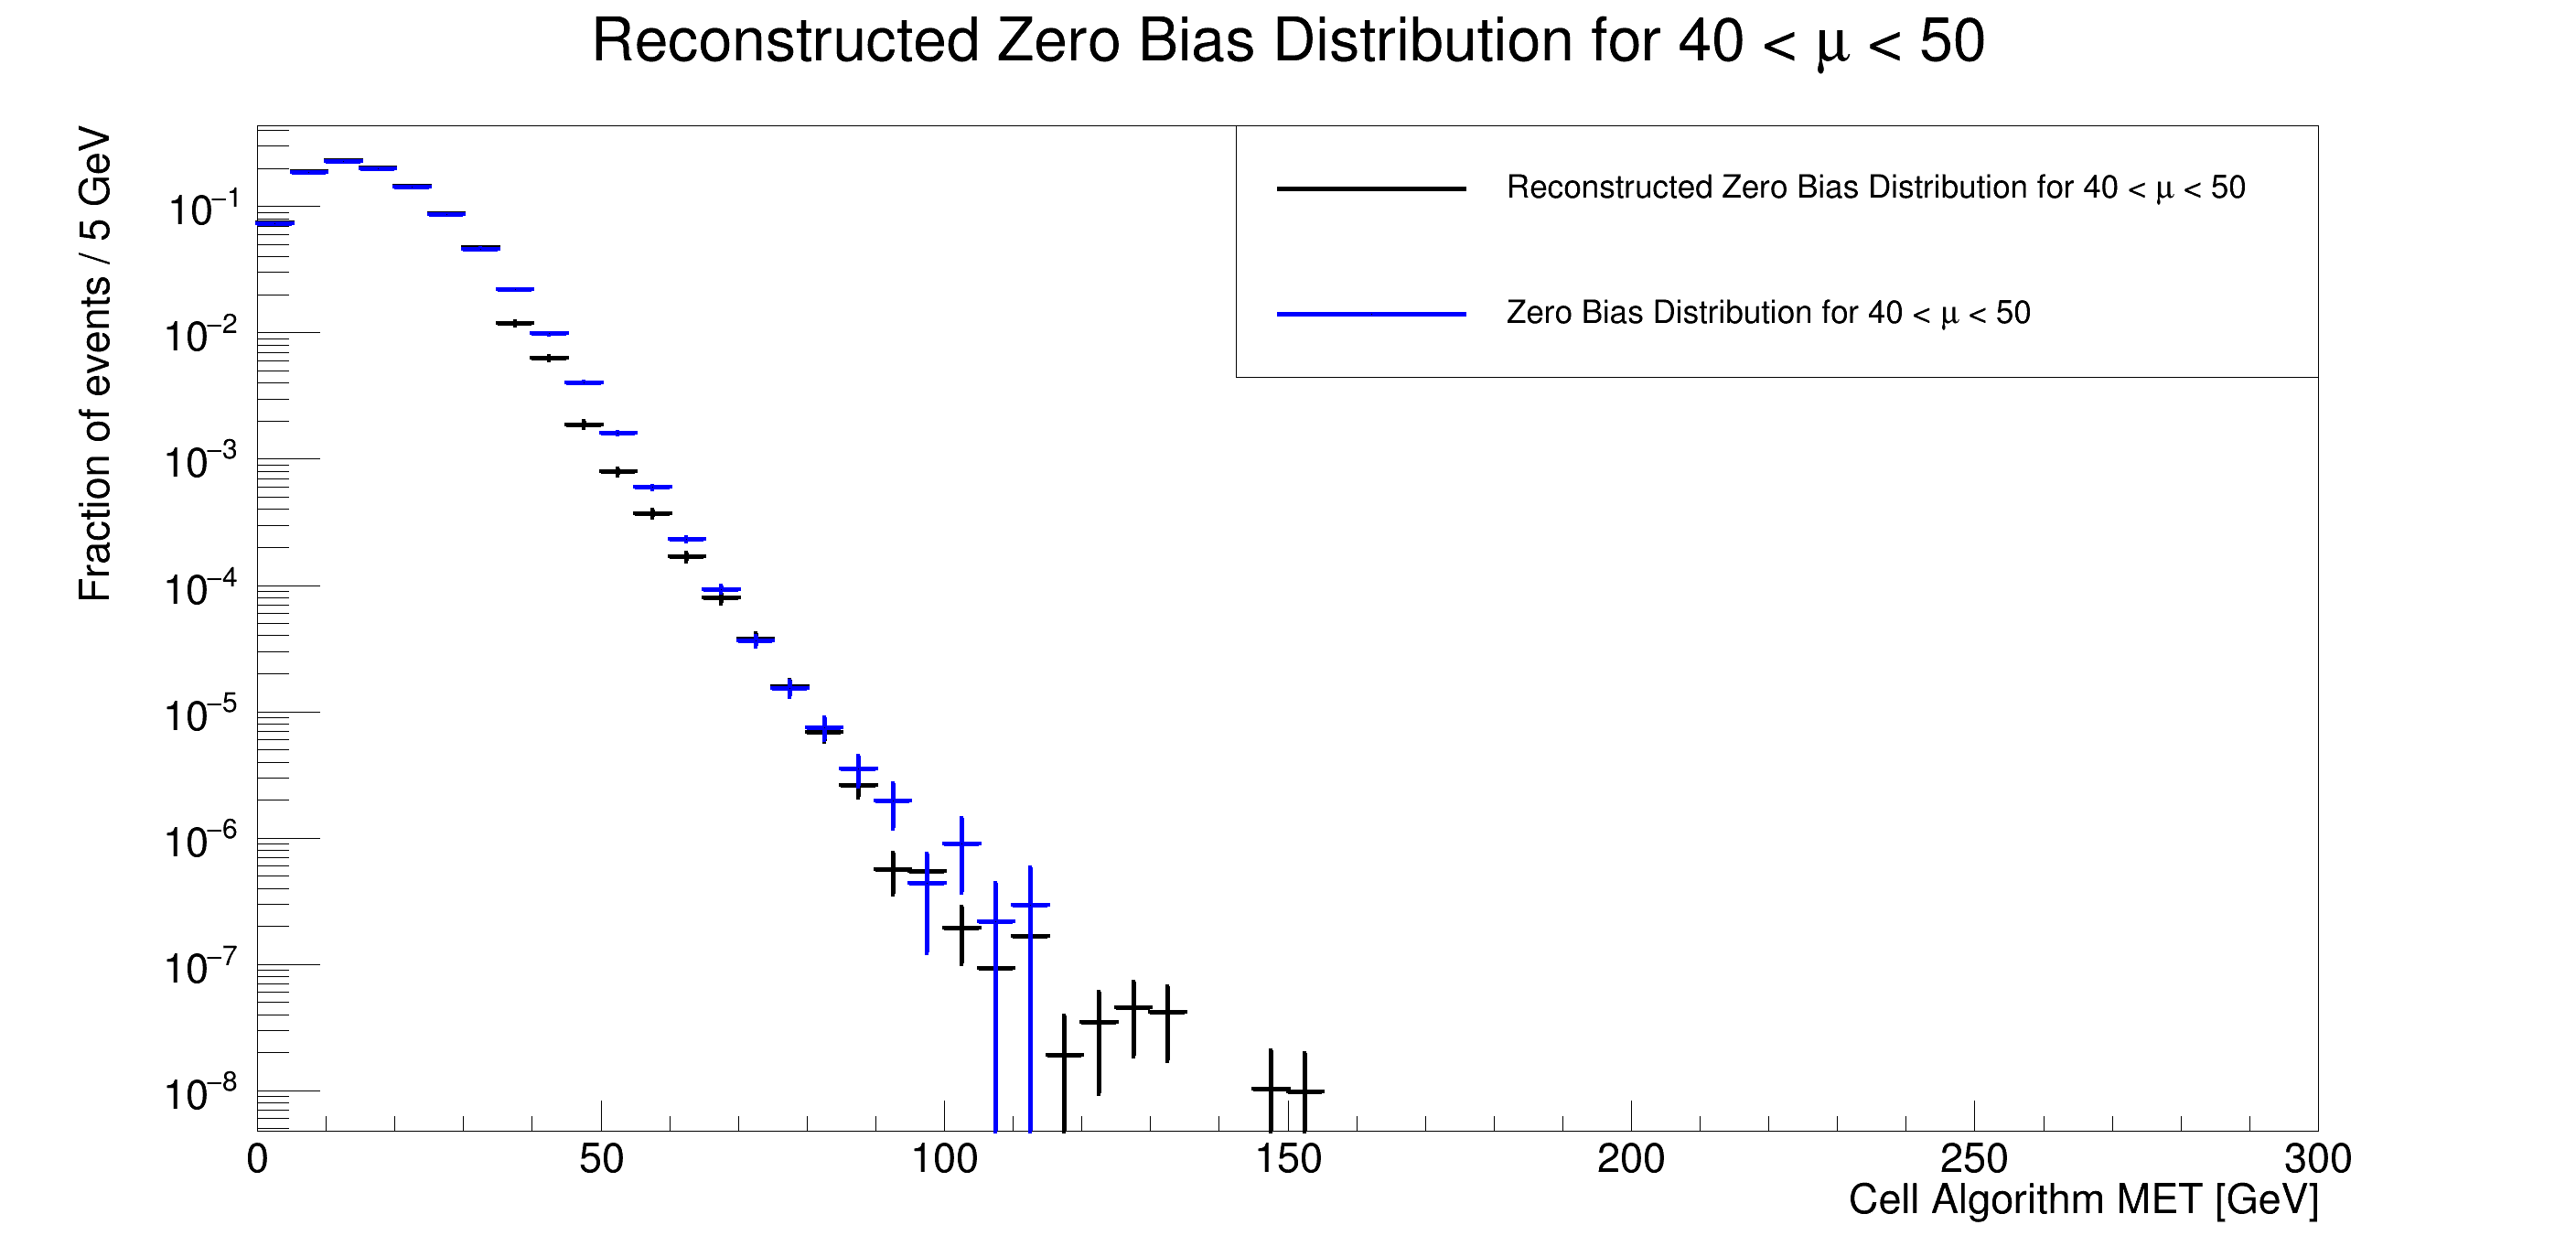
\includegraphics[height=2.65in,width=4.25in]{reconstructed_distributions/reconstructed_distribution_mubin_4}}
\end{frame}
\begin{frame}
		\framebox{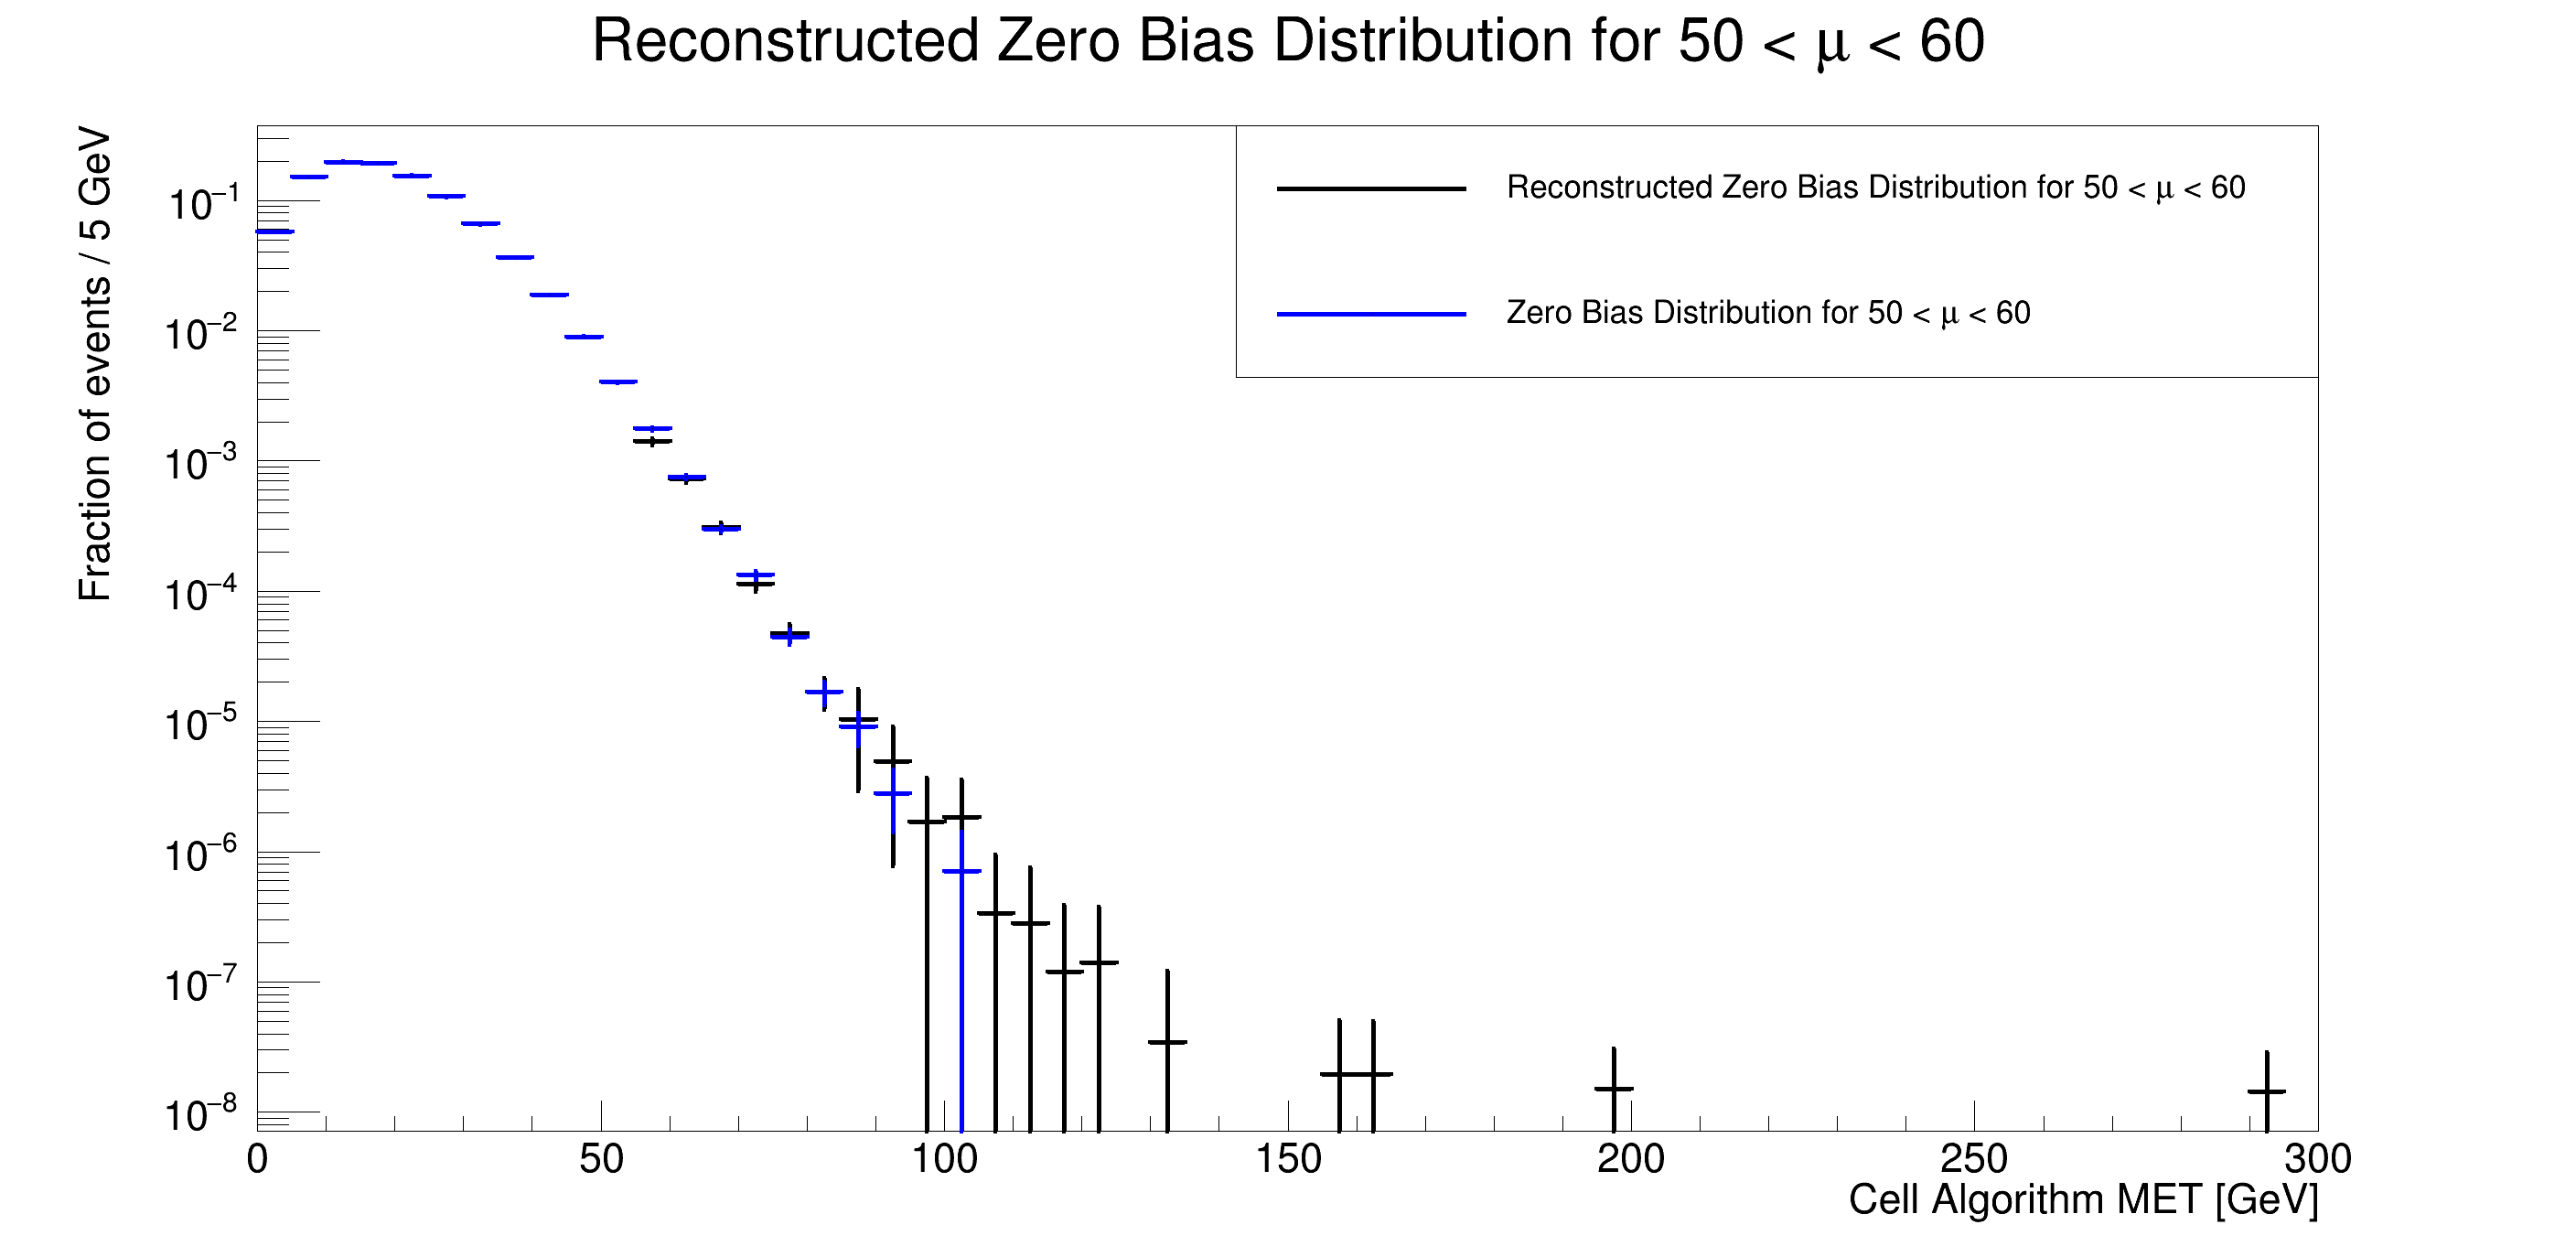
\includegraphics[height=2.65in,width=4.25in]{reconstructed_distributions/reconstructed_distribution_mubin_5}}
\end{frame}
\begin{frame}
		\framebox{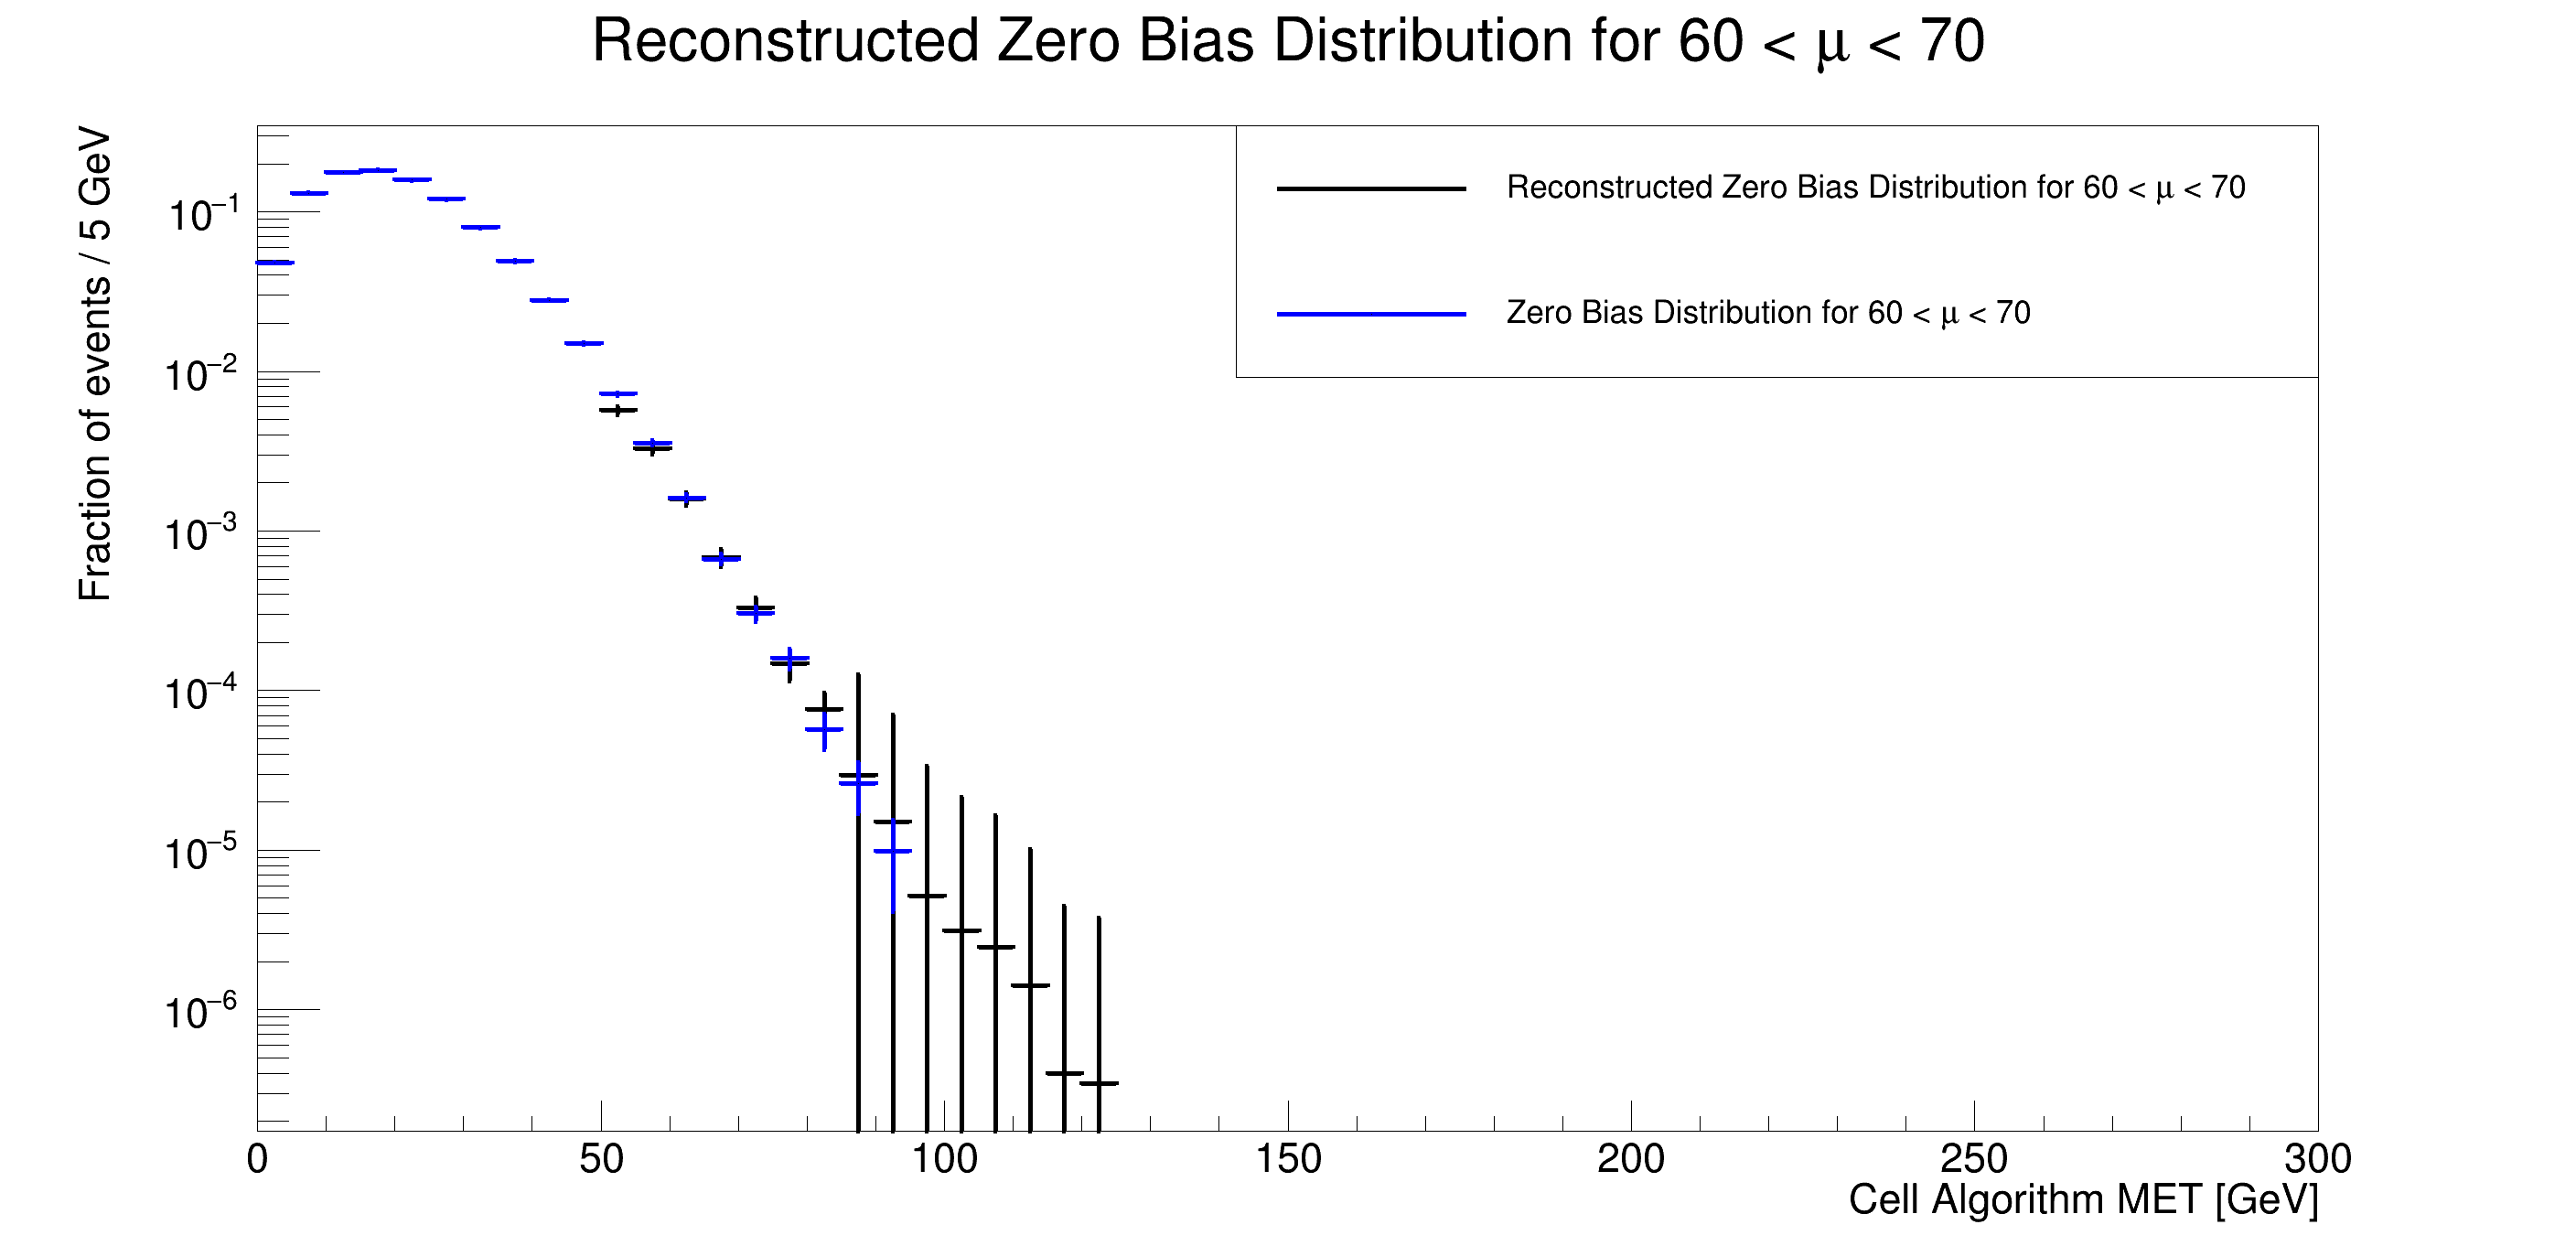
\includegraphics[height=2.65in,width=4.25in]{reconstructed_distributions/reconstructed_distribution_mubin_6}}
\end{frame}
\begin{frame}
\section{Appendix}
\LARGE{Appendix}
\end{frame}

\begin{frame}
        \frametitle{L1XE30 Efficiencies with respect to \texttt{HLTnoalg\_L1ZB} Data}
		\framebox{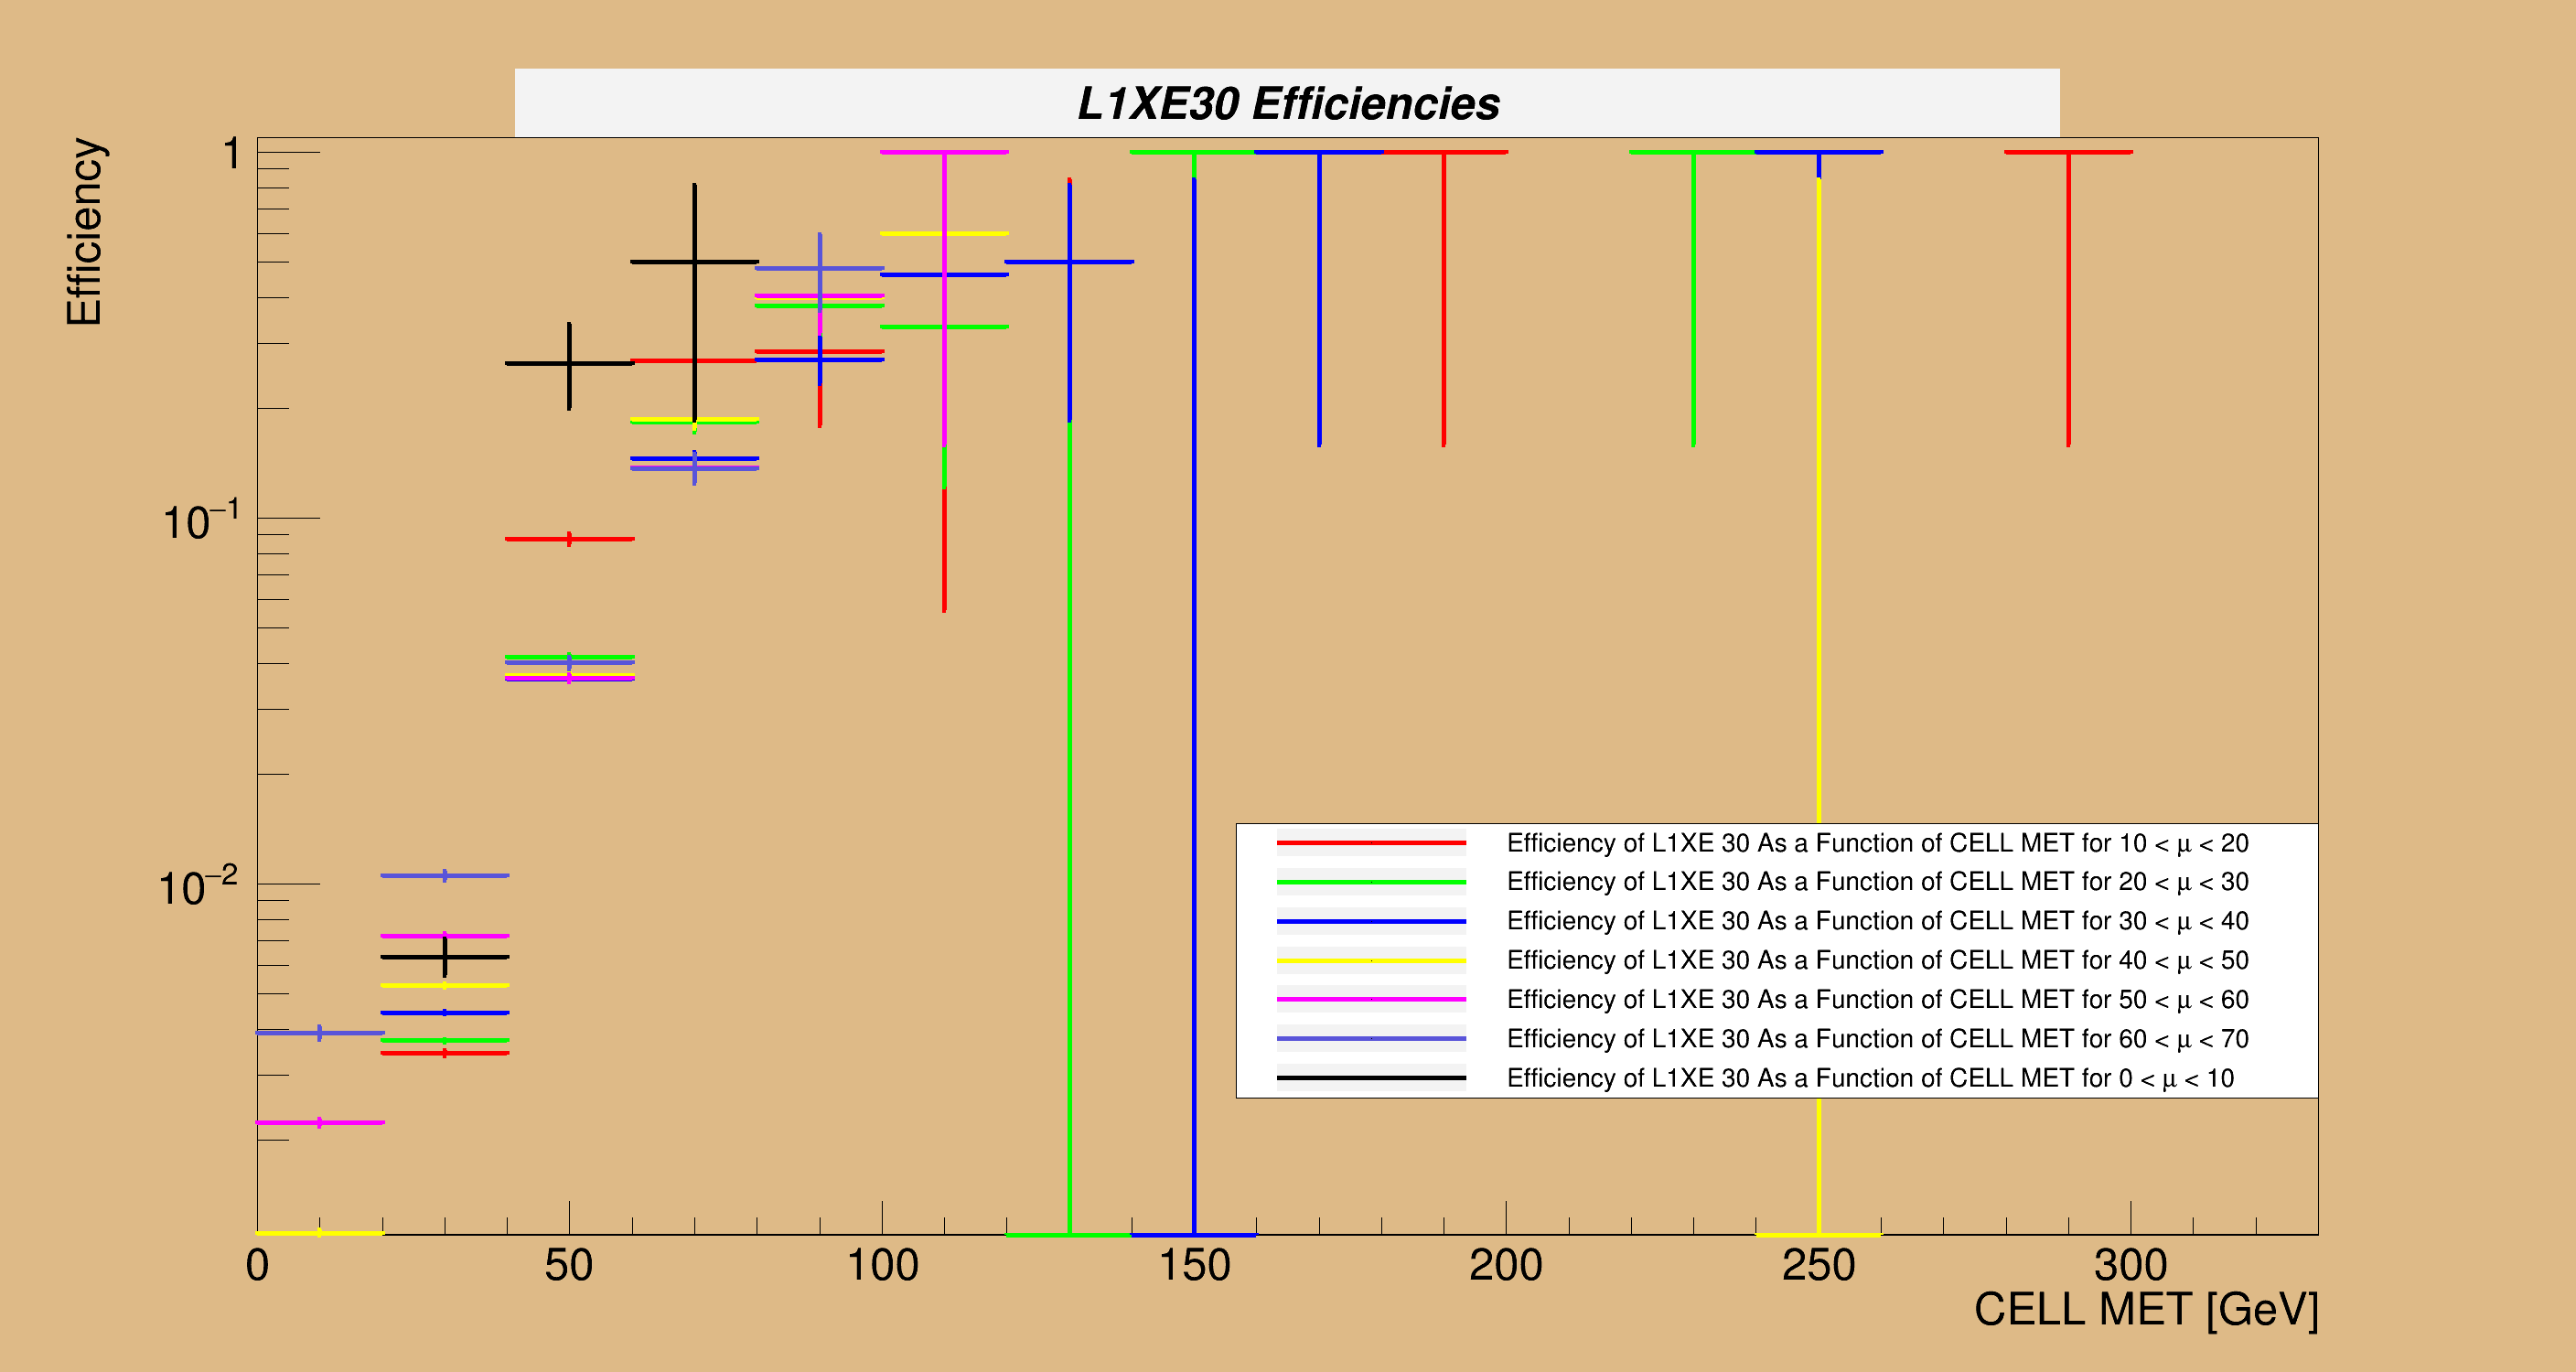
\includegraphics[height=2.65in,width=4.25in]{L1XE30Efficiency_Curves}}
\end{frame}
\begin{frame}
        \frametitle{L1XE30 Efficiency Fits with respect to \texttt{HLTnoalg\_L1ZB} Data}
		\framebox{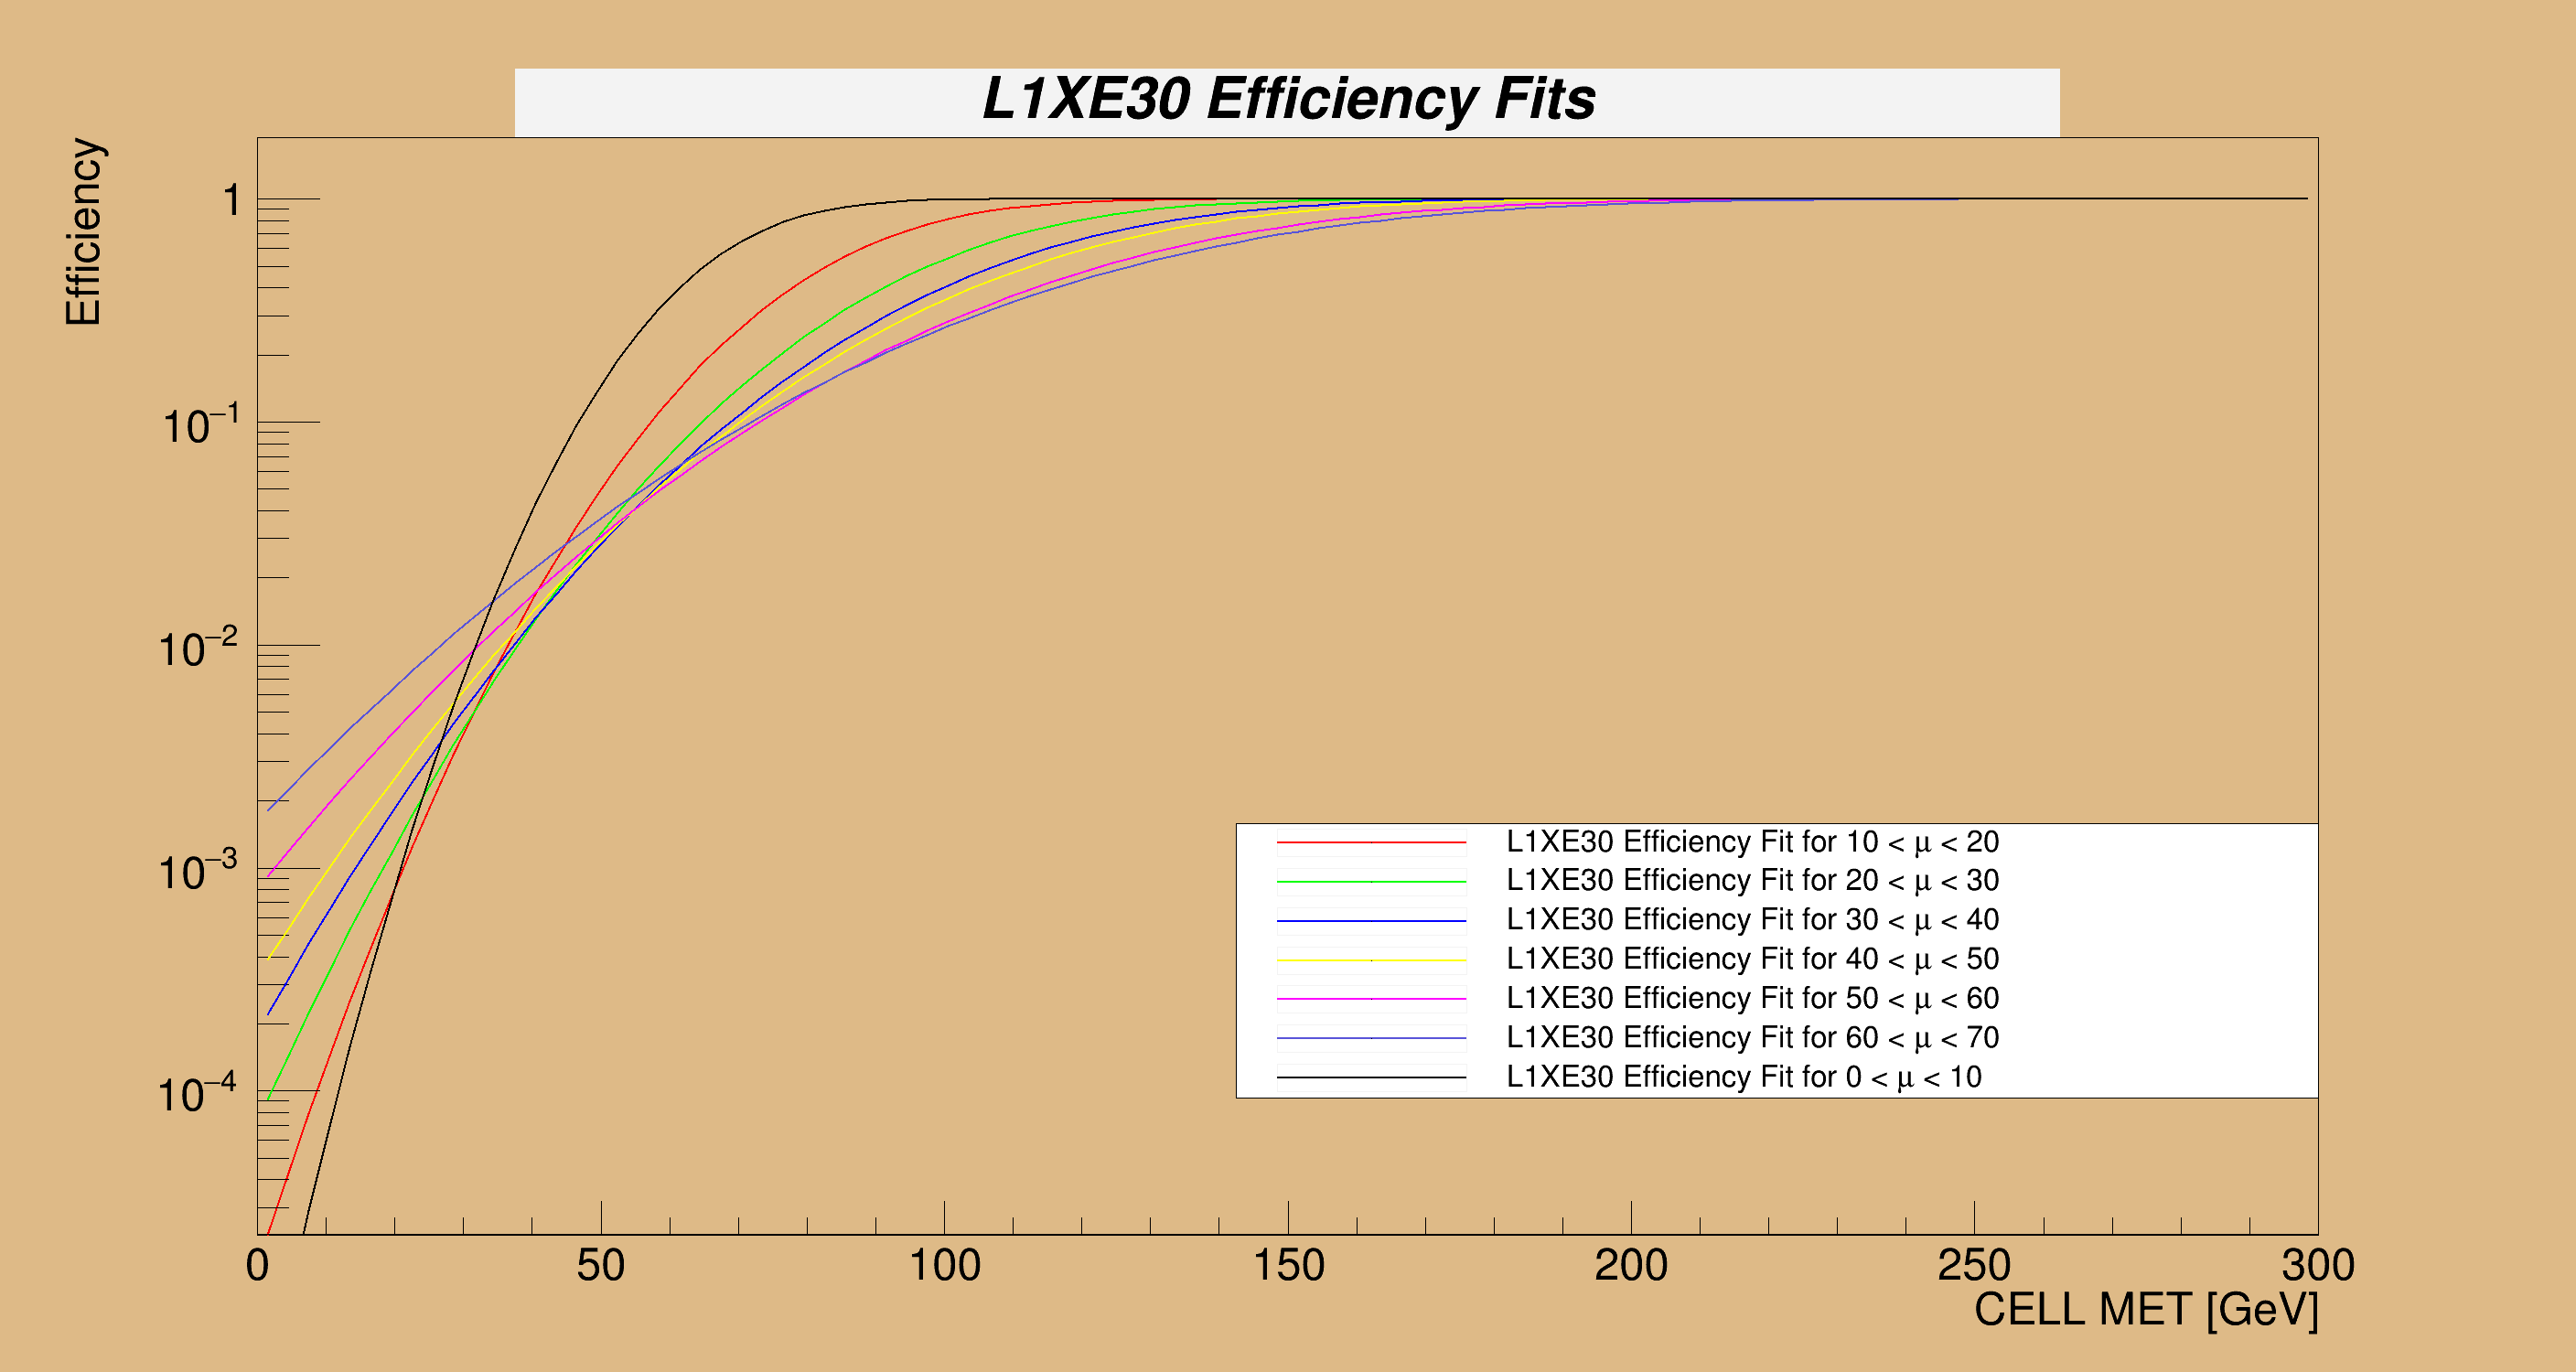
\includegraphics[height=2.65in,width=4.25in]{L1XE30Efficiency_Fits}}
\end{frame}
\begin{frame}
        \frametitle{L1XE50 Efficiencies with respect to \texttt{HLTnoalg\_L1XE30} Data}
		\framebox{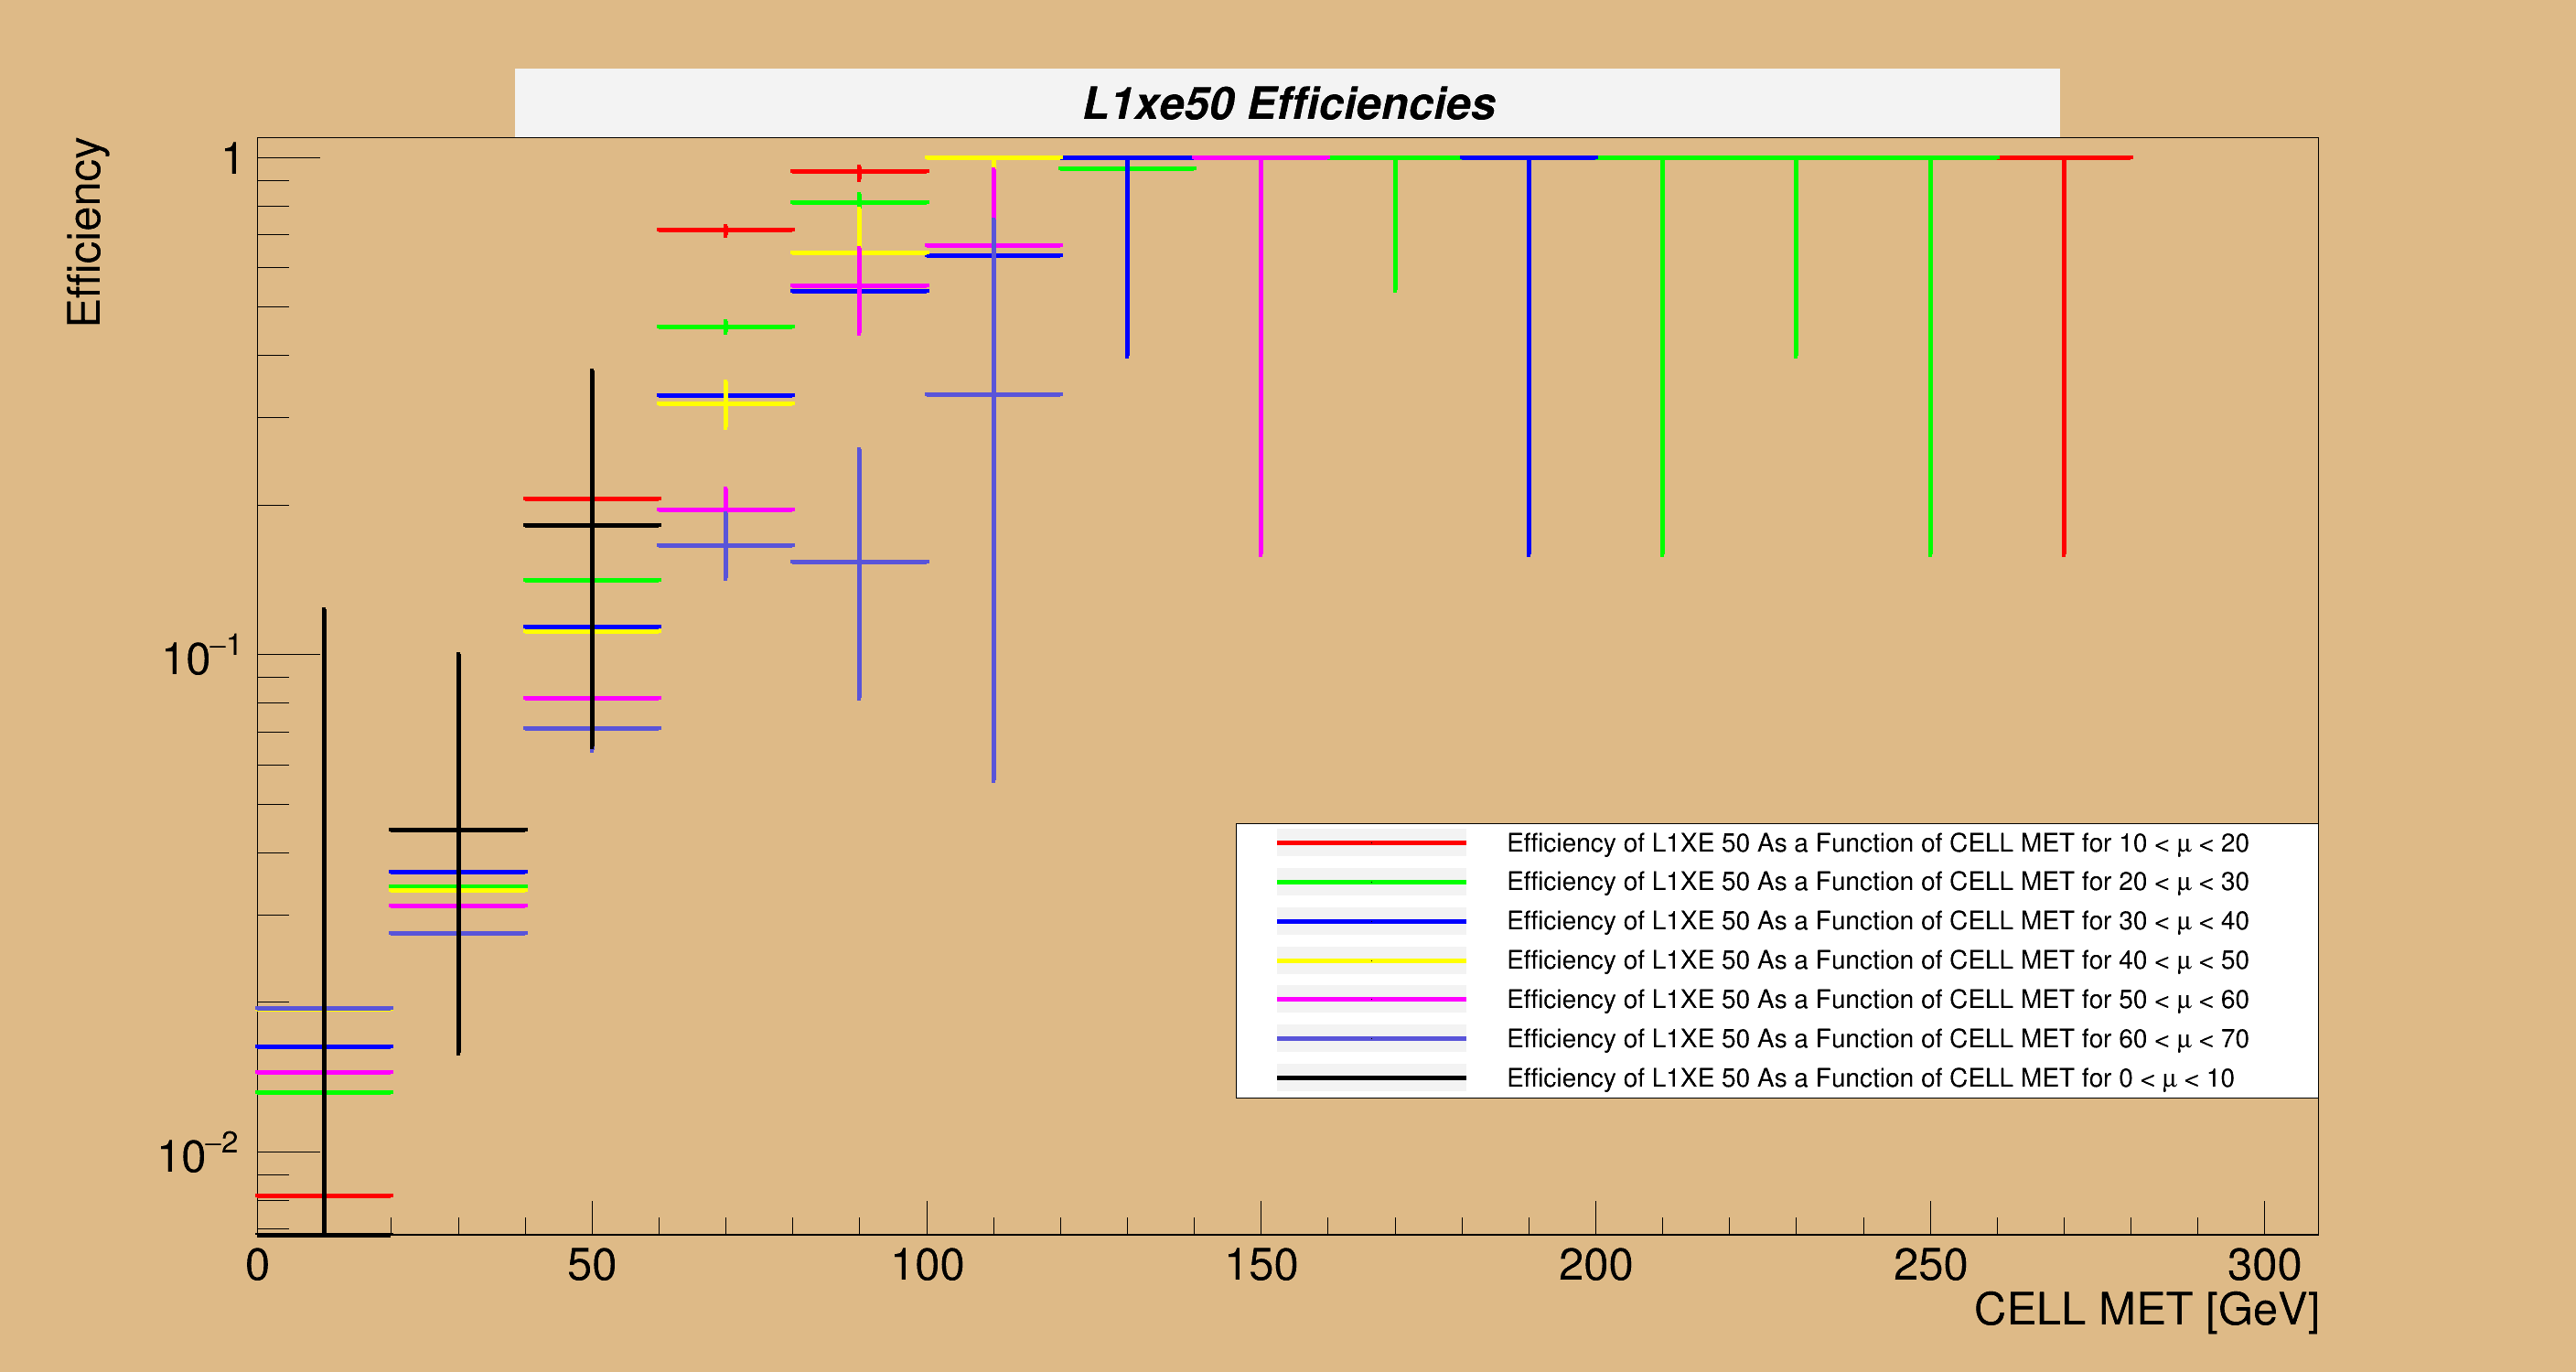
\includegraphics[height=2.65in,width=4.25in]{L1XE50Efficiency_Curves}}
\end{frame}
\begin{frame}
        \frametitle{L1XE50 Efficiency Fits with respect to \texttt{HLTnoalg\_L1XE30} Data}
		\framebox{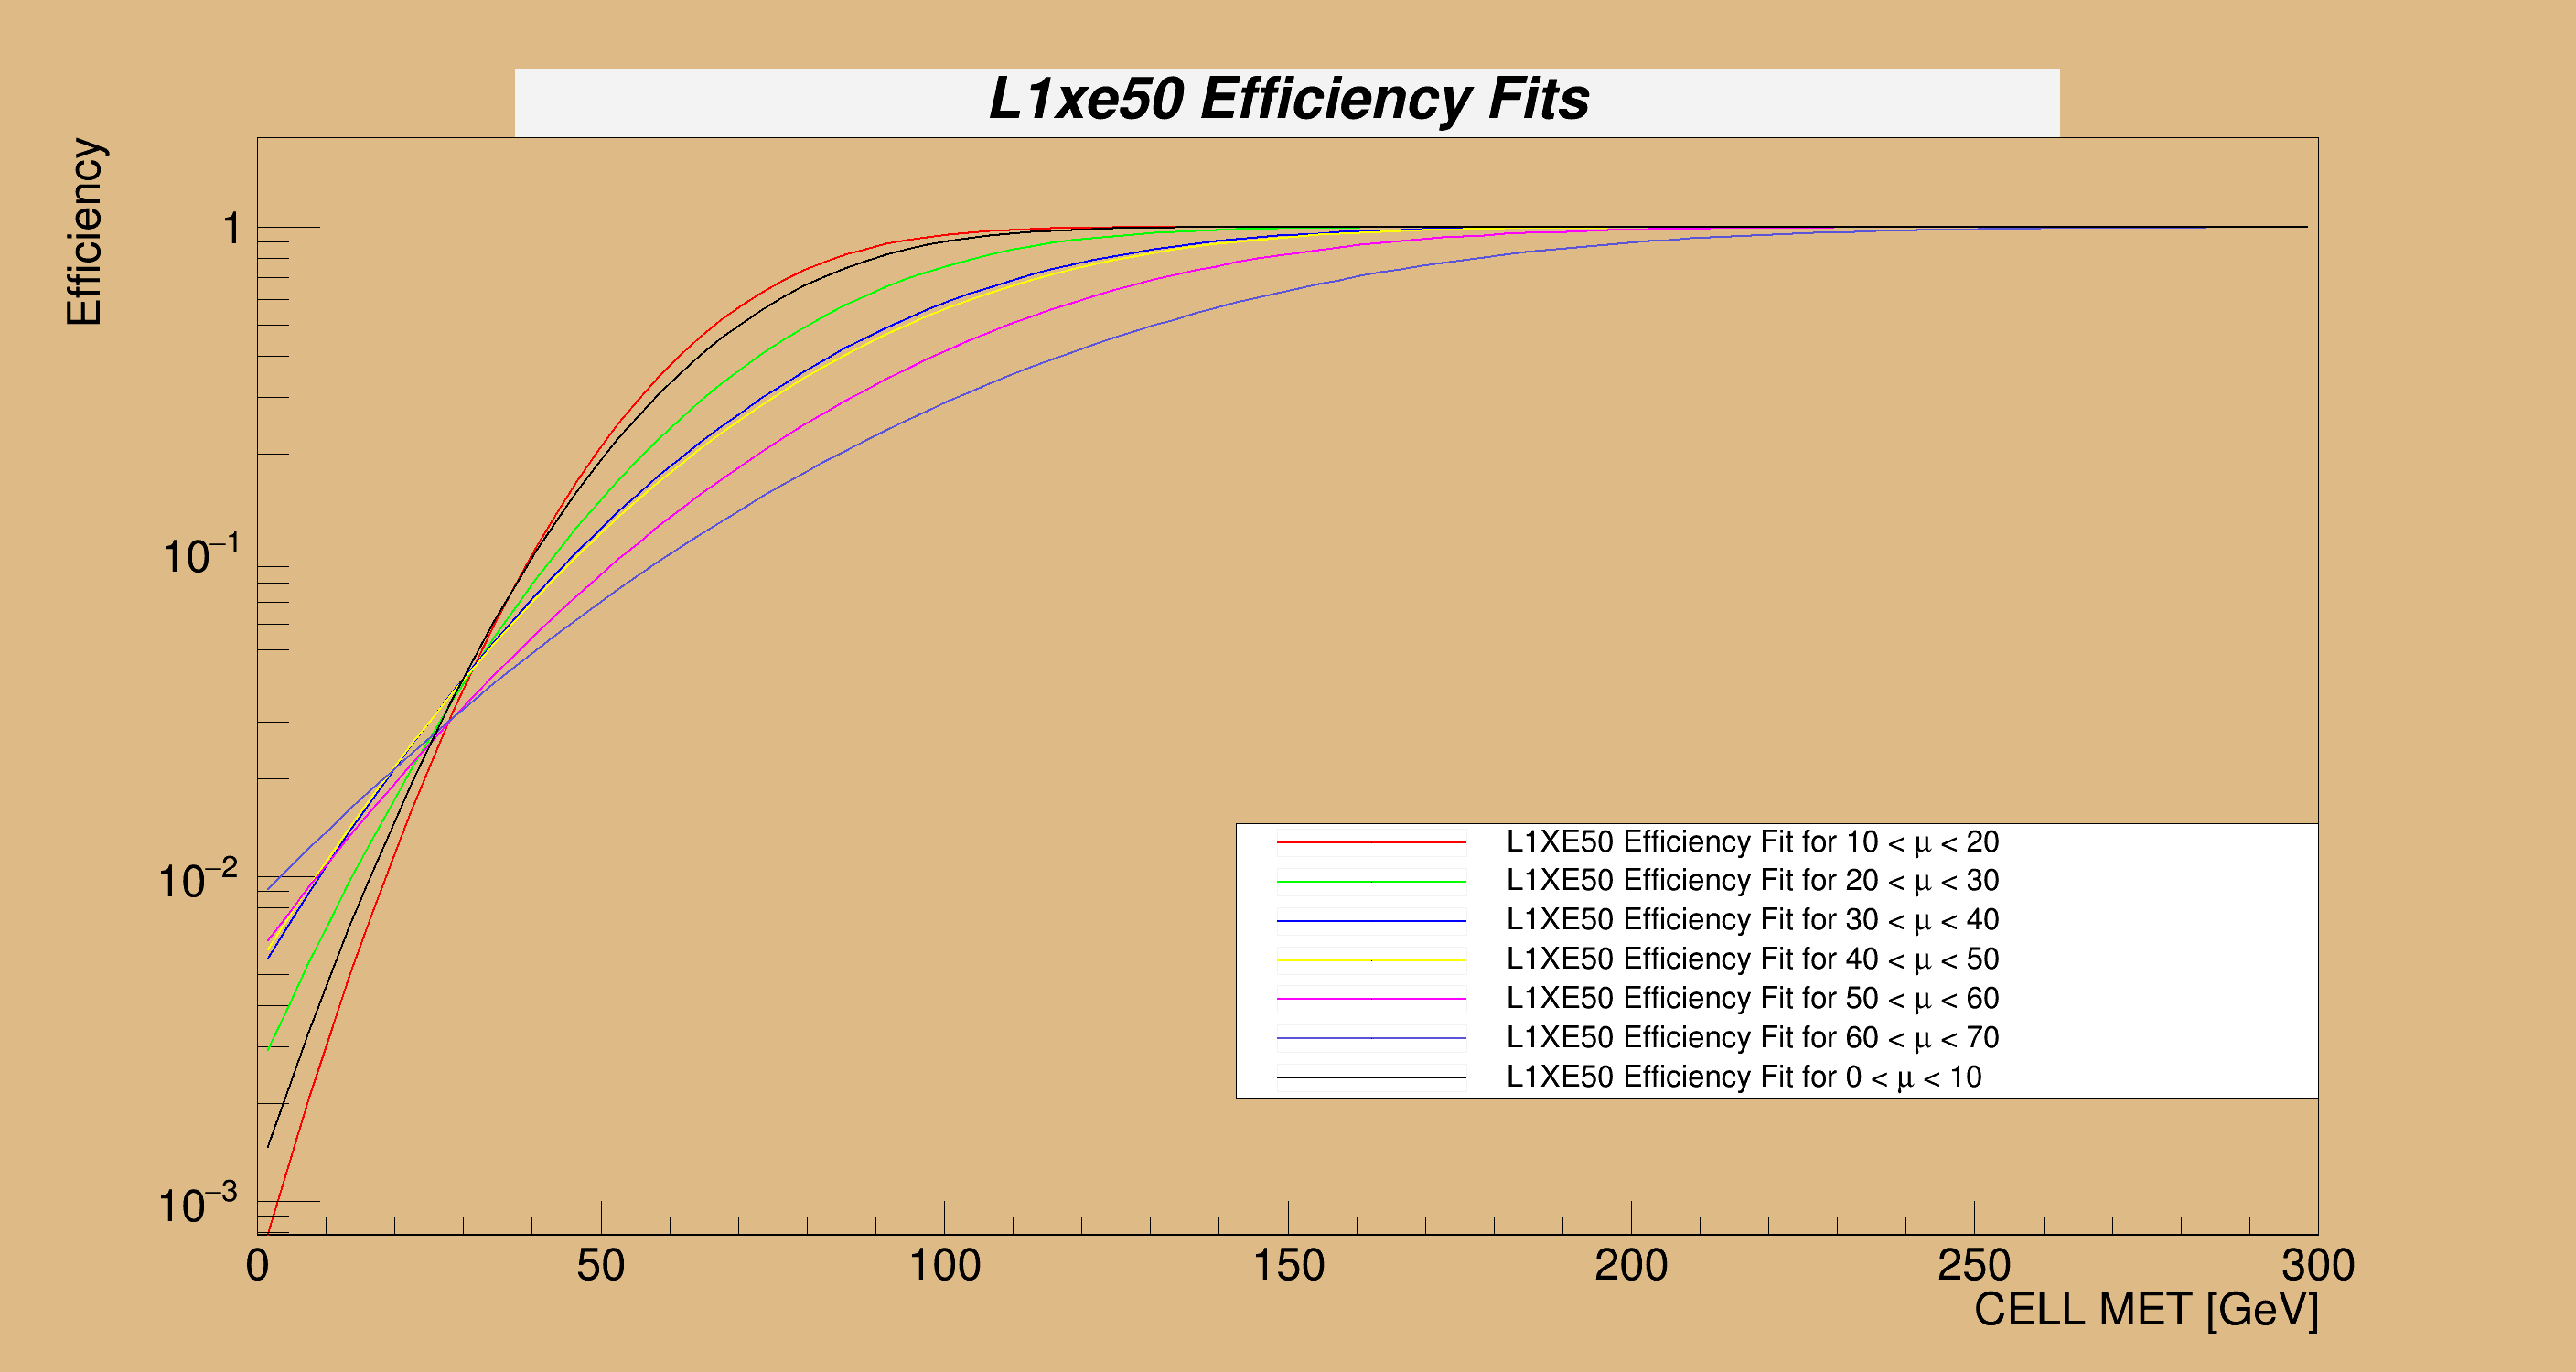
\includegraphics[height=2.65in,width=4.25in]{L1XE50Efficiency_Fits}}
\end{frame}
% HLTNOALG L1XE30 Plots
\begin{frame}
        \frametitle{\texttt{HLTnoalg\_L1XE30} Plot for $0<\mu<10$}
        \framebox{\includegraphics[height=2.65in,width=4.25in]{hlt_noalg_l1xe30_plots/hlt_noalg_L1XE30_dist_mubin_0}}
\end{frame}
\begin{frame}
        \frametitle{\texttt{HLTnoalg\_L1XE30} Plot for $10<\mu<20$}
        \framebox{\includegraphics[height=2.65in,width=4.25in]{hlt_noalg_l1xe30_plots/hlt_noalg_L1XE30_dist_mubin_1}}
\end{frame}
\begin{frame}
        \frametitle{\texttt{HLTnoalg\_L1XE30} Plot for $20<\mu<30$}
        \framebox{\includegraphics[height=2.65in,width=4.25in]{hlt_noalg_l1xe30_plots/hlt_noalg_L1XE30_dist_mubin_2}}
\end{frame}
\begin{frame}
        \frametitle{\texttt{HLTnoalg\_L1XE30} Plot for $30<\mu<40$}
        \framebox{\includegraphics[height=2.65in,width=4.25in]{hlt_noalg_l1xe30_plots/hlt_noalg_L1XE30_dist_mubin_3}}
\end{frame}
\begin{frame}
        \frametitle{\texttt{HLTnoalg\_L1XE30} Plot for $40<\mu<50$}
        \framebox{\includegraphics[height=2.65in,width=4.25in]{hlt_noalg_l1xe30_plots/hlt_noalg_L1XE30_dist_mubin_4}}
\end{frame}
\begin{frame}
        \frametitle{\texttt{HLTnoalg\_L1XE30} Plot for $50<\mu<60$}
        \framebox{\includegraphics[height=2.65in,width=4.25in]{hlt_noalg_l1xe30_plots/hlt_noalg_L1XE30_dist_mubin_5}}
\end{frame}
\begin{frame}
        \frametitle{\texttt{HLTnoalg\_L1XE30} Plot for $60<\mu<70$}
        \framebox{\includegraphics[height=2.65in,width=4.25in]{hlt_noalg_l1xe30_plots/hlt_noalg_L1XE30_dist_mubin_6}}
\end{frame}
% HLTNOALG L1XE50 Plots
\begin{frame}
        \frametitle{\texttt{HLTnoalg\_L1XE50} Plot for $0<\mu<10$}
        \framebox{\includegraphics[height=2.65in,width=4.25in]{hlt_noalg_l1xe50_plots/hlt_noalg_L1XE50_dist_mubin_0}}
\end{frame}
\begin{frame}
        \frametitle{\texttt{HLTnoalg\_L1XE50} Plot for $10<\mu<20$}
        \framebox{\includegraphics[height=2.65in,width=4.25in]{hlt_noalg_l1xe50_plots/hlt_noalg_L1XE50_dist_mubin_1}}
\end{frame}
\begin{frame}
        \frametitle{\texttt{HLTnoalg\_L1XE50} Plot for $20<\mu<30$}
        \framebox{\includegraphics[height=2.65in,width=4.25in]{hlt_noalg_l1xe50_plots/hlt_noalg_L1XE50_dist_mubin_2}}
\end{frame}
\begin{frame}
        \frametitle{\texttt{HLTnoalg\_L1XE50} Plot for $30<\mu<40$}
        \framebox{\includegraphics[height=2.65in,width=4.25in]{hlt_noalg_l1xe50_plots/hlt_noalg_L1XE50_dist_mubin_3}}
\end{frame}
\begin{frame}
        \frametitle{\texttt{HLTnoalg\_L1XE50} Plot for $40<\mu<50$}
        \framebox{\includegraphics[height=2.65in,width=4.25in]{hlt_noalg_l1xe50_plots/hlt_noalg_L1XE50_dist_mubin_4}}
\end{frame}
\begin{frame}
        \frametitle{\texttt{HLTnoalg\_L1XE50} Plot for $50<\mu<60$}
        \framebox{\includegraphics[height=2.65in,width=4.25in]{hlt_noalg_l1xe50_plots/hlt_noalg_L1XE50_dist_mubin_5}}
\end{frame}
\begin{frame}
        \frametitle{\texttt{HLTnoalg\_L1XE50} Plot for $60<\mu<70$}
        \framebox{\includegraphics[height=2.65in,width=4.25in]{hlt_noalg_l1xe50_plots/hlt_noalg_L1XE50_dist_mubin_6}}
\end{frame}
% L1XE30 Efficiency Curves
\begin{frame}
        \frametitle{L1XE30 Efficiency Curve Plot for $0<\mu<10$}
        \framebox{\includegraphics[height=2.65in,width=4.25in]{l1xe30_efficiencies/L1XE30Efficiency_mu_between_0_10}}
\end{frame}
\begin{frame}
        \frametitle{L1XE30 Efficiency Curve Plot for $10<\mu<20$}
        \framebox{\includegraphics[height=2.65in,width=4.25in]{l1xe30_efficiencies/L1XE30Efficiency_mu_between_10_20}}
\end{frame}
\begin{frame}
        \frametitle{L1XE30 Efficiency Curve Plot for $20<\mu<30$}
        \framebox{\includegraphics[height=2.65in,width=4.25in]{l1xe30_efficiencies/L1XE30Efficiency_mu_between_20_30}}
\end{frame}
\begin{frame}
        \frametitle{L1XE30 Efficiency Curve Plot for $30<\mu<40$}
        \framebox{\includegraphics[height=2.65in,width=4.25in]{l1xe30_efficiencies/L1XE30Efficiency_mu_between_30_40}}
\end{frame}
\begin{frame}
        \frametitle{L1XE30 Efficiency Curve Plot for $40<\mu<50$}
        \framebox{\includegraphics[height=2.65in,width=4.25in]{l1xe30_efficiencies/L1XE30Efficiency_mu_between_40_50}}
\end{frame}
\begin{frame}
        \frametitle{L1XE30 Efficiency Curve Plot for $50<\mu<60$}
        \framebox{\includegraphics[height=2.65in,width=4.25in]{l1xe30_efficiencies/L1XE30Efficiency_mu_between_50_60}}
\end{frame}
\begin{frame}
        \frametitle{L1XE30 Efficiency Curve Plot for $60<\mu<70$}
        \framebox{\includegraphics[height=2.65in,width=4.25in]{l1xe30_efficiencies/L1XE30Efficiency_mu_between_60_70}}
\end{frame}
% L1XE50 Efficiency Curves
\begin{frame}
        \frametitle{L1XE50 Efficiency Curve Plot for $0<\mu<10$}
        \framebox{\includegraphics[height=2.65in,width=4.25in]{l1xe50_efficiencies/L1XE50Efficiency_mu_between_0_10}}
\end{frame}
\begin{frame}
        \frametitle{L1XE50 Efficiency Curve Plot for $10<\mu<20$}
        \framebox{\includegraphics[height=2.65in,width=4.25in]{l1xe50_efficiencies/L1XE50Efficiency_mu_between_10_20}}
\end{frame}
\begin{frame}
        \frametitle{L1XE50 Efficiency Curve Plot for $20<\mu<30$}
        \framebox{\includegraphics[height=2.65in,width=4.25in]{l1xe50_efficiencies/L1XE50Efficiency_mu_between_20_30}}
\end{frame}
\begin{frame}
        \frametitle{L1XE50 Efficiency Curve Plot for $30<\mu<40$}
        \framebox{\includegraphics[height=2.65in,width=4.25in]{l1xe50_efficiencies/L1XE50Efficiency_mu_between_30_40}}
\end{frame}
\begin{frame}
        \frametitle{L1XE50 Efficiency Curve Plot for $40<\mu<50$}
        \framebox{\includegraphics[height=2.65in,width=4.25in]{l1xe50_efficiencies/L1XE50Efficiency_mu_between_40_50}}
\end{frame}
\begin{frame}
        \frametitle{L1XE50 Efficiency Curve Plot for $50<\mu<60$}
        \framebox{\includegraphics[height=2.65in,width=4.25in]{l1xe50_efficiencies/L1XE50Efficiency_mu_between_50_60}}
\end{frame}
\begin{frame}
        \frametitle{L1XE50 Efficiency Curve Plot for $60<\mu<70$}
        \framebox{\includegraphics[height=2.65in,width=4.25in]{l1xe50_efficiencies/L1XE50Efficiency_mu_between_60_70}}
\end{frame}
% UNBIASED DISTRIBUTIONS
\begin{frame}
        \frametitle{Unbiased Distributions for $0<\mu<10$}
        \framebox{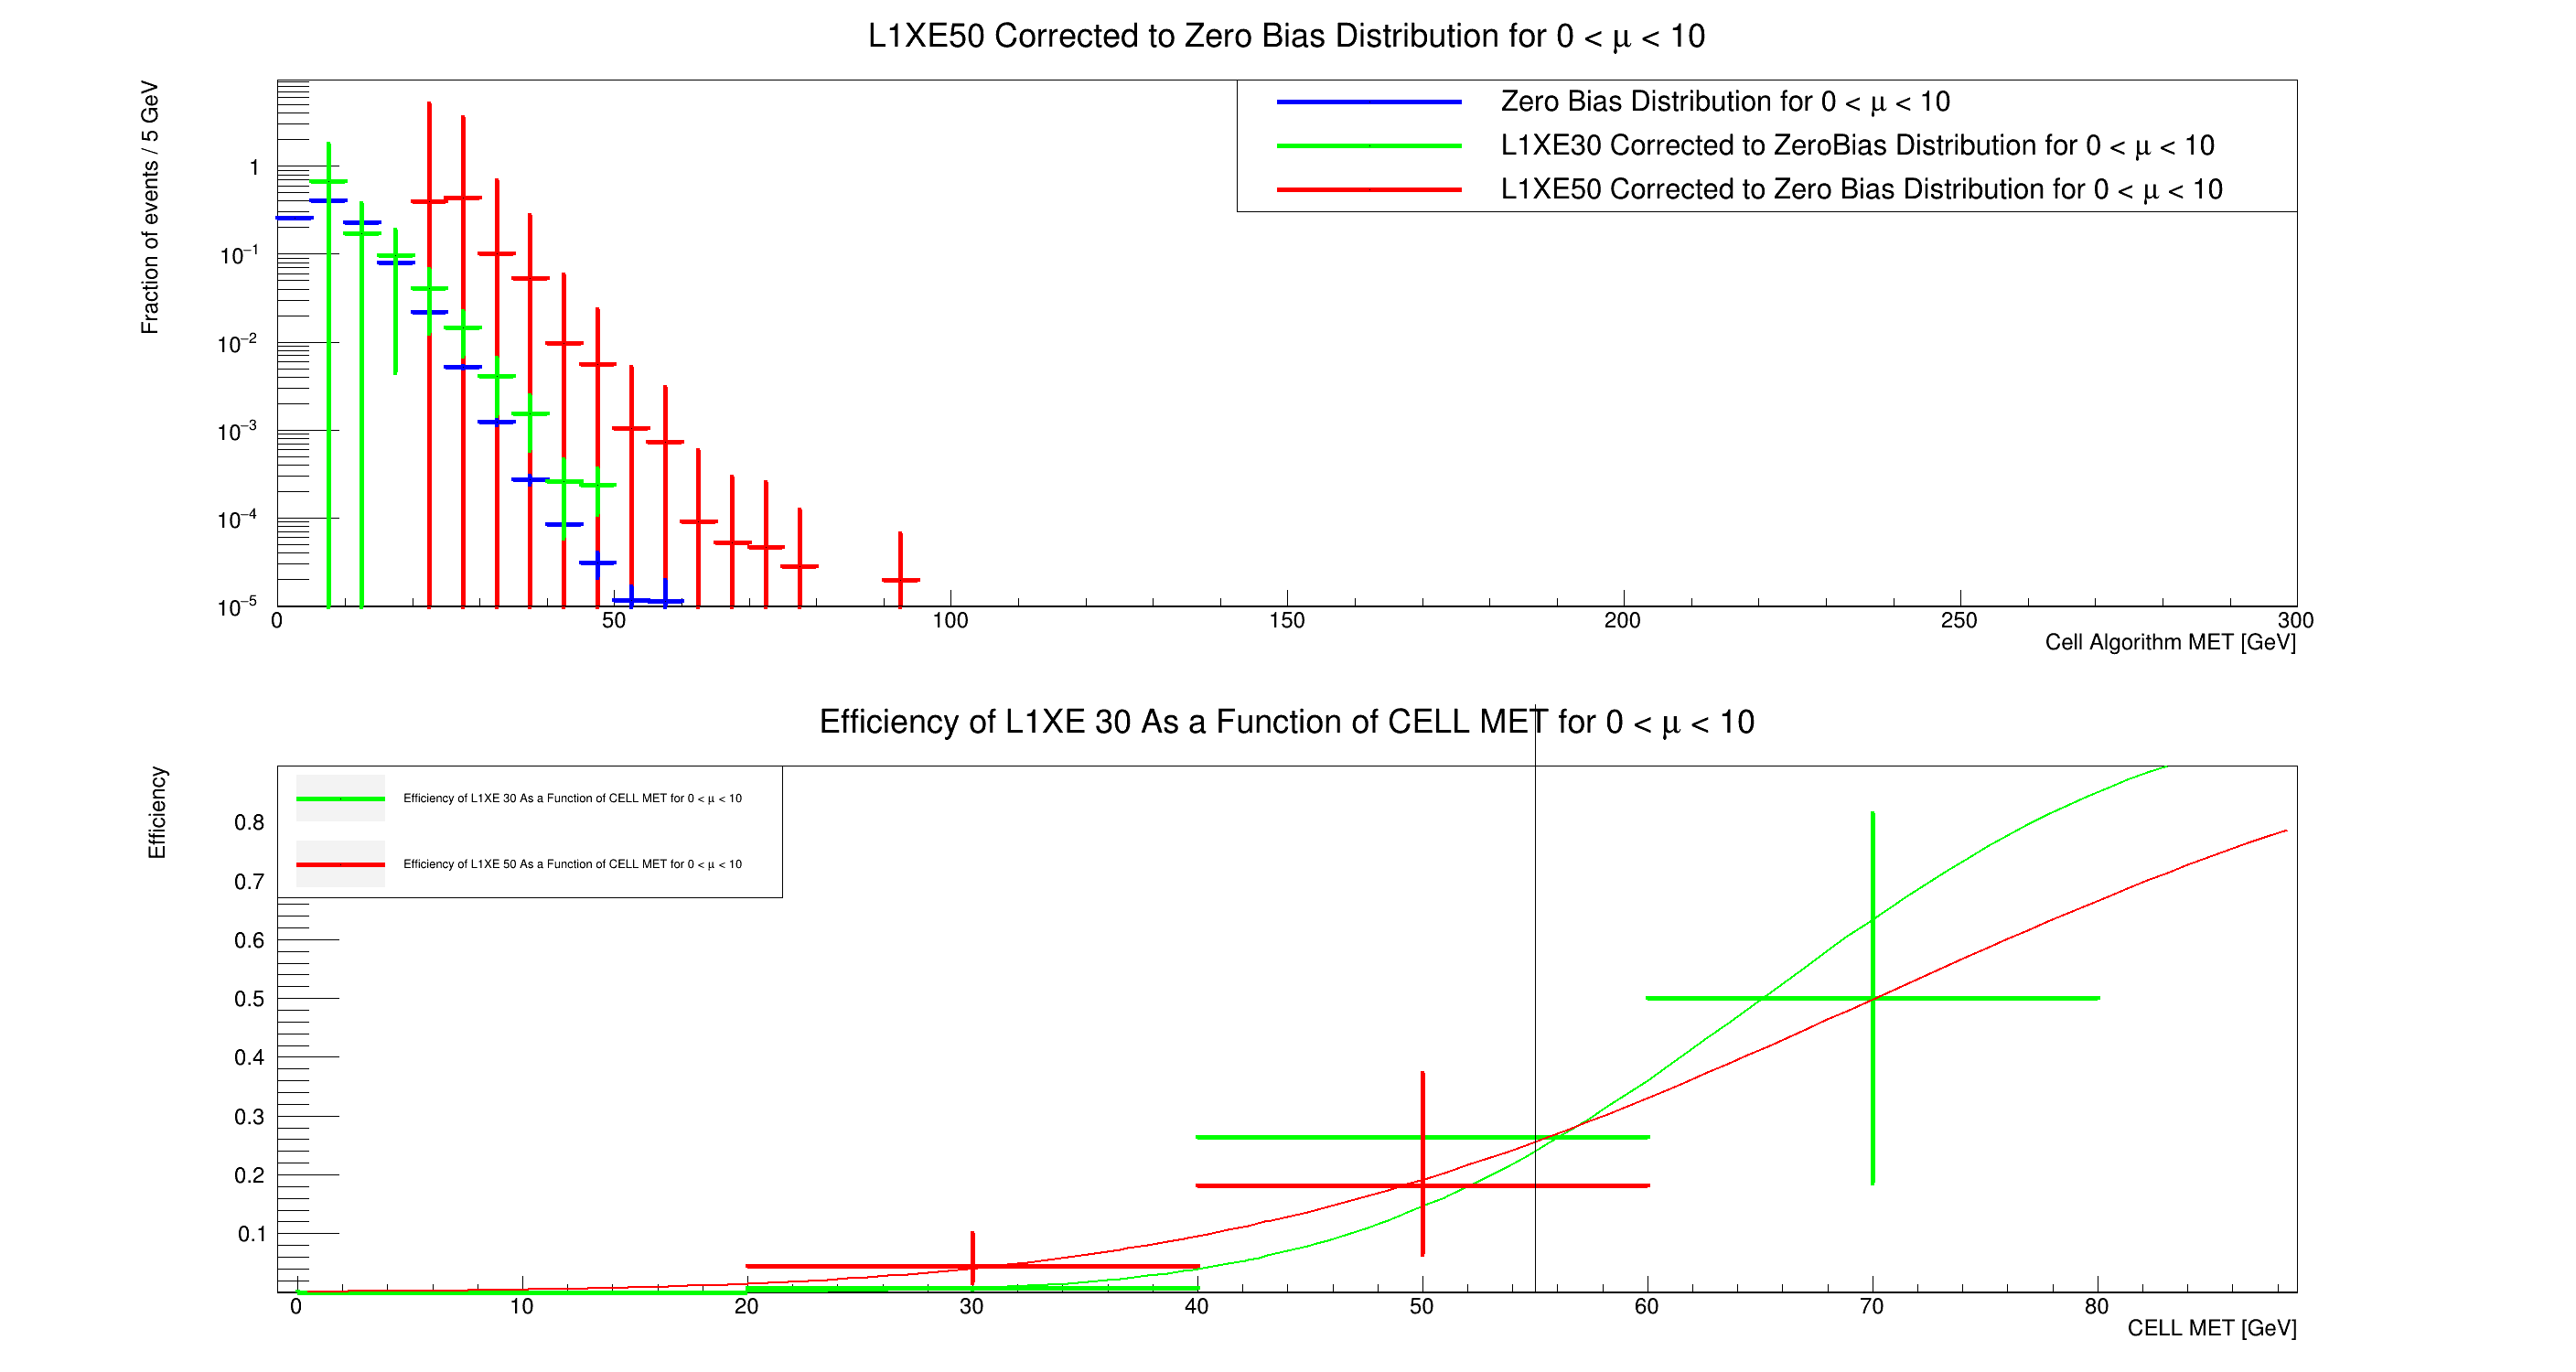
\includegraphics[height=2.65in,width=4.25in]{zerobias_distributions_corrected/zb_met_distributions_mubin_0}}
\end{frame}
\begin{frame}
        \frametitle{Unbiased Distributions for $10<\mu<20$}
        \framebox{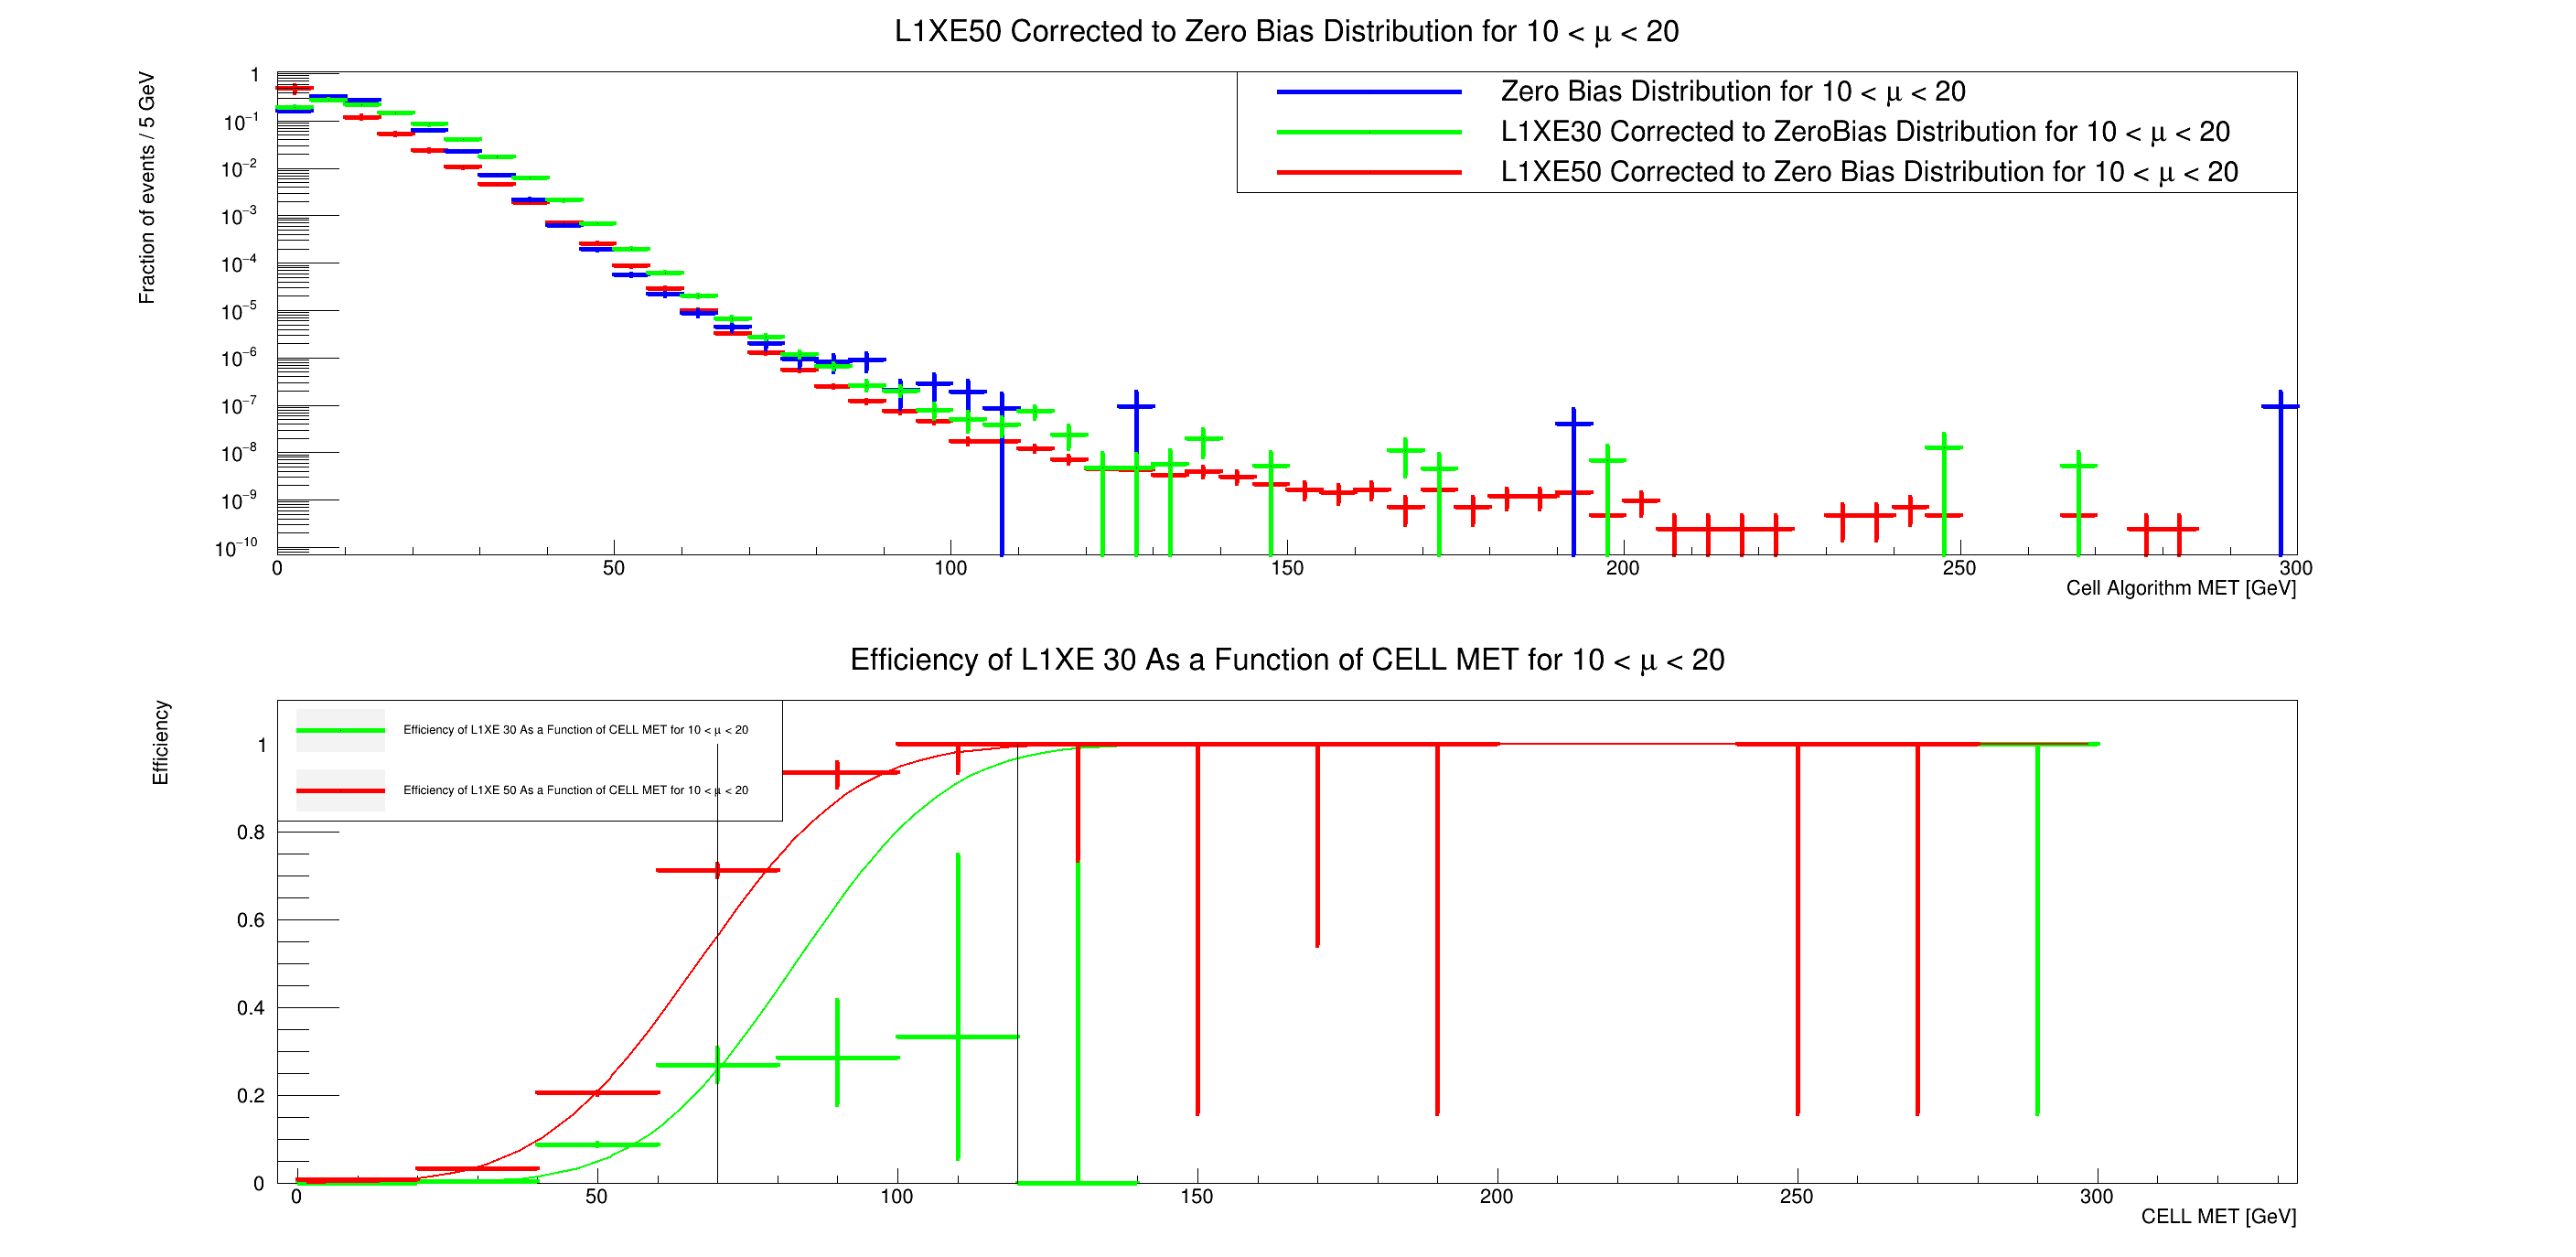
\includegraphics[height=2.65in,width=4.25in]{zerobias_distributions_corrected/zb_met_distributions_mubin_1}}
\end{frame}
\begin{frame}
        \frametitle{Unbiased Distributions for $20<\mu<30$}
        \framebox{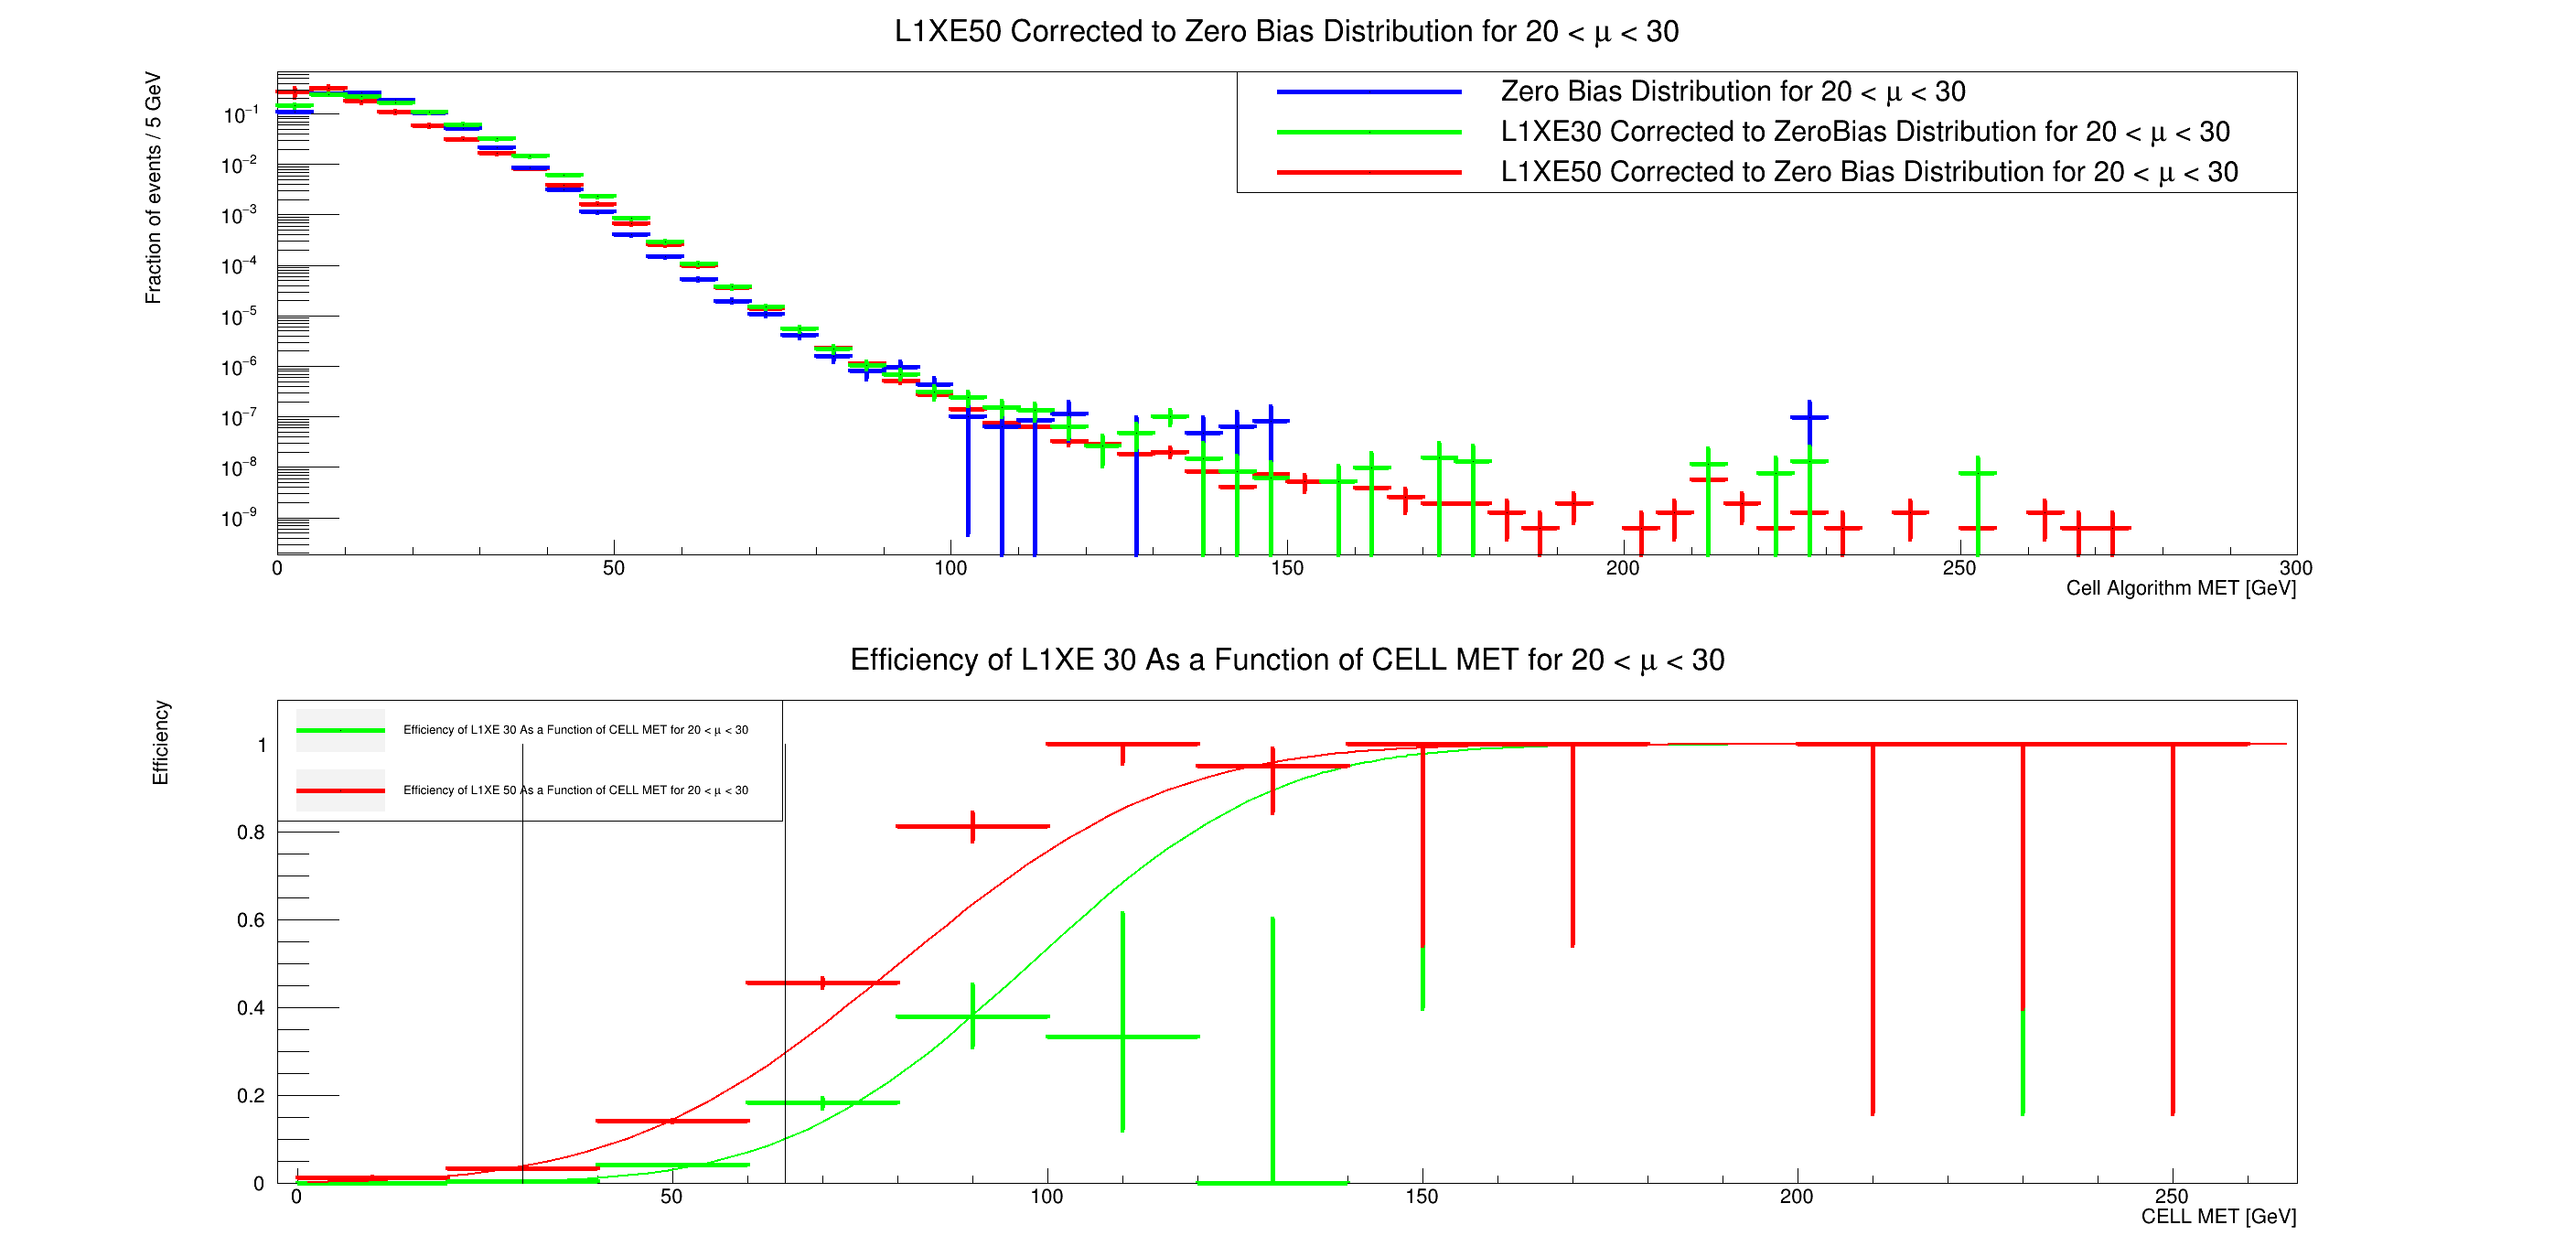
\includegraphics[height=2.65in,width=4.25in]{zerobias_distributions_corrected/zb_met_distributions_mubin_2}}
\end{frame}
\begin{frame}
        \frametitle{Unbiased Distributions for $30<\mu<40$}
        \framebox{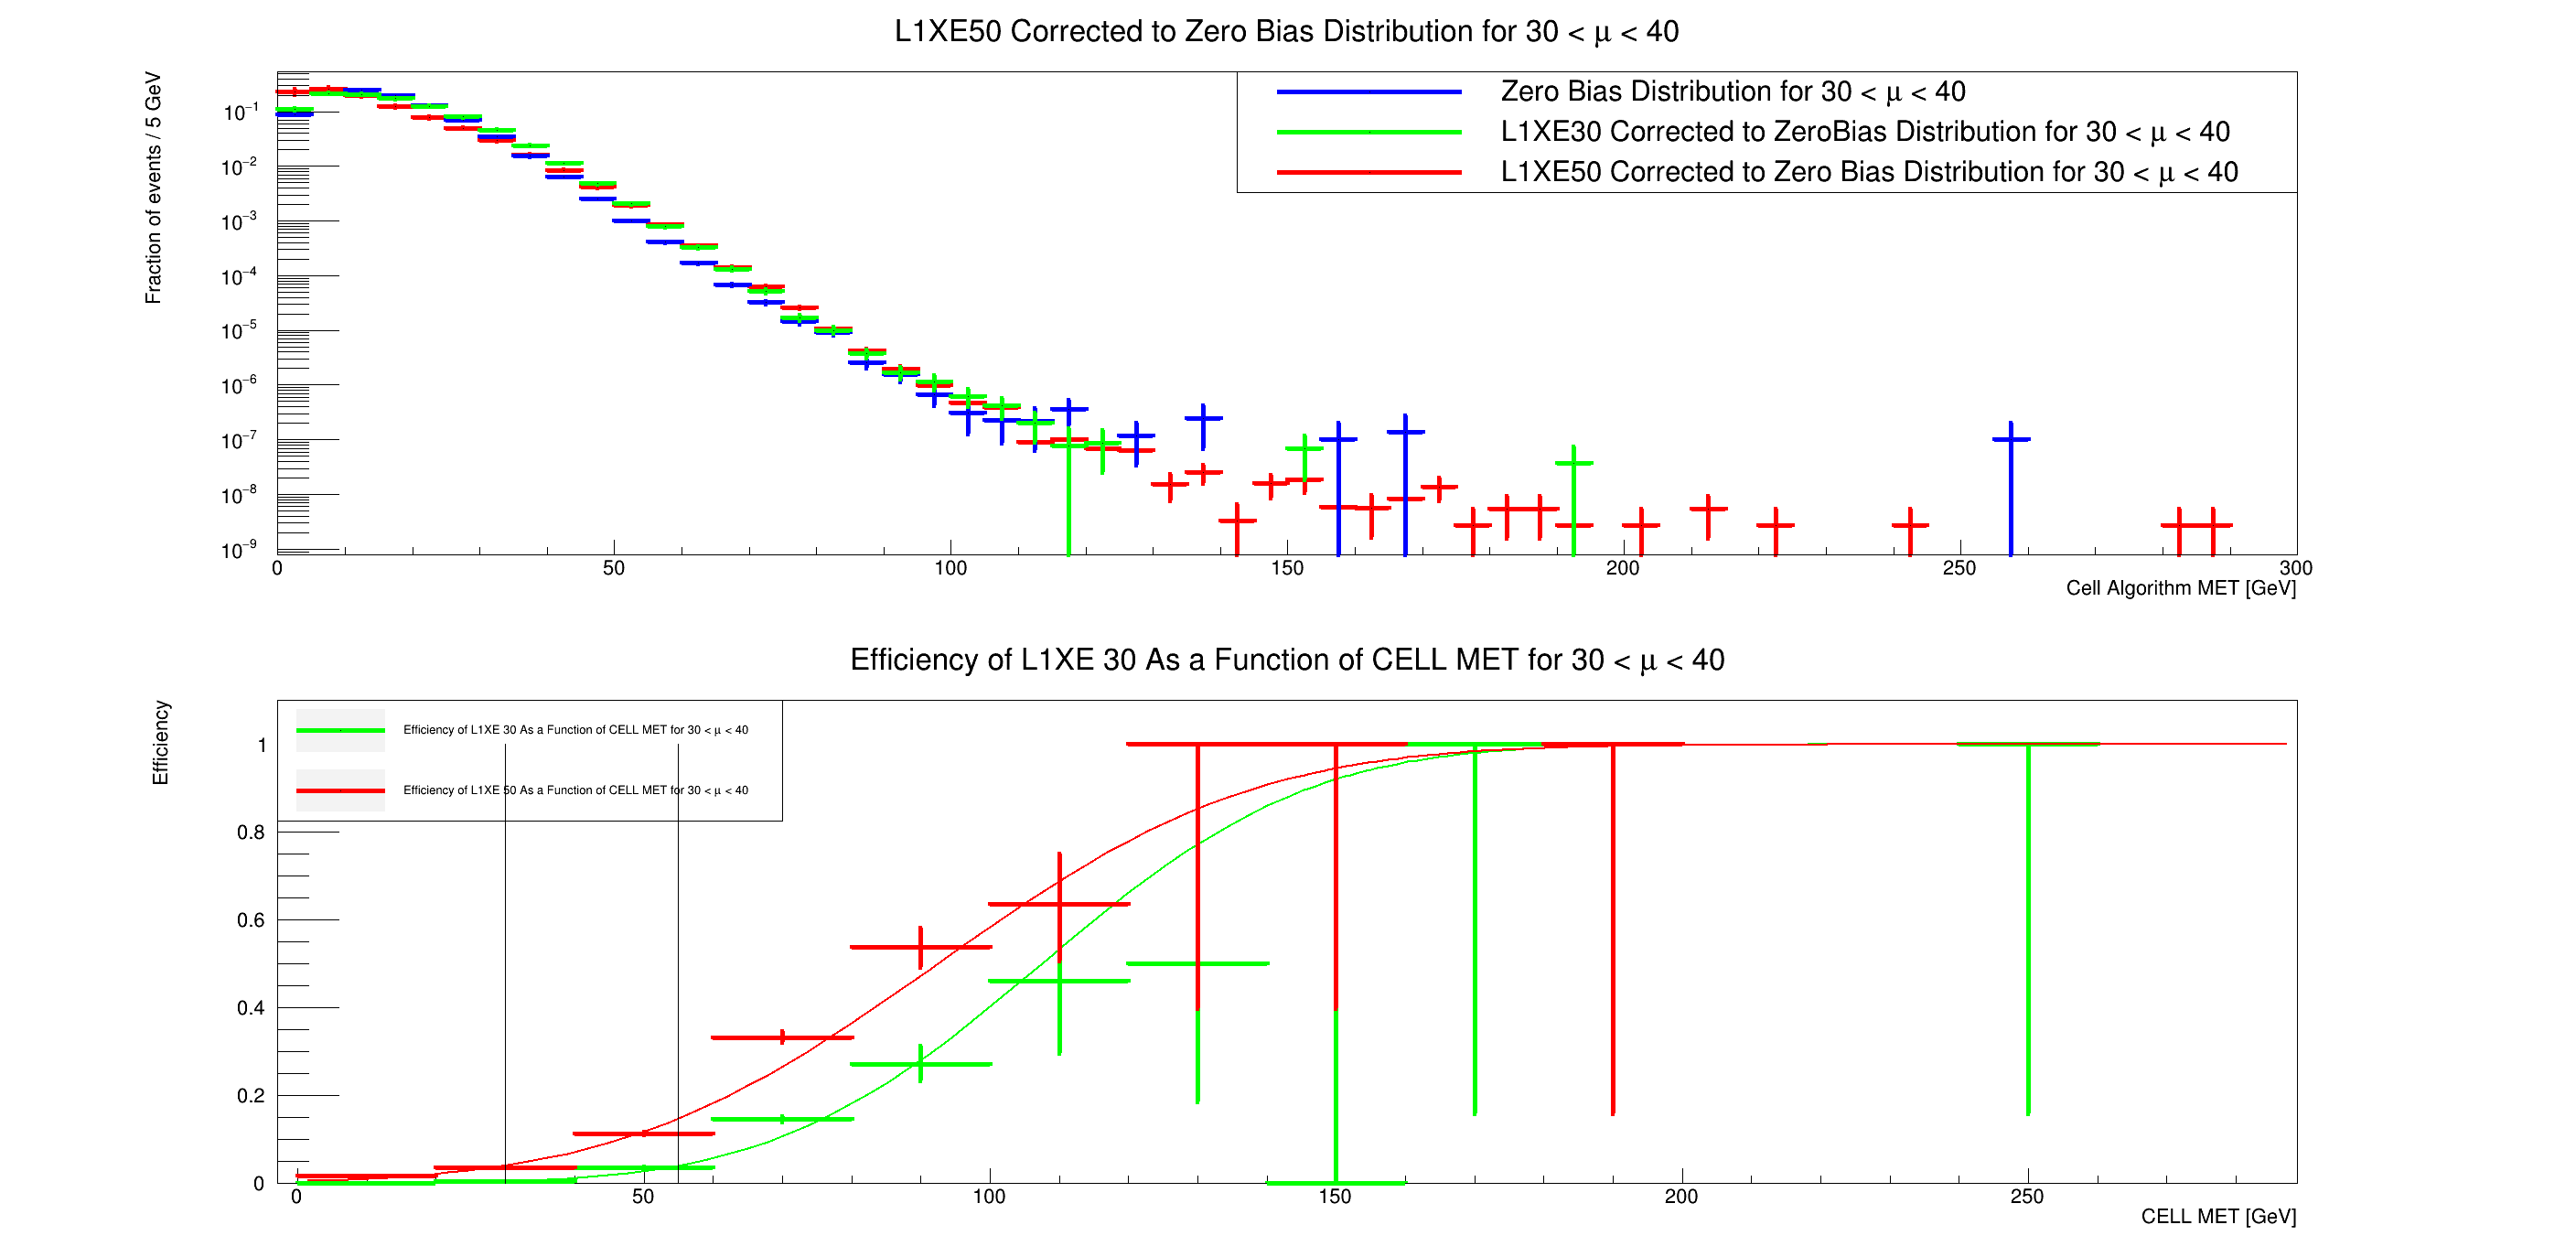
\includegraphics[height=2.65in,width=4.25in]{zerobias_distributions_corrected/zb_met_distributions_mubin_3}}
\end{frame}
\begin{frame}
        \frametitle{Unbiased Distributions for $40<\mu<50$}
        \framebox{\includegraphics[height=2.65in,width=4.25in]{zerobias_distributions_corrected/zb_met_distributions_mubin_4}}
\end{frame}
\begin{frame}
        \frametitle{Unbiased Distributions for $50<\mu<60$}
        \framebox{\includegraphics[height=2.65in,width=4.25in]{zerobias_distributions_corrected/zb_met_distributions_mubin_5}}
\end{frame}
\begin{frame}
        \frametitle{Unbiased Distributions for $60<\mu<70$}
        \framebox{\includegraphics[height=2.65in,width=4.25in]{zerobias_distributions_corrected/zb_met_distributions_mubin_6}}
\end{frame}
% RECONSTRUCTED DISTRIBUTIONS
\begin{frame}
        \frametitle{Reconstructed Unbiased CELL MET Distribution for $0<\mu<10$}
        \framebox{\includegraphics[height=2.65in,width=4.25in]{reconstructed_distributions/reconstructed_distribution_mubin_0}}
\end{frame}
\begin{frame}
        \frametitle{Reconstructed Unbiased CELL MET Distribution for $10<\mu<20$}
        \framebox{\includegraphics[height=2.65in,width=4.25in]{reconstructed_distributions/reconstructed_distribution_mubin_1}}
\end{frame}
\begin{frame}
        \frametitle{Reconstructed Unbiased CELL MET Distribution for $20<\mu<30$}
        \framebox{\includegraphics[height=2.65in,width=4.25in]{reconstructed_distributions/reconstructed_distribution_mubin_2}}
\end{frame}
\begin{frame}
        \frametitle{Reconstructed Unbiased CELL MET Distribution for $30<\mu<40$}
        \framebox{\includegraphics[height=2.65in,width=4.25in]{reconstructed_distributions/reconstructed_distribution_mubin_3}}
\end{frame}
\begin{frame}
        \frametitle{Reconstructed Unbiased CELL MET Distribution for $40<\mu<50$}
        \framebox{\includegraphics[height=2.65in,width=4.25in]{reconstructed_distributions/reconstructed_distribution_mubin_4}}
\end{frame}
\begin{frame}
        \frametitle{Reconstructed Unbiased CELL MET Distribution for $50<\mu<60$}
        \framebox{\includegraphics[height=2.65in,width=4.25in]{reconstructed_distributions/reconstructed_distribution_mubin_5}}
\end{frame}
\begin{frame}
        \frametitle{Reconstructed Unbiased CELL MET Distribution for $60<\mu<70$}
        \framebox{\includegraphics[height=2.65in,width=4.25in]{reconstructed_distributions/reconstructed_distribution_mubin_6}}
\end{frame}
% TABLE OF FIT PARAMETERS
\begin{frame}
\begin{table}[ht]
\caption{Fit Parameter Table}
\centering
\begin{tabular}{|c|c|c|c|c|}
\hline\hline
a & b & $\sigma$ & L1XE & $\mu$ bin\\ 
\hline
0.536043 & -4.88401 & 7.63437 & 30 & 0\\ 
0.449818 & 18.4754 & 10.3507 & 50 & 0\\ 
0.40883 & -3.87341 & 8.13195 & 30 & 1\\ 
0.505088 & 16.3944 & 10.3677 & 50 & 1\\ 
0.336915 & -2.90115 & 8.63962 & 30 & 2\\ 
0.345437 & 22.3296 & 9.83129 & 50 & 2\\ 
0.29943 & -2.17211 & 9.01473 & 30 & 3\\ 
0.277972 & 24.32 & 9.94887 & 50 & 3\\ 
0.281092 & -1.63701 & 9.27598 & 30 & 4\\ 
0.289215 & 22.6488 & 10.6932 & 50 & 4\\ 
0.2487 & -0.58147 & 9.68806 & 30 & 5\\ 
0.230607 & 24.8226 & 9.95501 & 50 & 5\\ 
0.231716 & 0.541431 & 9.99171 & 30 & 6\\ 
0.183126 & 26.0774 & 10.0148 & 50 & 6\\ 
\hline
\end{tabular}
\end{table}

\end{frame}
\end{document}
